% *************************************
% ------- PhD Thesis Anna Cuomo -------
% *************************************

\documentclass[a4paper,12pt,times,numbered,print]{Classes/PhDThesisPSnPDF}

% *************************************
% **** Class Options 
% *************************************

% `a4paper'(The University of Cambridge PhD thesis guidelines recommends a page size a4 - default option) or `a5paper': A5 Paper size is also allowed as per the Cambridge University Engineering Deparment guidelines for PhD thesis

% `11pt' or `12pt'(default): Font Size 10pt is NOT recommended by the University guidelines

% `oneside' or `twoside'(default): Printing double side (twoside) or single side.

% `print': Use `print' for print version with appropriate margins and page layout. Leaving the options field blank will activate Online version.

% `index': For index at the end of the thesis

% `draftclassic': For draft mode without loading any images (same as draft in book)

% `draft': Special draft mode with line numbers, images, and water mark with timestamp and custom text. Position of the text can also be modified.

% `abstract': To generate only the title page and abstract page with
% dissertation title and name, to submit to the Student Registry

% `chapter`: This option enables only the specified chapter and it's references. Useful for review and corrections.

% *************************************
% **** Custom Page Margins 
% *************************************

% `custommargin`: Use `custommargin' in options to activate custom page margins, which can be defined in the preamble.tex. Custom margin will override print/online margin setup.

% *************************************
% **** Choosing the Fonts in Class Options 
% *************************************

% `times' : Times font with math support. (The Cambridge University guidelines recommend using times)

% `fourier': Utopia Font with Fourier Math font (Font has to be installed)      

% `customfont': Use `customfont' option in the document class and load the package in the preamble.tex

% default or leave empty: `Latin Modern' font will be loaded.

% *************************************
% **** Choosing the Bibliography style 
% *************************************

% `authoryear': For author-year citation eg., Krishna (2013)

% `numbered': (Default Option) For numbered and sorted citation e.g., [1,5,2]

% `custombib': Define your own bibliography style in the `preamble.tex' file. `\RequirePackage[square, sort, numbers, authoryear]{natbib}'.cThis can be also used to load biblatex instead of natbib (See Preamble)

% *************************************
% **** Choosing the Page Style 
% *************************************

% `default (leave empty)': For Page Numbers in Header (Left Even, Right Odd) and Chapter Name in Header (Right Even) and Section Name (Left Odd). Blank Footer.

% `PageStyleI': Chapter Name next & Page Number on Even Side (Left Even).  Section Name & Page Number in Header on Odd Side (Right Odd). Footer is empty.

% `PageStyleII': Chapter Name on Even Side (Left Even) in Header. Section Number and Section Name in Header on Odd Side (Right Odd). Page numbering in footer

% Uncomment to change page style
%\pagestyle{PageStyleII}

% *************************************
% **** Preamble 
% *************************************

% ******************************************************************************
% ****************************** Custom Margin *********************************

% Add `custommargin' in the document class options to use this section
% Set {innerside margin / outerside margin / topmargin / bottom margin}  and
% other page dimensions
\ifsetCustomMargin
  \RequirePackage[left=37mm,right=30mm,top=35mm,bottom=30mm]{geometry}
  \setFancyHdr % To apply fancy header after geometry package is loaded
\fi

% Add spaces between paragraphs
%\setlength{\parskip}{0.5em}
% Ragged bottom avoids extra whitespaces between paragraphs
\raggedbottom
% To remove the excess top spacing for enumeration, list and description
%\usepackage{enumitem}
%\setlist[enumerate,itemize,description]{topsep=0em}

% No indent before paragraph
\setlength\parindent{0pt}

% *****************************************************************************
% ******************* Fonts (like different typewriter fonts etc.)*************

% Add `customfont' in the document class option to use this section

\ifsetCustomFont
  % Set your custom font here and use `customfont' in options. Leave empty to
  % load computer modern font (default LaTeX font).
  %\RequirePackage{helvet}

  % For use with XeLaTeX
  %  \setmainfont[
  %    Path              = ./libertine/opentype/,
  %    Extension         = .otf,
  %    UprightFont = LinLibertine_R,
  %    BoldFont = LinLibertine_RZ, % Linux Libertine O Regular Semibold
  %    ItalicFont = LinLibertine_RI,
  %    BoldItalicFont = LinLibertine_RZI, % Linux Libertine O Regular Semibold Italic
  %  ]
  %  {libertine}
  %  % load font from system font
  %  \newfontfamily\libertinesystemfont{Linux Libertine O}
  
  % Use helvetica
  \renewcommand{\familydefault}{\sfdefault}
  \usepackage{helvet}
  \usepackage{sansmathfonts}
\fi

% *********
% ***** Custom Packages

% define header 
\usepackage{fancyhdr}
\usepackage{adjustbox}
\usepackage{etoolbox}
\renewcommand{\headrulewidth}{1pt}
\newcommand{\headrulecolor}[1]{\patchcmd{\headrule}{\hrule}{\color{#1}\hrule}{}{}}
\headrulecolor{CadetBlue}
\fancyheadoffset[RE,LO]{0cm}
\fancyheadoffset[LE,RO]{1.25cm}

% For recoloring the section header
\usepackage{sectsty}
\definecolor{dark-gray}{gray}{0.30}
\sectionfont{\color{dark-gray}}
\subsectionfont{\color{dark-gray}}
% \subsubsectionfont{\color{dark-gray}}

% Fancier section header
\newcommand{\hsp}{\hspace{6pt}}
\usepackage[explicit]{titlesec}
\titleformat{\section}[hang]{\Large\bfseries}{\color{dark-gray}\thesection}{6pt}{\begin{tabular}[t]{@{\color{dark-gray}\vrule width 2pt}>{\hsp}l}#1\end{tabular}}
\titleformat{\subsection}[hang]{\large\bfseries}{\color{dark-gray}\thesubsection}{6pt}{\begin{tabular}[t]{@{\color{dark-gray}\vrule width 2pt}>{\hsp}l}#1\end{tabular}}



% **** Algorithms and Pseudocode 

%\usepackage{algpseudocode}


% **** Captions and Hyperreferencing / URL 

% Captions: This makes captions of figures use a boldfaced small font.
\usepackage[font=small,labelfont=bf]{caption}
\DeclareCaptionLabelFormat{adja-page}{\hrulefill\\#1 #2 \emph{(previous page)}}

%\RequirePackage[labelsep=space,tableposition=top]{caption}
\renewcommand{\figurename}{Fig.} %to support older versions of captions.sty

\usepackage{hyperref}
\hypersetup{
    colorlinks=true,
    linkcolor=black,
    filecolor=black,      
    urlcolor=blue,
}


% *************************** Graphics and figures *****************************

%\usepackage{rotating}
\usepackage{wrapfig}

% Uncomment the following two lines to force Latex to place the figure.
% Use [H] when including graphics. Note 'H' instead of 'h'
%\usepackage{float}
%\restylefloat{figure}

% Subcaption package is also available in the sty folder you can use that by
% uncommenting the following line
% This is for people stuck with older versions of texlive
%\usepackage{sty/caption/subcaption}
\usepackage{subcaption}

% ********************************** Tables ************************************
\usepackage{booktabs} % For professional looking tables
\usepackage{multirow}

%\usepackage{multicol}
%\usepackage{longtable}
%\usepackage{tabularx}


% *********************************** SI Units *********************************
\usepackage{siunitx} % use this package module for SI units
\usepackage{textcomp} % for trademark


% ******************************* Line Spacing *********************************

% Choose linespacing as appropriate. Default is one-half line spacing as per the
% University guidelines

% \doublespacing
% \onehalfspacing
% \singlespacing


% ************************ Formatting / Footnote *******************************

% Don't break enumeration (etc.) across pages in an ugly manner (default 10000)
%\clubpenalty=500
%\widowpenalty=500

%\usepackage[perpage]{footmisc} %Range of footnote options

% Nicer heading
\renewcommand{\chaptername}{}
\usepackage[Lenny]{fncychap}


% *****************************************************************************
% *************************** Bibliography  and References ********************

%\usepackage{cleveref} %Referencing without need to explicitly state fig /table

% Add `custombib' in the document class option to use this section
\ifuseCustomBib
   \RequirePackage[square, sort, numbers, authoryear]{natbib} % CustomBib

% If you would like to use biblatex for your reference management, as opposed to the default `natbibpackage` pass the option `custombib` in the document class. Comment out the previous line to make sure you don't load the natbib package. Uncomment the following lines and specify the location of references.bib file

%\RequirePackage[backend=biber, style=numeric-comp, citestyle=numeric, sorting=nty, natbib=true]{biblatex}
%\addbibresource{References/references} %Location of references.bib only for biblatex, Do not omit the .bib extension from the filename.

\fi

% changes the default name `Bibliography` -> `References'
\renewcommand{\bibname}{References}


% ******************************************************************************
% ************************* User Defined Commands ******************************
% ******************************************************************************

% **** To change the name of Table of Contents / LOF and LOT 
\usepackage{tocloft}
\setlength\cftaftertoctitleskip{0pt}
\setlength\cftafterloftitleskip{0pt}
\setlength\cftafterlottitleskip{0pt}
\renewcommand\cfttoctitlefont{\LARGE\bfseries\scshape\color{CadetBlue}}
\renewcommand\cftloftitlefont{\LARGE\bfseries\scshape\color{CadetBlue}}
\renewcommand\cftlottitlefont{\LARGE\bfseries\scshape\color{CadetBlue}}

%\renewcommand{\glossarysection}[2][\theglstoctitle]{%
%  \def\theglstoctitle{#2}%
%  \vspace{\cftbeforelottitleskip}%
%  \par\noindent
%  \addcontentsline{toc}{chapter}{\numberline{}#1}%
%}

%\renewcommand{\contentsname}{\textcolor{Mahogany}{\LARGE \textbf{\textsc{Table of contents}}}}
%\renewcommand{\listfigurename}{\textcolor{Mahogany}{\LARGE \textbf{\textsc{List of figures}}}}
%\renewcommand{\listtablename}{\textcolor{Mahogany}{\LARGE \textbf{\textsc{List of tables}}}}

% Math abbreviations
\newcommand{\iid}{\stackrel{\mbox{iid}}{\sim}}
\newcommand{\ind}{\stackrel{\mbox{ind}}{\sim}}
\newcommand{\Lagr}{\mathcal{L}}
\newcommand{\plus}{\textsuperscript{+}}
\usepackage{tikz}
\def\checkmark{\tikz\fill[scale=0.4](0,.35) -- (.25,0) -- (1,.7) -- (.25,.15) -- cycle;} 



% ********************** TOC depth and numbering depth *************************

\setcounter{secnumdepth}{2}
\setcounter{tocdepth}{2}


% ******************************* Nomenclature 
%\usepackage{nomencl}
%\renewcommand{\nomname}{Symbols}
%\makenomenclature

\usepackage[acronym, nopostdot, nonumberlist, style=super]{glossaries}
\setlength{\glsdescwidth}{5in}

\makeglossaries
\glsdisablehyper
\renewcommand{\glsnamefont}[1]{\textbf{#1}}

% ********************************* Appendix 

% The default value of both \appendixtocname and \appendixpagename is `Appendices'. These names can all be changed via:

%\renewcommand{\appendixtocname}{List of appendices}
%\renewcommand{\appendixname}{Appndx}

% *********************** Configure Draft Mode **********************************

% Uncomment to disable figures in `draft'
%\setkeys{Gin}{draft=true}  % set draft to false to enable figures in `draft'

% These options are active only during the draft mode
% Default text is "Draft"
%\SetDraftText{DRAFT}

% Default Watermark location is top. Location (top/bottom)
%\SetDraftWMPosition{bottom}

% Draft Version - default is v1.0
%\SetDraftVersion{v1.1}

% Draft Text grayscale value (should be between 0-black and 1-white)
% Default value is 0.75
%\SetDraftGrayScale{0.8}


% ******************************** Todo Notes **********************************

% Define colour for todo notes
\newcommand{\todo}[1]{{\color{red}{#1}}}
% Colour for corrections
\newcommand{\cor}[1]{{\color{blue}{#1}}}

% *****************************************************************************
% ******************* Better enumeration my MB*************
\usepackage{enumitem}

% **********************************
% Additional packages
\usepackage{xcolor}
\definecolor{green}{RGB}{32,157,148}
\usepackage{amsmath,amsfonts,amssymb,amsthm,nccmath,systeme} % For math equations, theorems, symbols, etc
\DeclareMathAlphabet{\mathcal}{OMS}{cmsy}{m}{n} % reset mathcal to normal
\usepackage{bm} % bold math 
\usepackage{textgreek} % greek letters in text

%----------------------------------------------------------------------------------------
%	THEOREM STYLES
%----------------------------------------------------------------------------------------

%%%%%%%%%%%%%%%%%%%%%%%%%%%%%%%%%%%%%%%%%%%%%%%%%%%%%%%%%
%%% dedicated to boxed/framed environements %%%%%%%%%%%%%
%%%%%%%%%%%%%%%%%%%%%%%%%%%%%%%%%%%%%%%%%%%%%%%%%%%%%%%%%

\newtheoremstyle{greennumbox}% % Theorem style name
{0pt}% Space above
{0pt}% Space below
{\small}% % Body font
{}% Indent amount
{\small\bf\sffamily\color{green}}% % Theorem head font
{\;}% Punctuation after theorem head
{0.25em}% Space after theorem head
{\small\sffamily\color{green}\thmname{}\nobreakspace} 
\renewcommand{\qedsymbol}{$\blacksquare$}% Optional qed square

\newtheoremstyle{blacknumbox} % Theorem style name
{0pt}% Space above
{0pt}% Space below
{\normalfont}% Body font
{}% Indent amount
{\small\bf\sffamily}% Theorem head font
{}% Punctuation after theorem head
{0.25em}% Space after theorem head
{\small\sffamily\thmname{}\nobreakspace}

\newtheoremstyle{bluenumbox} % Theorem style name
{0pt}% Space above
{0pt}% Space below
{\normalfont}% Body font
{}% Indent amount
{\small\bf\sffamily\color{blue}}% Theorem head font
{}% Punctuation after theorem head
{0.25em}% Space after theorem head
{\small\sffamily\thmname{}\nobreakspace}

% Defines the theorem text style for each type of theorem to one of the three styles above
\theoremstyle{greennumbox}
\newtheorem{abstractT}{}
\theoremstyle{bluenumbox}
\newtheorem{boxT}{}
\theoremstyle{blacknumbox}
\newtheorem{commentT}{}


% Package to create coloured boxes
\RequirePackage[framemethod=default]{mdframed}

% Exercise box	  
\newmdenv[skipabove=7pt,
skipbelow=7pt,
rightline=false,
leftline=true,
topline=false,
bottomline=false,
backgroundcolor=green!10,
linecolor=green,
innerleftmargin=5pt,
innerrightmargin=5pt,
innertopmargin=5pt,
innerbottommargin=5pt,
leftmargin=0cm,
rightmargin=0cm,
linewidth=4pt]{eBox}

\definecolor{cornflowerblue}{RGB}{114,133,165}

\newmdenv[skipabove=10pt,
skipbelow=7pt,
rightline=false,
leftline=true,
topline=false,
bottomline=false,
backgroundcolor=cornflowerblue!10,
linecolor=cornflowerblue,
innerleftmargin=5pt,
innerrightmargin=5pt,
innertopmargin=5pt,
innerbottommargin=5pt,
leftmargin=0cm,
rightmargin=0cm,
linewidth=4pt
innerbottommargin=5pt]{bBox}

\newmdenv[skipabove=7pt,
skipbelow=7pt,
rightline=false,
leftline=true,
topline=false,
bottomline=false,
linecolor=gray,
backgroundcolor=black!5,
innerleftmargin=5pt,
innerrightmargin=5pt,
innertopmargin=5pt,
leftmargin=0cm,
rightmargin=0cm,
linewidth=4pt,
innerbottommargin=5pt]{cBox}

% Creates an environment for each type of theorem and assigns it a theorem text style from the "Theorem Styles" section above and a colored box from above

% \newenvironment{Abstract}{\begin{eBox}\begin{abstractT}}{\hfill{\color{green}\tiny\ensuremath{\blacksquare}}\end{abstractT}\end{eBox}}
\newenvironment{Abstract}{\begin{eBox}\begin{abstractT}}{\end{abstractT}\end{eBox}}
\newenvironment{Comment}{\begin{cBox}\begin{commentT}}{\end{commentT}\end{cBox}}	\newenvironment{Comment2}{\begin{bBox}\begin{boxT}}{\end{boxT}\end{bBox}}


%!TEX root = ../thesis.tex
%******************************
%	 Acronyms 
%*****************************

\newacronym{ase}{ASE}{allele-specific expression}
\newacronym{bh}{BH}{Benjamini-Hochberg}
\newacronym{blup}{BLUP}{Best linear unbiased predictor}
\newacronym{bmi}{BMI}{body mass index}
\newacronym{bp}{bp}{base pair}
\newacronym{chipseq}{ChIP-seq}{Chromatin immuno-precipitation sequencing}
\newacronym{CD/CV}{CD/CV}{Common disease / common variant}
\newacronym{cpm}{CPM}{counts per million (reads)}
\newacronym{cv}{CV}{coefficient of variation}
\newacronym{da}{DA}{dopaminergic neurons}
\newacronym{defendo}{defendo}{definitive endoderm}
\newacronym{dna}{DNA}{deoxyribonucleic acid} 
\newacronym{dof}{dof}{degrees of freedom}
\newacronym{ebi}{EBI}{European Bioinformatics Institute}
\newacronym[plural=eQTL, firstplural=expression quantitative trait loci (eQTL)]{eqtl}{eQTL}{expression quantitative trait locus}
\newacronym{es}{ES}{embryonic stem}
\newacronym[plural=ESCs, firstplural=embryonic stem cells (ESCs)]{esc}{ESC}{embryonic stem cell}
\newacronym{facs}{FACS}{fluorescence-activated cell sorting}
\newacronym{fdr}{FDR}{false discovery rate}
\newacronym{gxe}{GxE}{genotype-environment}
\newacronym{glm}{GLM}{generalised linear model}
\newacronym{gtex}{GTEx}{genotype-tissue expression}
\newacronym[plural=GWAS, firstplural=genome-wide association studies (GWAS)]{gwas}{GWAS}{genome-wide association study}
\newacronym[plural=hESCs, firstplural=human embryonic stem cells (hESCs)]{hesc}{hESC}{human embryonic stem cell}
\newacronym{hgp}{HGP}{Human Genome Project}
\newacronym{hipsci}{HipSci}{human induced pluripotent stem cell initiative}
\newacronym{hvgs}{HVGs}{highly variable genes}
\newacronym{ips}{iPS}{induced pluripotent stem}
\newacronym[plural=iPSCs, firstplural=induced pluripotent stem cells (iPSCs)]{ipsc}{iPSC}{induced pluripotent stem cell}
\newacronym{ivf}{IVF}{\textit{in vitro} fertilisation}
\newacronym{kb}{kb}{kilobase (pair)}
\newacronym{ld}{LD}{linkage disequilibrium}
\newacronym[plural=LMMs, firstplural=linear mixed models (LMMs)]{lmm}{LMM}{linear mixed model}
\newacronym{lrt}{LRT}{likelihood ratio test}
\newacronym{maf}{MAF}{minor allele frequency}
\newacronym{mesendo}{mesendo}{mesendoderm}
\newacronym{ml}{ML}{maximum likelihood}
\newacronym{mle}{MLE}{maximum likelihood estimator}
\newacronym{mqtl}{mQTL}{(DNA) methylation QTL}
\newacronym{mrna}{mRNA}{messenger RNA}
\newacronym{ngs}{NGS}{next generation sequencing}
\newacronym{nhgri}{NHGRI}{National Human Genome Research Institute}
\newacronym{ols}{OLS}{ordinary least squares}
\newacronym{pbmc}{PBMC}{peripheral blood mononuclear cell}
\newacronym[plural=PCs, firstplural=principal components (PCs)]{pc}{PC}{principal component}
\newacronym{pca}{PCA}{principal component analysis}
\newacronym{qc}{QC}{quality control}
\newacronym{qq}{QQ}{quantile-quantile}
\newacronym{qtl}{QTL}{quantitative trait locus}
\newacronym{qtls}{QTL}{quantitative trait loci}
\newacronym{scrnaseq}{scRNA-seq}{single-cell RNA sequencing} 
\newacronym{rna}{RNA}{ribonucleic acid}
\newacronym{rnaseq}{RNA-seq}{RNA sequencing}
\newacronym{scnt}{SCNT}{somatic-cell nuclear transfer}
\newacronym[plural=SNPs, firstplural=single nucleotide polymorphisms (SNPs)]{snp}{SNP}{single nucleotide polymorphism}
\newacronym{tf}{TF}{transcription factor}
\newacronym{trna}{tRNA}{transfer RNA}
\newacronym{tss}{TSS}{transcription start site}
\newacronym[plural=UMIs, firstplural=unique molecular identifiers (UMIs)]{umi}{UMI}{unique molecular identifier}

% *************************************
% **** Thesis Information & Meta-data 
% *************************************

% ************************ Thesis Information & Meta-data **********************
%% The title of the thesis
\title{Using single-cell RNA-seq to assess the effect of common genetic variants on gene expression during development}
% \title{Uncovering genetic effects on gene expression in differentiating iPS cells at single cell resolution}
%\texorpdfstring is used for PDF metadata. Usage:
%\texorpdfstring{LaTeX_Version}{PDF Version (non-latex)} eg.,
%\texorpdfstring{$sigma$}{sigma}


%% The full name of the author
\author{Anna Cuomo}

%% Department (eg. Department of Engineering, Maths, Physics)
\dept{European Bioinformatics Institute}

%% University and Crest
\university{University of Cambridge}
% Crest minimum should be 30mm.
\crest{
\includegraphics[width=0.2\textwidth]{University_Crest}}
%% Use this crest, if you are using the college crest
%% Crest long miminum should be 65mm
%\crest{
\includegraphics[width=0.45\textwidth]{University_Crest_Long}}

%% College shield [optional] 
% Crest minimum should be 30mm.
%\collegeshield{
\includegraphics[width=0.2\textwidth]{CollegeShields/Kings}}


%% Supervisor (optional)
%% for multiple supervisors, append each supervisor with the \newline command
%\supervisor{Prof. A.B. Supervisor\newline
%Prof. C.D. Supervisor}

%% Supervisor Role (optional) - Supervisor (default) or advisor
% \supervisorrole{\textbf{Supervisors: }}
%% if no title is desired:
% \supervisorrole{}

%% Supervisor line width: required to align supervisors
%\supervisorlinewidth{0.35\textwidth}

%% Advisor (optional)
%% for multiple advisors, append each advisor with the \newline command
%\advisor{Dr. A. Advisor\newline
%Dr. B. Advisor}
     
%% Advisor Role (optional) - Advisor (default) or leave empty
% \advisorrole{Advisors: }
%% if no title is required
% \advisorrole{}

%% Advisor line width: required to align supervisors
%\advisorlinewidth{0.25\textwidth}


%% You can redefine the submission text:
% Default as per the University guidelines:
% ``This dissertation is submitted for the degree of''
%\renewcommand{\submissiontext}{change the default text here if needed}

%% Full title of the Degree
\degreetitle{Doctor of Philosophy}

%% College affiliation (optional)
\college{Peterhouse College}

%% Submission date
% Default is set as {\monthname[\the\month]\space\the\year}
%\degreedate{September 2014} 

%% Meta information
\subject{LaTeX} \keywords{{LaTeX} {PhD Thesis} {EBI} {University of
Cambridge}}


% *************************************
% ***** Abstract 
% *************************************

\ifdefineAbstract
 \pagestyle{empty}
 \includeonly{Declaration/declaration, Abstract/abstract}
\fi

% *************************************
% **** Chapter Mode 
% *************************************
% The chapter mode allows user to only print particular chapters with references. Title, Contents, Frontmatter are disabled by default. Useful option to review a particular chapter or to send it to supervisior. To use choose `chapter' option in the document class

\ifdefineChapter
 \includeonly{Introduction/intro}
\fi

% *************************************
% **** Front Matter 
% *************************************

\begin{document}

\frontmatter

\maketitle

% ******************************* Thesis Dedication ********************************

\begin{dedication} 

\textit{“Nothing in life is to be feared, it is only to be understood.”}\\
\rightline{Marie Curie}

\end{dedication}
% ******************************* Thesis Declaration ***************************

\begin{declaration}

I hereby declare that except where specific reference is made to the work of  others, the contents of this dissertation are original and have not been  submitted in whole or in part for consideration for any other degree or qualification in this, or any other university. 
This dissertation is my own work and contains nothing which is the outcome of work done in collaboration with others, except as specified in the text and Contribution sections at the beginning of each chapter. 
This dissertation contains fewer than 60,000 words including appendices, bibliography, footnotes, tables and equations and has fewer than 150 figures.

% Author and date will be inserted automatically from thesis.tex \author \degreedate

\end{declaration}
% ************************** Thesis Acknowledgements **************************

\begin{acknowledgements}      


And I would like to acknowledge ...

John Marioni and Oliver Stegle

working together: Daniel Seaton, Marc Bonder, Julie Jerber, Danilo Horta, Davis McCarthy, Na Cai

reading and commenting thesis: 
Shila Ghazanfar, (ch2,ch3)
Nils Eling, (ch4)
Julie Jerber  (ch1.2)
% Rebecca Berrens (ch1.2)
Daniel Seaton (ch1)
% Marc Jan Bonder (ch2)
% Mike Morgan (ch2)
% Ximena Ibarra-Soria (ch4)
% Chris Laumer (ch1,ch5)
% Danila Bredikhin
% Paolo Casale (ch5,4)
% Rachel Moore
% Paula Frampton (ch1?)
Oliver Stegle (ch1,2,3)
John Marioni (ch1,2,3,4,5)
% Kendall MacMillan

examiners 
Cecilia Lindgren and Chris Wallace

Hannah and Elsa

Davis 

Paolo

Nils Eling
Nils again for amazing template

Giulia

Livia Teresa Camilla Sofia Martina

mamma e papà

Kendall

\end{acknowledgements}

% ************************** Thesis Abstract *****************************
% Use `abstract' as an option in the document class to print only the titlepage and the abstract.
\begin{abstract}

Over the last fifteen years, genome-wide association studies (GWAS) have been used
to identify genetic variants associated with thousands of traits and diseases by exploiting naturally occurring genetic variation in large cohorts of individuals. 
More recently, similar approaches have been applied to high-throughput RNA sequencing data to find variants associated with expression level, called expression quantitative trait loci (eQTL).
Recent advances in experimental techniques have provided an unprecedented opportunity to measure gene expression at the single cell level, and the chance to study cellular heterogeneity. 
This represents a remarkable advance over traditional bulk sequencing methods, particularly to study cell fate commitment events in development.

The challenge of studying early development in human is partially overcome by advances in stem cell technologies.
In particular, induced pluripotent stem cells (iPSCs) and cells derived from them represent a fantastic system to study development \textit{in vitro}.

% To map eQTL, linear mixed models (LMMs) represent a popular approach as their flexible framework allows to accounting for confounding effects such as the population structure between samples.

In this thesis, I investigate the computational challenges of using single cell expression profiles to perform \gls{eqtl} mapping, focusing on the expansion and development of analytical frameworks that are necessary to take advantage of such data.

In Chapter 1 we provide an introduction that spans a brief history of human genetics and models for genetics associations, with a focus on eQTL mapping, as well as an overview of the use of human stem cells.

In Chapter 2 we set the analytical foundations of linear mixed models, on which all subsequent methods described in this thesis will be based on.

In Chapter 3 we present the two population-level single cell datasets that will be analysed in this thesis.

In Chapter 4 we expand on adapting existing expression level QTL mapping methods to single cell expression profiles, and compare across technologies.

In Chapter 5 we introduce new types of QTL mapping especially enabled by the single cell resolution.

In Chapter 6 we present scStructLMM, an extension on an existing method for multivariate GxE interactions which is significantly improved over the original and is especially suited for single cell data.

Finally, Chapter 7 summarises this thesis and provides an outlook of future research.

\end{abstract}


% *************************************
% **** Adding TOC and List of Figures 
% *************************************

% \cleardoublepage

\tableofcontents

% \cleardoublepage

\listoffigures

% \cleardoublepage

\listoftables

\renewcommand{\glossarypreamble}{\vspace{-2cm}}
\printglossary[type=\acronymtype, toctitle=Acronyms, title=\textcolor{CadetBlue}{\LARGE{\textbf{\textsc{Acronyms}}}}]
\addcontentsline{toc}{chapter}{Acronyms}

% *************************************
% **** Main Matter
% ************************************* 

\mainmatter

\chapter{Introduction}  %Title of the First Chapter

The observation that human traits are heritable is evident, often visible by eye. Every one of us has been told that they have their mother’s eyes, their father’s height, their grandfather’s nose, etc. Similarly, many diseases “run in the family”: for example diabetes, or some types of breast cancer, are recurrent from generation to generation. In fact, for some conditions, family history can be one of the most reliable diagnostic tools. Describing the mechanisms by which we acquire traits, and the extent to which traits are heritable is at the core of the science we now call genetics, and is a question that has occupied scientists for years.

%********************************** %First Section  **************************************
\section{Road to quantitative genetics}  %Section - 1.1 

%********************************** % 1.1.1  **************************************
\subsection{From sweet peas to population genetics} %Section - 1.1.1 
In On the Origin of Species (Darwin, 1859), Charles Darwin proposed the theory of evolution, which is based on the assumption that natural variation between individuals provides differential reproductive advantages, and that this variation can be inherited from one generation to the next. This theory nicely explains the adaptation of a species to its environment and the consequent development of new species, yet the mechanisms by which such variation occurs and the modes of inheritance were not described. In the words of Darwin himself in On the Origin of Species: “Our ignorance of the laws of variation is profound” and “[t]he laws governing inheritance are quite unknown”.

Around the same time, specifically in 1853, the man who is now universally considered to be the father of genetics began conducting experiments to tackle this problem exactly. He was actually not a scientist but a friar, by the name of Gregor Mendel, and he was going to perform the now infamous experiments on inheritance in peas. Mendel meticulously studied seven different traits of the plants (plant height, pod shape and color, seed shape and color, and flower position and color), each of which segregated on one of the plant's seven chromosomes. For example, seeds were either yellow or green, wrinkled or round. In 1865, Mendel published his Laws of Inheritance in “Experiments in Plant Hybridization”, where he describes his experiments and results. The publication received almost no attention, but Mendel's Laws of Inheritance described therein had begun the era of modern genetics.

Mendel and Darwin never met, and remained unaware of each other’s theories until their deaths. 

Fast forward almost 100 years and after a series of major scientific discoveries and technological advancements followed over the next century (Figure XX) in 1953 a team of scientists proposed a structure for deoxyribonucleic acid (DNA): key members of this team were Francis Crick, James Watson, Rosalind Franklin, and Maurice Wilkins. Crick provided a mathematical theory regarding the X-ray diffraction pattern of helical structures; Watson had been studying the DNA and dedicated years to determining its structure; Franklin produced the first images of DNA using X-ray crystallography and Wilkins had studied X-ray diffraction patterns. Their work intersected, and Watson and Crick published “Molecular structure of nucleic acids” (Watson and Crick, 1953) in 1953. Their work showed how the four nucleotide bases - adenine (A), cytosine (C), guanine (G), and thymine (T) - formed “two helical chains each coiled round the same axis” (Watson and Crick, 1953) spelling out what Crick called “the secret of life.”

It is DNA that contains the instructions of life, that encodes how we function and how we look. But each individual’s copy of DNA must not be identical, there must be some differences that explain observable physical differences. 

%********************************** % 1.1.2  **************************************
\subsection{Mendelian and complex diseases} %Section - 1.1.2 

In the early 1900s, the genetic basis of traits and diseases was fiercely debated between the Mendelians and the biometricians, in what is commonly referred to as the ‘Biometric-Mendelian debate’ [REF]. The biometricians followed theories first put forward by Francis Galton [REF] and believed that Mendelian genetics could not explain the continuous distribution of many traits observed in humans [REF] 
This debate was resolved in a seminal 1918 paper by R.A. Fisher, who showed that, if many genes affect a trait, then the random sampling of alleles at each gene produces a continuous, normally distributed phenotype in the population (Fisher, 1918). As the number of genes grows very large, the contribution of each gene becomes correspondingly smaller, leading in the limit to Fisher’s famous ‘infinitesimal model’ (Barton et al., 2016).

It is now widely accepted that both modes of inheritance exist, such that some traits are classified as Mendelian and others as complex.

Mendelian traits are also referred to as monogenic disorders, which as the name suggests, are driven by mutations within a single gene. Examples of such traits include X-linked muscular dystrophies, cystic fibrosis, Fanconi anaemia, the classic form of Ehlers-Danlos syndrome and phenylketonuria11. Phenylketonuria is an example of a monogenic disorder that only manifests under specific environmental conditions; specifically the phenotype only occurs when there are both mutations within the PAH gene and when an individual is exposed to phenylalanine (naturally occurring in dietary proteins)REF. Mendelian traits are typically rare in the general population but often cluster in families [REF]. 

In comparison, complex traits are typically common in the general population. They are driven by a combination of multiple genetic risk factors across the genome (thus they are often referred to as polygenic traits), environmental risk factors, as well as interaction effects between genetic variants and environmental exposures. The combined contribution of the genetic and environmental factors, results in a continuous range of phenotypic values; hence complex traits are sometimes referred to as quantitative traits. Such complex traits include height, weight and blood pressure. However, for some complex traits, the combination of genetic and environmental factors can be viewed as a predisposition measure that when combined with a suitable penetrance (defined here as the probability of having a disease given the predisposition score) mapping function results in an observed binary outcome (i. e. either diseased or not). Examples of complex traits with binary outcomes include heart disease, type 2 diabetes, schizophrenia, asthma and cancer. 

It is now recognised that this binary classification of phenotypes as Mendelian or complex is an oversimplification and that a continuum spanning from monogenic to polygenic disorders exists. Traits that bridge the two are often referred to as oligogenic. This additional classification stemmed from the fact that not all individuals with known Mendelian mutations presented with the expected phenotype, termed incomplete penetrance, suggesting the presence of a few modifier genes. Examples include phenylketonuria, cystic fibrosis and Hirschsprung disease, traits that were classically considered to be Mendelian.

%!TEX root = ../thesis.tex
%*******************************************************************************
%****************************** Second Chapter *********************************
%*******************************************************************************

\chapter{Linear mixed models for quantitative genetics}

In chapters 3-6 I describe various models for \glspl{eqtl} mapping using single cell expression profiles. 
All of these models build on a linear mixed model (LMM) framework. 
I use this chapter to provide an overview of linear and linear mixed models and their application in quantitative genetics, with a focus on their use for \gls{eqtl} mapping. 
I will also introduce \gls{lmm}-based models to test for \gls{gxe} interactions, to provide the necessary theoretical foundations for the analyses in chapters 4 and 6.\\

\gls{lmm}s are a very popular framework for many genetic analyses. 
They are especially appealing because they provide robust control for confounding factors. 
While inference using \gls{lmm}s is in general computationally demanding, there exist efficient implementations of specific \gls{lmm}s, which enable applications to large datasets. 
In this chapter, I give an overview of the use of \gls{lmm}s in genetic association studies: in sections \ref{sec:linear_regression}-\ref{sec:linear_models_genetics}, I discuss the linear model (also called linear regression) and basic applications for \gls{gwas} and \gls{qtl} mapping. 
In section \ref{sec:linear_mixed_models}, I introduce the \gls{lmm} and discuss applications in genetics, with a focus on the use of \gls{lmm}s for \gls{eqtl} mapping. 
Finally, in Section \ref{sec:lmm_gxe}, I discuss extensions of the \gls{lmm} framework to test for \gls{gxe} interactions.\\

\newpage

For mathematical model descriptions throughout this thesis, I use the following notation: bold, small letters symbolise one-dimensional column vectors (e.g. $\mathbf{v}$) and bold capitalised letters matrices (e.g. $\mathbf{M}$). 
A normal distribution is specified by $ N(\mu, \sigma^2)$, where $\mu$, $\sigma$ are two scalars representing the mean and standard deviation parameters.
For simplicity, I use the same notation for multivariate normal (e.g. $ N(\boldsymbol{\mu}, \boldsymbol{\Sigma})$), noting that the specified parameters are a Nx1 mean vector, and a NxN covariance matrix.

%********************************** %First Section  **************************************

\section{Linear regression} 
\label{sec:linear_regression}

A linear model, or regression, is a statistical approach to modelling a continuous output variable (or outcome, dependent variable) as a linear function of one or more input variables (features, or independent variables). 
For F features, the outcome variable for a single individual $i$ can be specified as:

\begin{equation} \label{eq:Linear_regression_sample_i}
 y_i = \sum_{f=1}^{F} x_{i,f}\beta_f + \psi_i,
\end{equation}

where the noise term $\psi_i$ ($ \psi_i \sim N(0, \sigma_n^2)$) accounts for measurement noise of $y_i$, reflecting the non-deterministic relationship between $y_i$ and $x_{i,f}$, and is assumed to follow a normal distribution with 0 mean and constant variance $\sigma_n^2$. 
Furthermore, the noise term is assumed to be independent across samples, i.e. $cov(\psi_i, \psi_j)=0$ for every $i \neq j$. 
For N samples, the model in eq. \eqref{eq:Linear_regression_sample_i} can be expressed in matrix form as:

\begin{equation} \label{eq:Linear_regression_matrix_form}
\mathbf{y} = \mathbf{X}\boldsymbol{\beta} + \boldsymbol{\psi}, 
\end{equation}

where $\mathbf{y}$ is the Nx1 outcome vector, $\mathbf{X}$ is the NxF feature matrix, and $\boldsymbol{\beta}$ is the Fx1 weight vector. 
Finally, $\boldsymbol{\psi}$ is the Nx1 noise vector such that: $\boldsymbol{\psi}\sim N(\mathbf{0}, \sigma_n^2 \mathbf{I_N})$, where $\mathbf{I_N}$ denotes the NxN identity matrix. \\ 


\subsection{Maximum likelihood solution}

Equation \eqref{eq:Linear_regression_matrix_form} is a realisation of the probability distribution of the data $p(\mathbf{y}| \mathbf{X}, \boldsymbol{\beta}, \sigma_n^2)$ given the input variables $\mathbf{X}$ and the model parameters $\boldsymbol{\beta}$ and $\sigma_n^2$.
This is known as the likelihood of the model and is considered as a function of the model parameters, denoted as $L(\boldsymbol{\beta}, \sigma_n^2)$. 
We can then express the model in eq. \eqref{eq:Linear_regression_matrix_form} as:

\begin{equation} \label{eq:Linear_regression_likelihood}
 L(\boldsymbol{\beta}, \sigma_n^2) = p(\mathbf{y}| \mathbf{X}, \boldsymbol{\beta}, \sigma_n^2) = N(\mathbf{y} | \mathbf{X}\boldsymbol{\beta}, \sigma_n^2 \mathbf{I_N}), 
\end{equation}

or more explicitly as:

\begin{equation} \label{eq:Linear_regression_MVN_form}
\mathbf{y} \sim N(\mathbf{X}\boldsymbol{\beta}, \sigma_n^2 \mathbf{I_N}). 
\end{equation}

In parameter inference, the \gls{mle} of the model parameters is defined as the set of parameter values that maximise the likelihood.
% Intuitively, this selects the parameter values that make the observed data most probable.
In practice, it is often convenient to work with the natural logarithm of the likelihood function, called the log likelihood ($\ell = \log L$), noting that both functions will be maximised by the same parameter values.
The log likelihood of the model can be explicitly specified as:\\

\begin{equation} \label{eq:Linear_regression_log_likelihood}
\begin{split}
 \ell(\boldsymbol{\beta}, \sigma_n^2) = -\frac{1}{2} \bigg\{N \log (2\pi\sigma_n^2) + \log |\mathbf{I_N}|+ \frac{1}{\sigma_n^2}(\mathbf{y}-\mathbf{X}\boldsymbol{\beta})^T\mathbf{I_N}^{-1}(\mathbf{y}-\mathbf{X}\boldsymbol{\beta}) \bigg\} \\
= -\frac{N}{2} \log (2\pi) - \frac{N}{2} \log(\sigma_n^2)- 0 - \frac{1}{2\sigma_n^2}(\mathbf{y}-\mathbf{X}\boldsymbol{\beta})^T(\mathbf{y}-\mathbf{X}\boldsymbol{\beta}). 
\end{split}
\end{equation}

Denoting with $\hat{\boldsymbol{\beta}}$ and $\hat{\sigma_n^2}$ the \gls{mle} of $\boldsymbol{\beta}$ and $\sigma_n^2$ we can write:

\begin{equation} \label{eq:Linear_regression_MLEs}
\hat{\boldsymbol{\beta}},\hat{\sigma_n^2} = \mathrm{argmax}_{\boldsymbol{\beta},\sigma_n^2} \ \ell(\boldsymbol{\beta}, \sigma_n^2). 
\end{equation} 

By setting the gradient of the log likelihood in eq. \eqref{eq:Linear_regression_log_likelihood} with respect with both parameters to zero, and solving the joint system:

\begin{equation} \label{eq:Linear_regression_MLE_system}
\systeme{
    \dfrac{\partial \ell(\boldsymbol{\beta}, \sigma_n^2)}{\partial \boldsymbol{\beta}} = \mathbf{0},
    \dfrac{\partial \ell(\boldsymbol{\beta}, \sigma_n^2)}{\partial \sigma_n^2} = 0
    },
\end{equation}

We find:

\begin{equation} \label{eq:Linear_regression_MLE_solution_beta}
\hat{\boldsymbol{\beta}} = (\mathbf{X}^T\mathbf{X})^{-1}\mathbf{X}^T\mathbf{y} 
\end{equation}

and

\begin{equation} \label{eq:Linear_regression_MLE_solution_sigma}
 \hat{\sigma_n^2} = \frac{1}{N}(\mathbf{y}-\mathbf{X}\hat{\boldsymbol{\beta}})^T(\mathbf{y}-\mathbf{X}\hat{\boldsymbol{\beta}}) = \frac{1}{N}(\mathbf{y}-\mathbf{X}(\mathbf{X}^T\mathbf{X})^{-1}\mathbf{X}^T\mathbf{y})^T(\mathbf{y}-\mathbf{X}(\mathbf{X}^T\mathbf{X})^{-1}\mathbf{X}^T\mathbf{y}). 
\end{equation}

Note that the solution for $\hat{\boldsymbol{\beta}}$ in eq. \eqref{eq:Linear_regression_MLE_solution_beta} is equivalent to the ordinary least squares (OLS) solution \cite{laird2010fundamentals}.

\newpage

\subsection{Restricted maximum likelihood}

In Gaussian models as in eq. \eqref{eq:Linear_regression_MVN_form} the \gls{mle} of the variance parameter $\hat{\sigma_n^2}$ is biased because the weights $\hat{\boldsymbol{\beta}}$ are estimated from the data, which entails a reduction of the effective number of degrees of freedom.
Patterson and Thompson \cite{patterson1971recovery} proposed a $\boldsymbol{\beta}$-free estimation of $\sigma_n^2$ via the restricted (or residual) maximum likelihood (REML).
Given the model in eq. \eqref{eq:Linear_regression_matrix_form} the REML can be obtained by projecting the output vector in a space that is orthogonal to $\mathbf{X}$ such that:

\begin{equation}\label{eq:REML_0_projection}
    \mathbf{A}\mathbf{X} = \mathbf{0}.
\end{equation}

Using eq. \eqref{eq:REML_0_projection} and rewriting eq. \eqref{eq:Linear_regression_matrix_form} in terms of the projection $\mathbf{w}$ we obtain:

\begin{equation}\label{eq:REML_w_projection}
    \mathbf{w} = \mathbf{A}\mathbf{y} = \mathbf{A}(\mathbf{X}\boldsymbol{\beta} + \boldsymbol{\psi}) = \mathbf{A}\boldsymbol{\psi},
\end{equation}

which provides an expression of $\mathbf{y}$ that is independent of $\boldsymbol{\beta}$.\\

By estimating $\ell(\sigma_n^2 | \mathbf{A}\mathbf{y} )$ for the model in eq. \eqref{eq:Linear_regression_MVN_form}, we obtain the following log restricted maximum likelihood:

\begin{equation} \label{eq:Linear_regression_log_restricted_likelihood}
\begin{split}
\ell(\sigma_n^2) = -\frac{N-F}{2}\log (2\pi\sigma_n^2) - \frac{1}{2}\log |\mathbf{X}^T\mathbf{X}| 
- \frac{1}{2\sigma_n^2}(\mathbf{y}-\mathbf{X}\hat{\boldsymbol{\beta}})^T(\mathbf{y}-\mathbf{X}\hat{\boldsymbol{\beta}})  
\end{split},
\end{equation}

which is maximised by:

\begin{equation}\label{eq:Linear_regression_REML_sigma}
\hat{\sigma_n^2}_{REML} =  \frac{1}{N-F}(\mathbf{y}-\mathbf{X}(\mathbf{X}^T\mathbf{X})^{-1}\mathbf{X}^T\mathbf{y})^T(\mathbf{y}-\mathbf{X}(\mathbf{X}^T\mathbf{X})^{-1}\mathbf{X}^T\mathbf{y}).
\end{equation}

Note that eq. \eqref{eq:Linear_regression_REML_sigma} is identical to eq. \eqref{eq:Linear_regression_MLE_solution_sigma} with the exception that $N$ is replaced by ($N-F$), which denotes the loss of F degrees of freedom.

%********************************** %Second Section  **************************************

\section{Linear models for association studies}
\label{sec:linear_models_genetics}

When applying linear models in genetic association studies, the outcome variable ($\mathbf{y}$) is a phenotype, which is a measurable characteristic of the samples considered. 
In \gls{gwas}, we typically look at "global phenotypes".
These can be traits such as height and eye colour or disease status/risk for various illnesses (such as diabetes, or rheumatoid arthritis) \cite{mccarthy2008genome}.
In \gls{qtl} mapping, we consider "molecular phenotypes". 
Those can be quantification of molecular traits such as gene expression (i.e. e\gls{qtl}), or protein level (p\gls{qtl}), etc.
The test then consists in assessing the effect of each \gls{snp} onto such phenotype ($\mathbf{y}$). 
We test the effect ($\beta$) of one \gls{snp} ($\mathbf{g}$) at a time:

\begin{equation}\label{eq:Linear_regression_genetics}
 \mathbf{y} = \mathbf{g}\beta + \boldsymbol{\psi}. 
\end{equation}

We assume all \gls{snp}s to be biallelic, that is that they can only assume two possible values. 
Let us consider a biallelic variant with major allele a and minor allele A. For the minor allele A, we can consider either a dominant model (aa = 0, Aa = 1, AA = 1; where only one copy of the allele is necessary to have a phenotypic effect), a recessive model, (aa = 0, Aa = 0, AA = 1; where two copies of the minor allele must be present for a phenotypic effect) or an additive model (aa = 0, Aa = 1, AA = 2; where the effect is proportional to the minor allele count). 
In this thesis, we will consider an additive genetic model, which is widely-used in the analysis of complex traits \cite{laird2010fundamentals}.

\subsection{Traits with binary outcomes}

It is worth noting that linear regressions are well suited for continuous traits, which can be approximated to follow a normal distribution. 
Another widely used model for genetic analyses is the logistic regression (or logit regression), where a logit function is applied to a linear predictor ($\mathbf{z}$) to better reflect the data in case of binary outcomes ($\mathbf{y}$). 
This is very often used when the phenotype of interest reflects the presence or absence of a certain disease - the so called case/control studies \cite{chen2001general,clayton2013statistical}.
In this case, the outcome can be thought of in terms of sampling from a binomial distribution, with a fixed number of samples N, and a probability p to have the disease. 
Then, the model becomes:

\begin{equation}\label{eq:Logistic_regression_genetics_z}
 logit(\mathbf{y}) = \mathbf{z} = \mathbf{g}\beta + \boldsymbol{\psi}. 
\end{equation}

Logistic regressions are a particular example of a larger class of models, the generalised linear models (GLMs, \cite{mccullagh2018generalized}). 
GLMs are used when the distribution of the outcome variable cannot be approximated to a Gaussian distribution. 
In the example above, a logit distribution is better suited to model a binary variable. 
In other cases, we might have count data better approximated by a Poisson distribution, etc.
The three requirements of a GLM are i) to have a linear predictor ($\mathbf{z}$), ii) that the distribution of $\mathbf{y}$  belongs to the exponential family (Box\ref{box:exp_fam}), and iii) that we can define a link function $g$ such that:

\begin{equation*}
 E[\mathbf{y}] = g(\mathbf{z})^{-1}. 
\end{equation*}

For example, in eq. \eqref{eq:Logistic_regression_genetics_z}, $ g = logit $.


%****** Box on exponential family distributions ******

\newpage

\begin{Comment}
\hspace{-2.5mm}\textbf{Box\ref{box:exp_fam}: Exponential Family distributions}\label{box:exp_fam}\\
% \small
In probability and statistics, an exponential family is a parametric set of probability distributions of the form:

\begin{equation*}
    p(x) = h(x)e^{\theta^TT(x)-A(\theta)}.
\end{equation*}

Members of the exponential family distributions include (but are not limited to) the following:
\begin{itemize}
    \item Normal distribution: $X \sim N(\mu,\sigma^2)$,
    \item Exponential distribution: $ X \sim Exp(\lambda)$,
    \item Gamma distribution: $ X \sim \Gamma(\alpha,\beta)$,
    \item Chi-squared distribution: $ X \sim \chi^2 (k)$ or $ X \sim \chi_k^2$,
    \item Beta distribution: $ X \sim Beta(\alpha,\beta)$,
    \item Dirichlet distribution: $ X \sim Dir(\alpha)$,
    \item Bernoulli distribution: $ X \sim Be(p)$ or $ X \sim Bernoulli(p)$,
    \item Poisson distribution: $ X \sim P(\lambda)$ or $ X \sim Pois(\lambda)$,
    \item Binomial distribution (with fixed number of trials): $ X \sim B(n,p)$,
    \item Negative Binomial distribution (with fixed number of failures): $ X \sim NB(r,p)$.\\
\end{itemize}

For example, take the Bernoulli case: $x \in X \sim Be(p)$:

\begin{equation*}
\begin{split}
    p(x) & = p^x(1-p)^{(1-x)}\\
         & = e^{\log (p^x(1-p)^{(1-x)})}\\
         & = e^{x\log p + (1-x)\log (1-p)}\\
         & = e^{x\log \frac{p}{1-p}+\log (1-p)}\\
         & = e^{x\theta - \log (1+e^\theta)},
\end{split}
\end{equation*}

where: 

\hfill $h(x)=1, \hfill T(x)=x, \hfill \theta = \log \frac{p}{1-p}, \hfill A(\theta) = \log (1+e^\theta)$. \hfill

\end{Comment}

%**************

\newpage

\subsection{Statistical hypothesis testing}
\label{sec:hypothesis_testing}

To test for whether an association between a genetic variant and a trait is present, we can compare the hypothesis where the genetic variant has no effect on the trait (called null hypothesis, $H_0$) and the alternative hypothesis when the variant does have an effect (effect different from $0, H_1$).
Formally, the association hypothesis test for eq. \eqref{eq:Linear_regression_genetics} is:

\begin{equation}\label{eq:null_hypothesis}
 H_{0}: \beta=0 
\end{equation}
vs
\begin{equation}\label{eq:alternative_hypothesis}
 H_{1}: \beta \neq 0. 
\end{equation}

\vspace{4mm}

We are then comparing the following models:

\begin{equation}\label{eq:null_hypothesis_regression}
 H_0: \mathbf{y} \sim N(\mathbf{0}, \sigma_n^{2} \mathbf{I_N}) 
\end{equation}
and
\begin{equation}\label{eq:alternative_hypothesis_regression}
 H_1: \mathbf{y} \sim N(\mathbf{g}\beta,\sigma_n^{2} \mathbf{I_N}). 
\end{equation}

\vspace{4mm}

Statistical hypothesis testing consists of three fundamental steps: i) define a test statistic; ii) obtain a p value and iii) upon a threshold on the p value, reject or accept the null hypothesis. 
A test statistic is a random variable that quantifies the difference between the null hypothesis $H_0$ and what is observed in the sample. 
Once we have a test statistic, we calculate a p value as the probability, under the null hypothesis $H_0$, of sampling a test statistic at least as extreme as the observed one. 
An extreme value of the test statistic generally indicates evidence against $H_0$.
The p value is a function of the test statistic and, by definition, it is uniformly distributed under $H_0$.
Finally, if this probability is low (under a defined threshold, e.g. p value < 0.05) $H_0$ is rejected and $H_1$ accepted (positive result).
Otherwise, we reject $H_1$ and accept $H_0$ (negative result).\\

In statistical hypothesis testing, two types of errors can be made. 
We can either reject $H_0$ when $H_0$ is true, thus generating a false positive (type I error), or reject $H_1$ when $H_1$ is true, generating a false negative (type II error).
Other concepts that are central to statistical hypothesis testing are the significance level, defined as the type I error rate (i.e. the expected percentage of false positives), and the statistical power, which is the true positive rate under $H_1$ (i.e. the ability to recover true associations, see Box\ref{box:confusion_mat}).

%****** Box on confusion matrix ******

\newpage

\begin{Comment}
\hspace{-2.5mm}\textbf{Box\ref{box:confusion_mat}: Key concepts of statistical testing}\label{box:confusion_mat}\\
% \small
Confusion matrix for statistical classification:

\begin{center}
\begin{tabular}{l|l|c|c|}
\multicolumn{2}{c}{}&\multicolumn{2}{c}{Test Result}\\
\cline{3-4}
\multicolumn{2}{c|}{}&reject $H_0$&accept $H_0$\\
\cline{2-4}
\multirow{2}{*}{Actual value}& $H_1$ & True Positive ($TP$) & False Negative ($FN$)\\
\cline{2-4}
& $H_0$ & False Positive ($FP$) & True Negative ($TN$)\\
\cline{2-4}
\end{tabular}
\end{center}

\vspace{3mm}
Below, I list some key concepts in statistical testing and their relationship to the confusion matrix above:

\begin{itemize}
    \item Type I error $= FP$
    \item Type II error $= FN$
    \item Sensitivity $=$ Recall $=$ True positive rate (TPR) $=$ Power $=\frac{TP}{TP+FN}$
    \item Specificity $=$ True negative rate (TNR) $=\frac{TN}{TN+FP}$
    \item False positive rate (FPR) $= 1-$Specificity $=$ Size $=\frac{FP}{TN+FP}$
    \item Precision $=$ Positive predictive value (PPV) $=\frac{TP}{TP+FP}$
    \item Accuracy $=\frac{TP+TN}{TP+TN+FP+FN}$
    \item $F_1$ score $=2 \frac{PPV*TPR}{PPV+TPR}=\frac{2TP}{2TP+FP+FN}$
    \item Family-wise error rate (FWER) $=P(FP \geq 1)= 1 - P(FP=0)$
    \item False discovery rate (FDR) $=\frac{FP}{TP+FP}= 1- $Precision
\end{itemize}

\vfill

\end{Comment}

%**************

\vspace{5mm}

Three approaches are commonly used for statistical testing in genetic association analyses: the Wald test, the \gls{lrt}, and the Score test (Fig. \ref{fig:hypothesis_tests}).
In the next paragraphs, I will describe briefly all three but note that only the two latter (LRT and Score test) are used in this thesis.

\begin{figure}[h]
\centering
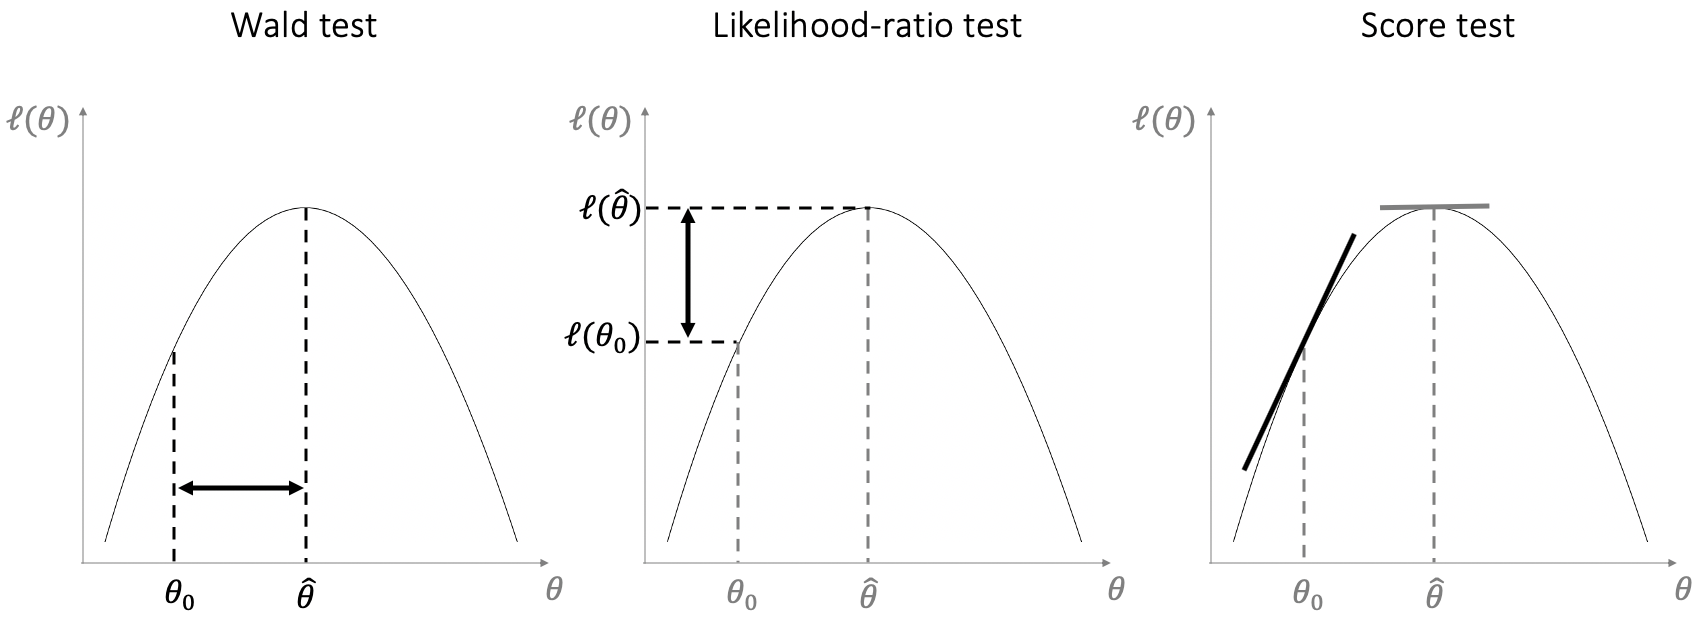
\includegraphics[width=15cm]{Chapter2/Fig/wald_lrt_score_tests.png}
\caption[Wald, LRT and Score test]{\textbf{The Wald test, the likelihood-ratio test and the Score test}.\\
The three most commonly used statistical testing approaches are illustrated here in the univariate case (single parameter $\theta$). 
On the x axis is the parameter $\theta$ on the y axis the log likelihood $\ell(\theta)$.
The Wald test essentially evaluates the difference between the \gls{mle} $\hat{\theta}$ and the parameter under $H_0$, $\theta_0$.
The likelihood-ratio test evaluates the difference between the log likelihoods evaluated at those values, i.e. $\ell(\hat{\theta})$ and $\ell(\theta_0)$.
Finally, the Score test evaluates the slope of $\ell(\theta)$ at $\theta_0$. Note that the slope at $\hat{\theta}$ is $=0$ by definition, as the MLE maximises $\ell(\theta)$.}
\label{fig:hypothesis_tests}
\end{figure}

\newpage

\subsubsection{Wald test}

First, let us consider the Wald test and the generic null hypothesis $H_0: \boldsymbol{\theta} = \boldsymbol{\theta}_0$ and the alternative $H_1: \boldsymbol{\theta} \neq \boldsymbol{\theta}_0$, where $\boldsymbol{\theta}$ are the parameters in our model and $\boldsymbol{\theta}_0$ are their values under $H_0$.
The Wald test statistic is defined as:

\begin{equation}\label{eq:Wald_test}
W = (\hat{\boldsymbol{\theta}}-\boldsymbol{\theta_0})^T [var(\boldsymbol{\theta_0})]^{-1}(\hat{\boldsymbol{\theta}}-\boldsymbol{\theta_0}), 
\end{equation}

where $\hat{\boldsymbol{\theta}}$ are the MLEs for the $\boldsymbol{\theta}$ parameters (values of $\boldsymbol{\theta}$ that maximise the likelihood).\\

% The XX theorem guarantees that, under some assumptions (ref),
It can be shown that, under some assumptions \cite{wald1943tests}, $W$ follows a chi-squared ($\chi^2$) distribution with number of degrees of freedom (dof) $d$ equal to the number of tested parameters ($W \sim \chi^2_d $).\\

In the univariate case (d = 1), eq. \eqref{eq:Wald_test} can be expressed as:

\begin{equation}\label{eq:Wald_test_univariate}
    W = \frac{(\hat{\theta}-\theta_0)^2}{var(\hat{\theta})} \sim \chi^2_1.
\end{equation}

Intuitively, the chance of rejecting $H_0$ increases as $\hat{\theta}$ is further away from $\theta_0$.
% and decreases as our confidence in the estimation of the \gls{mle} (i.e. $var(\hat{\theta})$) increases.

\newpage

\subsubsection{Likelihood ratio test}

Second, let's look at the \gls{lrt}.
% It was first introduced by XX. 
The test statistic in this case is the (log) likelihood ratio ($LLR$):

\begin{equation}\label{eq:log_likelihood_ratio}
LLR = \log \frac{L(H_1)}{L(H_0)} = \ell(H_1) - \ell(H_0). 
\end{equation}

Where we compare the value of the log-likelihood of the model under $H_0$ and under $H_1$, by evaluating eq. \eqref{eq:Linear_regression_log_likelihood} (or eq. \eqref{eq:Linear_regression_log_restricted_likelihood}) using MLE parameters estimated under $H_0$ ($\mathbf{0}$, $\sigma_0^2$) or $H_1$ ($\hat{\boldsymbol{\beta}}$, $\hat{\sigma_1^2}$).  \\

The Wilks theorem \cite{wilks1938large}, under some assumptions, guarantees that $2LLR$, too, follows a $\chi^2$ distribution with $d$ dof ($2LLR \sim \chi^2_d$).
The p value can then be calculated as:

\begin{equation}\label{eq:lrt_p_value}
    P(LLR) = 1-F_{\chi^2}(2LLR; d).
\end{equation}

\subsubsection{Score test}

Finally the Score test, also known as Lagrange multiplier test, is the last hypothesis test we consider. 
It was first developed by Rao in 1948 \cite{rao1948large}.
First, we define the score vector of Fisher as the gradient of the likelihood with respect to its parameters:

\begin{equation}\label{eq:score_vector}
    \mathbf{S} = \frac{\partial L}{\partial \boldsymbol{\theta}}.
\end{equation}

The Score test statistic is the Lagrange Multiplier (LM) and is defined as follows:

\begin{equation}\label{eq:lagrange_multiplier}
    LM = \mathbf{S}(\boldsymbol{\theta_0})^T [var(\boldsymbol{\theta_0})]^{-1}\mathbf{S}(\boldsymbol{\theta_0}). 
\end{equation}

It can be shown that $LM$, too, follows a $\chi^2$ distribution with $d$ dof ($LM \sim \chi^2_d$).

To understand the intuition behind this test let us consider again the univariate case (d = 1):

\begin{equation}\label{eq:lagrange_multiplier_univariate}
    LM = \frac{S(\theta_0)^2}{var(\theta_0)} \sim \chi^2_1.
\end{equation}

At the \gls{mle} $\hat{\theta}$, the log likelihood is maximised and therefore its gradient $S(\hat{\theta})$ is equal to $0$.
On the contrary, in principle, $ S(\theta_0) \neq 0 $ (Fig. \ref{fig:hypothesis_tests}). 
Intuitively, the further away from 0, the more likely we are to reject the null hypothesis.

\newpage

\subsubsection{Intuition on differences between LRT and Score test}

In this thesis, we apply both the \gls{lrt} and the Score test, for different applications.
I use this paragraph to highlight the key differences between the two tests and provide an intuition as to when one should use one or the other.
First of all, it can be shown that \cite{engle1984wald}:

\begin{equation}\label{eq:W_LLR_LM}
    W \geq LLR \geq LM.
\end{equation}

Let us exclude the Wald test for this purposes, eq. \eqref{eq:W_LLR_LM} guarantees that the log-likelihood ratio is always equal to or greater than the Lagrange multiplier.
As a consequence, the power  of the \gls{lrt}, defined as the probability of rejecting the null hypothesis when it is false: $P = P($reject $H_0 | H_1)$(see Box\ref{box:confusion_mat}) is the same or higher than the power of the Score test:

\begin{equation}
    (P_W \geq) P_{LLR} \geq P_{LM}.
\end{equation}

On the other hand, the false positive rate (FPR, Box\ref{box:confusion_mat}) of the \gls{lrt}, defined as the probability of rejecting the null hypothesis when it is true: FPR $= P($reject $H_0 | H_0)$ is also higher than the FPR of the Score test.
The Score test is therefore more accurate, making a smaller (or equal) number of Type I errors. 
One advantage of the \gls{lrt} is that it is robust to re-parametrisation of the parameters, whereas the Score test is not (for completeness, neither is the Wald test). 
On the other hand, one main advantage of the Score test is that it does not require the evaluation of the \gls{mle} of the parameters, but only evaluate the likelihood under the null hypothesis.
Finally, the LLR follows a $\chi^2$ distribution (asymptotically) only under the assumptions of the Wilks' theorem, which can be violated in certain applications.
Namely, the value of parameters tested should be far away from the boundaries of the possible values the parameter can assume.
For example, $-\infty < \beta < \infty$, so testing $H_1: \beta \neq 0$ satisfies the assumption.
On the other hand, $0 < \sigma^2 < \infty$ so testing $H_1: \sigma^2 \neq 0$ violates the assumption, because the value $0$ is right at the boundary.
Similarly, the Score test statistic does not follow a $\chi^2_1$ distribution in the presence of variance parameters, however an alternative test statistic can be defined which follows a linear combination of $\chi^2_1$ distributions, and efficient methods to evaluate its significance have been proposed by Davies \cite{davies1980algorithm}, Kuonen \cite{kuonen1999miscellanea} and Liu \cite{liu2009new, lee2012optimal}. \\

I will use the \gls{lrt} in the analyses in chapters 3-5, where the tests evaluate $\beta$.
I use Rao's Score test in chapter 6, where I will be evaluating the variance parameter $\sigma^2$.


\subsection{Multiple Testing Correction}
\label{sec:multiple_testing}

Hundreds of thousands or millions of variants may be individually tested within a typical human \gls{gwas}. 
In e\gls{qtl} mapping, we might test tens of thousands of genes, each essentially equivalent to a \gls{gwas} trait. 
Even when we only test for local e\gls{qtl} (in \textit{cis}, only SNPs within a window around the gene position, see section \ref{sec:eqtl}), we will still test hundreds of variants per gene, bringing the average number of tests performed well in the millions.  
When performing such a large number of tests, controlling single test p values results in a high number of false positives (for example, for p value < 0.01 and 10$^6$ tests we expect 10,000 false positives under the null hypothesis). 
This problem is known as the multiple hypothesis testing problem. 
In the next paragraphs, I give a brief overview of the methods commonly used in genetic analysis to correct for multiple hypothesis testing, with a focus on methods used in e\gls{qtl} mapping.

\subsubsection{Controlling family-wise error rate} 

One strategy to perform multiple testing correction is to control the probability of having at least one false positive for a trait, which corresponds to a trait-wise p value known as family-wise error rate (FWER, Box\ref{box:confusion_mat}).
The widely used Bonferroni method follows this strategy assuming independence between tests \cite{laird2010fundamentals}. 
Given a desired family-wise significance level $\alpha$, the method consists in calculating adjusted p values as $P_{adj} = P*n $, where n is the number of tests, and setting $P_{adj} < \alpha$ . 
This strategy ensures FWER < $\alpha$. 
The Bonferroni correction strategy is conservative, because of the assumption of independence between tests, which ignores correlations between genotypes due to \gls{ld}.\\

An alternative strategy, which accounts for the dependency of the statistical tests, is to use a permutation-based approach. 
The idea here is to is to build a background model by drawing from the empirical distribution maintaining the dependency structure of the underlying data but permuting the genotype data across individuals.
This way, we disrupt a possible association between phenotype and genotype whilst maintaining the overall dependencies.
For each association test (resulting in an observed p value $p_i$), we can perform the same test M times, each time considering a different permutation of the genotype data across individuals. 
The resulting p values $q_i,m$ represent the null distribution, i.e. the p values we might expect in the absence of any associations.

The p values from these M additional experiments are then used to calculate an adjusted p value, as the fraction of the M permutation p values that are lower than the observed p value. 

For test i, the experimental adjusted p value after M permutations is calculated as:

\begin{equation}\label{eq:permutation_adjusted_pvalue}
    P_{adj,i}^{perm} = \frac{1+\sum_{m=1}^{M} q_{i,m} \geq p_i}{1+M},
\end{equation}

where $q_{i,m}$ is the p value obtained at the m$^{th}$ permutation run equivalent to test i, and ones are added to avoid zero divisions.  
This strategy accounts for local \gls{ld}, thereby increasing the statistical power, and has been widely used in $cis$ molecular \gls{qtl} mapping to estimate gene-level p values \cite{gtex2015genotype, sudmant2015integrated}.  

% rephrase this
% Second, significant p values are truncated to a limited level of significance determined by the number of permutations. For example, 10,000 permutations restrict the p values to a lower bound of $10^{-4}$. Typically, one will obtain a list of genes that have the same lower-bound p values, such as $10^{-4}$. However, it is desirable to know the exact significance of each eGene p value for better interpretation and prioritization of genes.

However, as evident from eq. \eqref{eq:permutation_adjusted_pvalue}, the lower bound of $P_{adj,i}^{perm}$ depends on the number of selected permutations\footnote{For example, for M=1,000 the smallest adjusted p value we can obtain is only $P_{adj,i}^{perm}$=0.001 (when no permuted p value is smaller than the p value observed).} for which the test statistic is calculated, and thus a higher number of permutations may be required to estimate a p value with high enough accuracy \cite{sul2015accurate}.
This can be improved by increasing the number of permutations, e.g. using M as large as 100,000, but that entails a great computational burden and can become unpractical in molecular analyses of large cohorts.\\

Recently, one method has been developed that uses permutation results for as little as (M=) 50-100 permutations to estimate a full distribution of background permuted p values, allowing to exploit the benefits of the assumption-free permutation approach without too much of the computational burden \cite{ongen2016fast}. 
This is the method I will use in chapters 3-5 of this thesis to control for FWER at gene level when performing large scale \gls{eqtl} mapping.

\subsubsection{Controlling false discovery rate}

An alternative solution for multiple testing correction is to control the \gls{fdr}, i.e. the expected percentage of false discoveries (Box\ref{box:confusion_mat}).
The most widely used FDR-based correction method is the Benjamini-Hochberg (BH) procedure \cite{benjamini1995controlling}, which again assumes independence between tests. 
Let us consider T tests with p values $p_1, p_2, ..., p_T$ and let $r_1, r_2, ..., r_T$ be their ranks (the smallest p value has rank 1, the largest has rank T), defining adjusted p values as $P_{adj,i} = \frac{T*p_i}{r_i} $ and setting $P_{adj,i} <\alpha$ ensures FDR < $\alpha$.
Alternatively, the Storey procedure (proposed in 2002 \cite{storey2002direct}) optimises the BH procedure by taking into account the distribution of the p values in the experiment.
FDR corrected p values using the Storey procedure are sometimes called "q values".\\

% add intuition behind FWER/FDR?

For \gls{eqtl} mapping, the assumption of independent tests holds when we consider a single \gls{snp} per gene.
In this case, the number of tests T coincides with the numbers of genes tested.
In practice, in most applications one is interested in the lead \gls{snp} for each gene, i.e. the \gls{snp} corresponding to the minimum p value.
Conditional analyses (where we include the top \gls{snp} as a covariate in the model) can be used subsequently to detect secondary and tertiary effects for a gene.

\subsubsection{Multiple testing correction for \textit{cis} e\gls{qtl} mapping}

A typical strategy to correct for multiple hypothesis testing in molecular \textit{cis}-\gls{qtl} mapping is to use a two-step procedure \cite{gtex2015genotype}. 
First, for each gene an experiment-wise p value is obtained by correcting for multiple testing across variants using a FWER-based method. 
These gene-level p values are probability values for the hypothesis of a gene having at least one e\gls{qtl} in the analysed region (i.e. of being an eGene). 
Second, the gene-level p values are corrected to control the FDR, for example using the Benjamini-Hochberg procedure.\\

In the analyses in chapters 3-5 of this thesis, I adopt this two step approach.
I use M=1,000 permutations and the method described in \cite{ongen2016fast} to correct p values at the gene level (I will call the p values obtained this way "empirical feature p values").
Then, I select the top \gls{snp} per gene and correct the corresponding empirical feature p values a second time, using the Storey procedure \cite{storey2002direct}.
I will call the resulting p values: "globally corrected p values".

\subsection{Confounding effects in linear model}

The model in eq.\eqref{eq:Linear_regression_genetics} models the \gls{snp} tested as the only factor affecting the measured phenotype.
However, if available, additional relevant information for the samples tested (such as the sex or the age of the individuals) can be added to the model as covariates $\mathbf{W}$, and often improve the model:

\begin{equation}\label{eq:Linear_regression_genetics_covariates}
 \mathbf{y} =  \mathbf{W}\boldsymbol{\alpha} + \mathbf{g}\beta + \boldsymbol{\psi}, 
\end{equation}

where $\mathbf{W}$ is a NxP matrix whose the columns are known covariates and $\boldsymbol{\alpha}$ is a Px1 cevtor containing the corresponding weights.

Covariates are implemented as fixed effects (FEs), and they only contribute to the mean value of $\mathbf{y}$, such that $E[\mathbf{y}] = \mathbf{W}\boldsymbol{\alpha} + \mathbf{g}\beta$, while $Cov(\mathbf{y}) = Cov(\boldsymbol{\psi}) = \sigma_n^2 \mathbf{I_N} $, as before.
In some cases, we can add fixed effect covariates to control for other confounding, such as technical batches and other experimental conditions that might skew the results. \\

In \gls{eqtl} mapping, we can often take advantage of the expression profiles across all genes to identify global confounding affecting gene expression, even when we do not necessarily know the origin of the confounding.
For example, we can perform principal component analysis (PCA) on the full expression matrix (genes x samples) and include the first 10, 20 or 50 PCs as covariates in the model.
Alternative more sophisticated methods to compute factors capturing global trends are, among others, probabilistic estimation of expression residuals (PEER) \cite{stegle2010bayesian, stegle2012using} and multi-omics factor analysis (MOFA) \cite{argelaguet2018multi}. 

\subsection{Calibration studies and distributions of p values}

Under the assumption of no association between genetic variants and the analysed trait, an association model is expected to produce approximately uniform p values.
If that is the case, the model is said to be calibrated.
To verify that a model is calibrated we can disrupt the association between genotypes and phenotypes, by randomly permuting the genotypes. 
A representation that is often used to compare the observed (permuted) and the expected distributions of p values is the \gls{qq} plot. 
In a \gls{qq} plot the observed $-\log_{10}$(p value) is plotted against the expected $-\log_{10}$(p value), where the expected value is obtained by drawing from a uniform distribution. 
As confounding factors may create spurious associations, inflated \gls{qq} plots are typically associated with the presence of confounding and can be used as a diagnostic tool (Fig. \ref{fig:qqplots}). 

\vspace{2mm}

\begin{figure}[h]
\centering
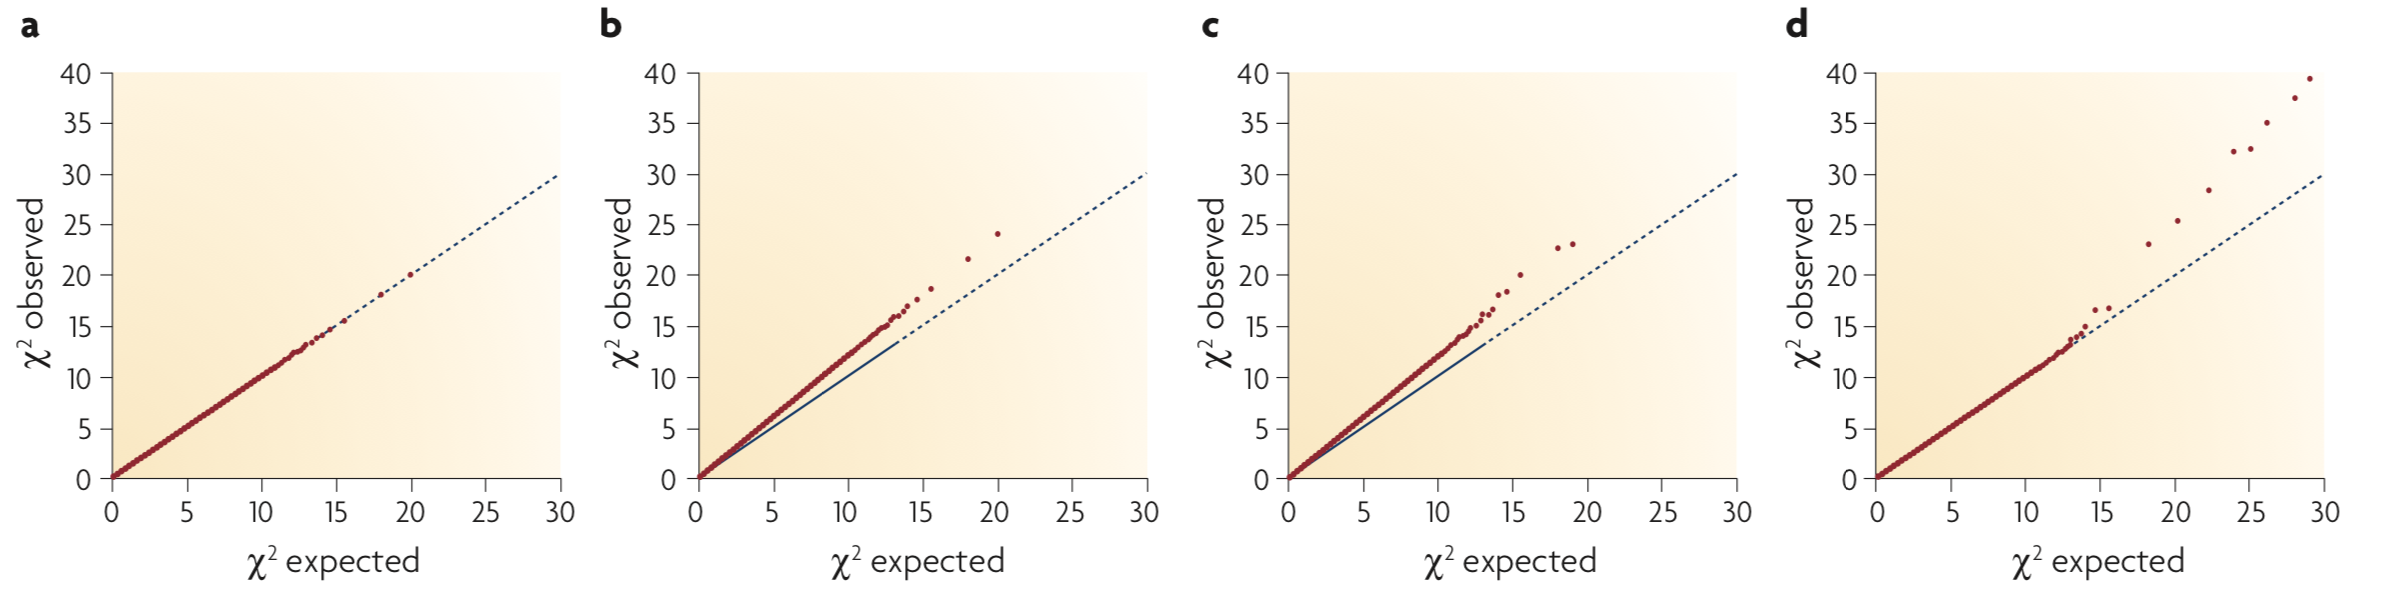
\includegraphics[width=15cm]{Chapter2/Fig/qqplots.png}
\caption[QQplots]{\textbf{QQplots}.\\
Placeholder adapted from \cite{mccarthy2008genome}
(a) no association (b) cryptic relatedness (c) population stratification (d) genuine association - change this to real data and $-\log_{10}$(p value) rather than $\chi^2$.}
\label{fig:qqplots}
\end{figure}


%********************************** %Third Section  **************************************

\section{Population structure and linear mixed models}
\label{sec:linear_mixed_models}

One major source of confounding effects in genetic analysis - that I have purposefully left out so far -  is latent population substructure, which includes population stratification (the presence in the study sample of individuals with different ancestral and demographic histories) and relatedness between individuals, both known and cryptic (evidence that individuals in the study sample have residual, non-trivial degrees of relatedness) \cite{mccarthy2008genome}.
It was acknowledged, even before the first \gls{gwas} was conducted, that there was a possibility of identifying false positives (or that true positives may be masked) when using population based association studies (instead of family based linkage studies), due to those confounding effects \cite{burton2005key}. 
This is because both phenotypic prevalence (proportion of individuals exhibiting the phenotype) and allele frequencies (frequencies of a specific allele within a population) vary across different populations, which may result in the identification of spurious association between variants and the phenotype of interest due to ethnicity or population sub-structure \cite{burton2005key}.

% name examples

\subsection{Approaches to account for population structure}
\label{sec:pop_struct_noLMM}

Various approaches have been proposed to account for population structure.
An early solution was genomic control \cite{devlin1999genomic}.
Genomic control correction adjusts for inflation by dividing the test statistic of each marker by the genomic control parameter ($\lambda_{GC}$\footnote{$\lambda_{GC}$ compares the test-statistic value with the median value, such that $\lambda_{GC} \approx 1$ means there is no evidence for confounding, $\lambda_{GC} \gg 1$ indicates that the presence of confounding is likely.}). 
However, as different markers have different abilities to differentiate across populations, this uniform adjustment is far from optimal. 
Indeed, the test statistic of markers that strongly segregate across populations may only be partially corrected, while the test statistic of markers that do not segregate may be over-corrected \cite{marchini2004effects, price2006principal}.

Alternatively, a method that attempts to correct the underlying problem is STRUCTURE, which assigns individuals to discrete populations subgroups and then combines the evidence for association across the different subgroups \cite{pritchard2000inference}. 
A limitation of this method is that only discrete subgroups can be considered. 
Additionally, it does not scale with sample size and is also highly sensitive to the number of defined population clusters \cite{price2006principal}.\\


Analyses of genotype data in larger cohorts, made possible by the advances in
genotyping technology, showed that genome-scale genetic variation could be used to
accurately infer population structure 
% Bauchet 2007, Jakobsson 2008, 
\cite{li2008worldwide, tian2008analysis, price2008discerning}.
In particular, the first principal components (PCs) of the genotype data were shown to correlate with orthogonal geographic axes
% lao 2008
\cite{novembre2008interpreting}.

As a result, one approach to account for population structure is to add the first genotypic PCs as covariates in the model (or to regress them out \cite{price2006principal}): 

\begin{equation}\label{eq:LM_PC_confounding}
    \mathbf{y} =  \mathbf{W}\boldsymbol{\alpha} + \sum_{i=1}^{p} PC_i b_i + \mathbf{g}\beta + \boldsymbol{\psi}. 
\end{equation}

The number of leading PCs p can be determined as the number of \gls{pc}s that cumulatively describe a certain proportion of the total variance.
% , or ..

This approach (eq. \eqref{eq:LM_PC_confounding}) was shown to perform relatively well in removing global population structure, but often failed to detect relatedness effects.
Therefore, when PCs are used to correct for population structure, closely related individuals have to be removed from the association analyses, prior to PCA calculations.
Even then, cryptic relatedness might still be present and would not be properly accounted for by this method. 

\subsection{Linear mixed models for genetic analyses}
\label{sec:LMM}

Alternatively, \gls{lmm}s can be used to successfully account for confounding effects linked to both population structure and relatedness 
% zhao 2007 , 
\cite{yu2006unified, kang2008efficient,kang2010variance, price2010new, zhou2012genome, lee2018genome}.
Instead of calculating principal components, the genotype data is used to estimate an NxN kinship matrix, $\mathbf{K}$, that describes the genetic similarity between pairs of individuals (see section below for a description of commonly used approaches to generate $\mathbf{K}$). 
This genetic similarity is modelled through the use of an additional random
effect term in the linear model described by eq. \eqref{eq:Linear_regression_genetics_covariates}, as follows:

\begin{equation}\label{eq:Linear_mixed_model}
 \mathbf{y} =  \mathbf{W}\boldsymbol{\alpha} + \mathbf{g}\beta + \mathbf{u} + \boldsymbol{\psi}, 
\end{equation}

where $\mathbf{u} \sim N(\mathbf{0}, \sigma_g^2\mathbf{K})$.
The use of the notation $\mathbf{K}$ signifies the fact that this matrix reflects a degree of "kinship" between individuals. 
It can be shown that the LMM approach is theoretically equivalent to the PC
approach when all PCs are regressed or included as covariates (see Hoffman \textit{et al.} \cite{hoffman2013correcting} for details), explaining why LMMs are able to account for more subtle population structure than the PC approach. 
However, regressing all PCs or including all PCs as covariates is not feasible in practice.




% The model in eq. \eqref{eq:Linear_mixed_model} can be alternatively expressed as:

% \begin{equation}\label{eq:LMM_MVN}
%  \mathbf{y} \sim  N(\mathbf{W}\boldsymbol{\alpha} + \mathbf{g}\beta, \sigma_g^2\mathbf{K} + \sigma_n^2\mathbf{I}).
% \end{equation}

% Note that for ease of notation in the following equations I have dropped the subscript $N$ from the identity matrix (i.e. $\mathbf{I} = \mathbf{I}_N$).

% Ideally, if we knew the underlying sub-population structure of our samples and could pinpoint which variants showed different allele frequencies within the population of interest, we could simply include such variants as covariates (i.e. similar to $\mathbf{W}$ from eq. \eqref{eq:Linear_regression_genetics_covariates}:

% \begin{equation}\label{eq:LM_G_confounding}
%     \mathbf{y} =  \mathbf{W}\boldsymbol{\alpha} +  \mathbf{G}_{conf}\mathbf{b}_{conf} + \mathbf{g}\beta + \boldsymbol{\psi}, 
% \end{equation}

% where $\mathbf{G}_{conf}$ is a matrix with columns corresponding to the genotypes of the \gls{snp}s whose frequencies vary within a population and thus cause confounding effects, and $\mathbf{b}_{conf}$ are the corresponding weights. 
% However, this is not typically the case.
% In fact, Fisher's work showed that it is the infinitesimal additions of a large number (if not all) of genetic variants that contributes to population structure \cite{fisher1919xv} .



% Alternatively, \gls{lmm}s can be used to successfully account for confounding linked to latent population structure.
% The intuition is to consider eq. \eqref{eq:LM_G_confounding}, but this time considering \gls{snp}s from the whole genome, since we do not know the "confounding variants":

% \begin{equation}\label{eq:polygenic_model}
%     \mathbf{y} =  \mathbf{W}\boldsymbol{\alpha} +  \mathbf{G}\mathbf{b} + \mathbf{g}\beta + \boldsymbol{\psi}.
% \end{equation}

% This is called the "polygenic model" (ref).
% Now, if we assume that the weights $\mathbf{b}$ are drawn from a common normal distribution $\mathbf{b} \sim N(\mathbf{0},\sigma^2_g\mathbf{I_M})$, where $M$ is the total number of \gls{snp}s, it can be shown that:

% \begin{equation}\label{eq:LMM_u_confounding}
%     \mathbf{u} =  \mathbf{G}\mathbf{b} \sim N(\mathbf{0},\sigma^2_g, \mathbf{G}\mathbf{G}^T)
% \end{equation}

% where $\mathbf{u}$ is a random variable which captures the effect of latent population structure onto $\mathbf{y}$.
% The model we just described is a \gls{lmm}.\\

% In terms of removing effects of population stratification, \gls{lmm}s have been shown to perform exactly as well as  including all M PCs (or regressing them out, \cite{price2006principal}), which is of course not feasible in practice.
% Additionally, \gls{lmm}s successfully correct for more subtle effects due to cryptic relatedness.
% However, \gls{lmm}s are typically much more computationally demanding.
% The next section describes \gls{lmm}s in general and introduces fast implementation approaches for a specific class of \gls{lmm}s.

% \subsection{Linear mixed models}

% % gwas reference: \cite{bush2012genome}

% In a \gls{lmm} the outcome variable can be described as a sum of deterministic effects (fixed effects, FE) and random effects (RE).
% % A random effect is ..
% A \gls{lmm} can be expressed as:

% \begin{equation}\label{eq:Linear_mixed_model_general}
%  \mathbf{y} =  \mathbf{W}\boldsymbol{\alpha} + \mathbf{Z}\mathbf{b} + \boldsymbol{\psi}, 
% \end{equation}

% where $\mathbf{y}$ is the outcome variable, $\mathbf{W}$ and $\mathbf{Z}$ are the design matrices of fixed and random effects respectively; $\boldsymbol{\alpha}$ are the fixed effects, $\mathbf{b} \sim N(\mathbf{0},\sigma_b^2\boldsymbol{\Sigma_b})$, $\boldsymbol{\Sigma_b}$ is a known covariance matrix, $\boldsymbol{\psi} \sim N(\mathbf{0},\sigma_n^2\mathbf{I})$ is the noise vector and $\sigma_b^2$ and $\sigma_n^2$ are the variance parameters of the random effect and the noise, respectively.\\

% In contrast to the case of linear regression discussed in section \ref{sec:linear_regression}, there is no close-form solution for the (restricted) \gls{mle} of the model parameters. \\

% However, for the model in eq. \eqref{eq:LMM_u_confounding} (i.e. when $\boldsymbol{\Sigma_b}$ factors as $\mathbf{G}\mathbf{G}^T$) it is possible to speed up computations, provided that we can perform feature selection on genomic variants and therefore make the genetic relatedness matrix low rank \cite{lippert2014greater}: 



\subsubsection{Kinship matrices}
\label{sec:kinship_matrices}

The covariance matrix $\mathbf{K}$ captures the latent population substructure of the study samples, including population stratification and genetic relatedness.
A few approaches have been proposed to compute this matrix, which is sometimes called the genetic relatedness matrix (GRM).\\

Fisher’s work \cite{fisher1919xv} shows that under an additive model with an infinite number of infinitesimal genetic effects, the phenotype is normally distributed and the phenotypic correlation between individuals is proportional to the fraction of genetic material that is identical-by-descent (IBD)\footnote{A locus is IBD in two individuals if it has been inherited by a common ancestor.}. 
Therefore, a natural way of defining the genetic relatedness between two individuals is to use the predicted proportion of the genome that is IBD in the considered pair. 
Historically, these IBD relatedness matrices were estimated from known pedigrees \cite{lange1976extensions}. 
Note that the definition of IBD requires the specification of a base population (i.e. the population of the ancestors, whose average relationship is zero), which in the case of pedigree designs is the population of the founders \cite{powell2010reconciling}.\\

An alternative that is becoming increasingly common is to estimate relatedness matrices from genome-wide SNPs. 
SNP-based relatedness matrices have been shown to improve narrow-sense heritability estimates \cite{visscher2006assumption, visscher2007genome, hayes2009increased} and to better account for population structure \cite{kang2008efficient, lee2010using} compared to pedigree-based matrices. 
Different ways of estimating relatedness matrices from genotype data have been proposed \cite{oliehoek2006estimating, purcell2007plink, vanraden2008efficient}. 
A widely-used estimate of the genetic relatedness matrix is the realised relatedness matrix (RRM) \cite{hayes2009increased}, which is defined as:

 \begin{equation}
    \mathrm{RRM} = \frac{1}{M}\mathbf{G}\mathbf{G}^T,
\end{equation}

where $\mathbf{G}$ is the NxM genotype matrix with standardised genotypes across individuals and M denotes the number of genome-wide variants. 
Interestingly, the RRM can be obtained from the polygenic model (where many or all genotypes contribute to the trait):

\begin{equation}\label{eq:polygenic_model}
    \mathbf{y} \sim N (\mathbf{W}\boldsymbol{\alpha} +  \mathbf{G}\mathbf{b}, \sigma_e^2\mathbf{I}),
\end{equation}

where $\mathbf{b}$ is an Mx1 vector containing the weights corresponding to $\mathbf{G}$ defined as above (standardised genotype matrix).
If we assume that $\mathbf{b}$ is drawn from a normal distribution such that: $\mathbf{b} \sim N(\mathbf{0}, \frac{\sigma_g^2}{M} \mathbf{I_M})$\footnote{Note that each genetic marker explains on average variance $\frac{\sigma_g^2}{M}$, so that genome-wide variants jointly explain variance $\sigma_g^2$.}, and marginalising out the random effect we obtain the RRM in one of the terms of the covariance:

\begin{equation}\label{eq:polygenic_model_MVN}
    \mathbf{y} \sim N (\mathbf{W}\boldsymbol{\alpha}, \sigma_g^2\frac{1}{M}\mathbf{G}\mathbf{G}^T + \sigma_e^2\mathbf{I} ),
\end{equation}

The RRM can also be interpreted as an IBD relatedness matrix where the base population
is the current population \cite{powell2010reconciling}.

Throughout this thesis, we use the RRM described in \cite{yang2011gcta} as implemented in plink \cite{purcell2007plink}.

% Hayes et al. 74 


% \subsubsection{Relationship to PCs}

% Principal components of the genotype data G can be calculated as the eigenvectors of the relatedness matrix $\mathbf{K} = \frac{1}{M}\mathbf{G}\mathbf{G}^T$\cite{price2006principal}. 
% Denoting with $\mathbf{Q}\mathbf{S}\mathbf{Q}^T$ the eigenvalue decomposition6 of $\mathbf{K}$, the marginalised model in eq. \eqref{eq:polygenic_model_MVN} can be obtained from the linear mixed model

% \begin{equation}
%     \mathbf{y} \sim N (\mathbf{W}\boldsymbol{\alpha} +  \mathbf{U}\mathbf{b}, \sigma_e^2\mathbf{I}),
% \end{equation}

% with $\mathbf{b} \sim N(\mathbf{0}, \sigma_g^2\mathbf{S})$
% by integrating out the random effects $\mathbf{b}$. 
% In summary, while a PC-based linear model only accounts for the first principal components of the genotype data using fixed effects, linear mixed models consider all the principal components using random effects. 
% This explains why LMMs can account for more subtle (i.e. high-rank) confounding compared
% to PC-based linear models. For further details on the relationship between PC-based
% models and random effect models I refer to Hoffman \cite{hoffman2013correcting}.

\subsection{Fast implementation of LMMs}

The biggest limitation of the use of LMMs for association studies is that they are in general very computationally intensive.
Computations associated with inference in linear mixed models scale cubically with
the number of individuals in the dataset. 
Indeed, for the generic LMM
the evaluation of the (restricted) marginal likelihood entails the computation of operations with $\mathcal{O}(N^3)$ complexity, specifically the inversion and the log determinant of the total covariance.% remove if add the following
% :

% \begin{equation}
%     \mathbf{y} \sim N(\mathbf{X}\boldsymbol{\beta}, \mathbf{K_{\theta}})
% \end{equation}

% (where $\mathbf{K_{\theta}}$ etc), 
% the evaluation of the restricted marginal likelihood:

% \begin{equation}
%     L = - \frac{N-F}{2} \log (2\pi) - \frac{1}{2} \log \det \mathbf{K_{\theta}} - \log \det \mathbf{X}^T\mathbf{K_{\theta}}^{-1}\mathbf{X}
% \end{equation}

% where $\boldsymbol{\beta}_{\theta} = (\mathbf{X}^T\mathbf{K_{\theta}}^{-1}\mathbf{X})^{-1}\mathbf{X}^T\mathbf{K_{\theta}}^{-1}\mathbf{y}$\\

% entails the computation of operations with $\mathcal{O}(N^3)$ complexity, specifically the inversion and the log determinant of the total covariance.

However, for the model in eq. \eqref{eq:Linear_mixed_model}, i.e. when the covariance matrix is known (does not depend on any parameters), and which can be alternatively expressed as:

\begin{equation}\label{eq:LMM_MVN}
 \mathbf{y} \sim  N(\mathbf{W}\boldsymbol{\alpha} + \mathbf{g}\beta, \sigma_g^2\mathbf{K} + \sigma_n^2\mathbf{I}),
\end{equation}

it is possible to speed up computations \cite{kang2008efficient, kang2010variance, lippert2011fast, zhou2012genome} enabling applications to large cohorts. 

These strategies reduce the computational complexity from $\mathcal{O}(N^3)$
per-variant to a single  $\mathcal{O}(N^3)$ cost up-front and a per-variant complexity of  $\mathcal{O}(N^2)$.
The complexity can be further reduced to $\mathcal{O}(N^2)$ for the up-front computation and a per-test complexity of  $\mathcal{O}(N)$, provided the genetic relatedness matrix is low-rank. \\
% In practice, this can be achieved through a feature selection approach, selecting a small proportion of all genome-wide variants to estimate $\mathbf{K}$ \cite{listgarten2012improved} or by randomly selecting a subset of the genome-wide variants. 



% As I will show in Section 2.3.3, an efficient derivative-free inference scheme can be used for association testing in univariate models 
% % \cite{}. 
% However, the number of variance parameters in variance component analyses and multi-trait models is typically too large for the efficient use of derivative-fee methods. 

% Multiple optimisation schemes have been proposed to optimise the restricted marginal likelihood in these cases

% However, in recent years, a lot of research has focused on methods to improving the efficiency of these methods.
% Whilst naively the LMM scales cubically with the number of samples, there are now methods available that scale linearly with the number of samples, once some up front computations that scale quadratically with the number of samples have been performed.
% These include FaST-LMM \cite{lippert2011fast}, BOLT-LMM \cite{loh2015efficient} and LIMIX \cite{lippert2014limix}, the latter built using a flexible framework such that different types of testing procedure can be easily and efficiently implemented, including interaction tests (see section \ref{sec:lmm_gxe}).\\
% FaST-LMM, BOLT-LMM, LIMIX.

% , including first-derivative methods, such as expectation maximisation (EM, Dempster et al., 1977) and its improved version PX-EM (Liu et al., 1998; Foulley and Van Dyk, 2000), and second-derivative methods, such as the Newton-Ralphson algorithm (Zhou and Stephens, 2014), the average information REML algorithm (Gilmour et al., 1995) and the Broyden’s method (Groeneveld, 1994). In this thesis, we follow (Groeneveld, 1994) and consider the Broyden’s method for parameters inference. 

% For a discussion on the different optimisation algorithms for inference in \gls{lmm}s, I refer to the supplementary information of Loh et al. (2015a).

I use this section to  briefly describe the efficient FaST-LMM algorithm proposed by Lippert \textit{et al} \cite{lippert2011fast}.
This is the algorithm implemented within the LIMIX toolset \cite{lippert2014limix,casale2015efficient} which I use throughout this thesis.\\


% ??

The intuition is to project all data into a space where phenotypic variables ($\mathbf{y}$) and covariates ($\mathbf{W}, \mathbf{g}$) are uncorrelated so that the model of the rotated data can be solved in closed-form.
% , i.e. with a diagonal covariance matrix. 
To do so, we perform eigen decomposition of $\mathbf{K}$ from eq. \eqref{eq:LMM_MVN}, such that: $\mathbf{K} = \mathbf{Q}\mathbf{S}\mathbf{Q}^T$, where $\mathbf{S}$ is a diagonal matrix containing the eigenvalues of $\mathbf{K}$ on the diagonal and 0s elsewhere, and $\mathbf{Q}$ is orthonormal ($\mathbf{Q}\mathbf{Q}^T = \mathbf{I}$), with columns corresponding to the eigenvectors of $\mathbf{K}$. \\

Then, if we define $\delta = \sigma_n^2/\sigma_g^2$ and consider it fixed, the full covariance matrix can be expressed as:

\begin{equation}\label{eq:fast_lmm_full_covariance}
 Cov(\mathbf{y}) = \sigma_g^2\mathbf{K} + \sigma_n^2\mathbf{I} = \sigma_g^2(\mathbf{Q}\mathbf{S}\mathbf{Q}^T + \delta\mathbf{I})= \sigma_g^2\mathbf{Q} (\mathbf{S} + \delta\mathbf{I})\mathbf{Q}^T.
\end{equation}

\vspace{4mm}

To simplify notation, we use $\boldsymbol{\Sigma} = \mathbf{K} + \delta\mathbf{I}$ and $\mathbf{X} = [\mathbf{W}, \mathbf{g}$], $\boldsymbol{\beta} = [\boldsymbol{\alpha}, \beta]$ so we can express the full log likelihood as:

\begin{equation} \label{eq:fast_lmm_log_likelihood}
 \ell(\boldsymbol{\beta}, \sigma_g^2, \delta) = -\frac{1}{2} \bigg\{N\log(2\pi\sigma_g^2) + \log{|\boldsymbol{\Sigma}|}+ \frac{1}{\sigma_g^2}(\mathbf{y}-\mathbf{X}\boldsymbol{\beta})^T\boldsymbol{\Sigma}^{-1}(\mathbf{y}-\mathbf{X}\boldsymbol{\beta}) \bigg\}. 
\end{equation}

Now the two expensive operations computationally are the inverse of the covariance matrix $\boldsymbol{\Sigma}$ (i.e. $\boldsymbol{\Sigma}^{-1}$) and its determinant ($|\boldsymbol{\Sigma}|$). 
Both can be solved efficiently as follows:  

\begin{equation}\label{eq:fast_lmm_Sigma_inverse}
    \boldsymbol{\Sigma}^{-1} = [\mathbf{Q} (\mathbf{S} + \delta\mathbf{I})\mathbf{Q}^T]^{-1} = \mathbf{Q} (\mathbf{S} + \delta\mathbf{I})^{-1}\mathbf{Q}^T = \mathbf{Q} \mathbf{D_{\delta}}\mathbf{Q}^T,
\end{equation}

where we we define $\mathbf{D_{\delta}}=(\mathbf{S} + \delta\mathbf{I})^{-1}$ which is a diagonal matrix whose i$^{th}$ element is: $\frac{1}{S_{ii} + \delta}$ and use the property of orthonormality of $\mathbf{Q}$ ($\mathbf{Q}^{-1} = \mathbf{Q}^T$).
As a result, this operation can be computed in linear time $\mathcal{O}(N)$.

\begin{equation}\label{eq:fast_lmm_Sigma_determinant}
    |\boldsymbol{\Sigma}| = |\mathbf{Q} (\mathbf{S} + \delta\mathbf{I})\mathbf{Q}^T|= |\mathbf{Q}||(\mathbf{S} + \delta\mathbf{I})||\mathbf{Q}^T| = |\mathbf{S} + \delta\mathbf{I}| = |\mathbf{D_{\delta}}^{-1}| = - |\mathbf{D_{\delta}}|,
\end{equation}

where we used the property of orthonormality of $\mathbf{Q}$ ($|\mathbf{Q}|=1$), and the determinant of a diagonal matrix ($|diag(\boldsymbol{\lambda)}| = \prod_{i=1}^{N} \lambda_i$) as well as properties of the logarithm\footnote{$\log |\mathbf{D_{\delta}}^{-1}|=\log |\mathbf{S} + \delta\mathbf{I}|=\log (\prod_{i=1}^{N} (S_{ii} + \delta))=\sum_{i=1}^{N} (\log (S_{ii} + \delta))=- \sum_{i=1}^{N} \frac{1}{\log (S_{ii} + \delta)}=-\log \prod_{i=1}^{N} \frac{1}{(S_{ii} + \delta)}=- \log |\frac{1}{\mathbf{S} + \delta\mathbf{I}}|=-\log |\mathbf{D_{\delta}}|$}.\\

% a bit of a gap here
We can now re-write the log-likelihood as:

\begin{equation}
    \begin{split}
        \ell(\boldsymbol{\beta}, \sigma_g^2, \delta) = -\frac{N}{2} \log(2\pi) -\frac{N}{2} \log(\sigma_g^2) + \frac{1}{2} \log|\mathbf{D_{\delta}}| - \frac{1}{2\sigma_g^2}(\mathbf{y}-\mathbf{X}\boldsymbol{\beta})^T\mathbf{Q}\mathbf{D_{\delta}}\mathbf{Q}^T(\mathbf{y}-\mathbf{X}\boldsymbol{\beta}) \\
        =  -\frac{N}{2} \log(2\pi) -\frac{N}{2} \log(\sigma_g^2) + \frac{1}{2} \log|\mathbf{D_{\delta}}| - \frac{1}{2\sigma_g^2}(\mathbf{Q}^T\mathbf{y}-\mathbf{Q}^T\mathbf{X}\boldsymbol{\beta})^T\mathbf{D_{\delta}}(\mathbf{Q}^T\mathbf{y}-\mathbf{Q}^T\mathbf{X}\boldsymbol{\beta}) \\
        =  -\frac{N}{2} \log(2\pi) -\frac{N}{2} \log(\sigma_g^2) + \frac{1}{2} \log|\mathbf{D_{\delta}}| - \frac{1}{2\sigma_g^2}(\tilde{\mathbf{y}}-\tilde{\mathbf{X}}\boldsymbol{\beta})^T\mathbf{D_{\delta}}(\tilde{\mathbf{y}}-\tilde{\mathbf{X}}\boldsymbol{\beta}),
    \end{split}
\end{equation}

where $\tilde{\mathbf{y}} = \mathbf{Q}^T\mathbf{y}$ and $\tilde{\mathbf{X}}= \mathbf{Q}^T\mathbf{X}$ are the rotated phenotype vector and covariate matrix (including the genotype vector $\mathbf{g}$).

If we consider $\delta$ fixed, the first and third terms are constant, so i can rewrite:

\begin{equation}
    \ell = const - \frac{N}{2} \log(\sigma_g^2) - \frac{1}{2\sigma_g^2}[\mathbf{D_{\delta}}^{\frac{1}{2}}\tilde{\mathbf{y}}-\mathbf{D_{\delta}}^{\frac{1}{2}}\tilde{\mathbf{X}}\boldsymbol{\beta}]^T[\mathbf{D_{\delta}}^{\frac{1}{2}}\tilde{\mathbf{y}}-\mathbf{D_{\delta}}^{\frac{1}{2}}\tilde{\mathbf{X}}\boldsymbol{\beta}].
\end{equation}

Then, we can compute $\hat{\boldsymbol{\beta}}$ and $\hat{\sigma_g^2}$ using eq. \eqref{eq:Linear_regression_MLE_solution_beta} and eq. \eqref{eq:Linear_regression_MLE_solution_sigma} for the linear model:

\begin{equation}
    \mathbf{D}^{\frac{1}{2}}_{\delta}\mathbf{Q}^{T}\mathbf{y} \sim N(\mathbf{D}^{\frac{1}{2}}_{\delta}\mathbf{Q}^{T}\mathbf{X}\boldsymbol{\beta}, \sigma_g^2\mathbf{I}).
\end{equation}


To further speed up computations, $\boldsymbol{\alpha}$ and $\delta$ are only optimised once, under $H_0$, which is the same for all \gls{snp}s for a given trait.
Since there is no closed-form for $\delta$, we use the numerical method Brent search to find the optimal $\hat{\delta}$ \cite{goddard2009estimating}.
For every \gls{snp}, we find the \gls{mle}s for $\beta$ and $\sigma^2_g$ using the closed-form from equations \eqref{eq:Linear_regression_MLE_solution_beta},\eqref{eq:Linear_regression_MLE_solution_sigma}.\\

When the rank of $\mathbf{K}$ is much smaller the number of individuals $rank(\mathbf{K}) << N$,  we can further speed up the algorithm by computing the "economical" eigen decomposition \cite{lippert2011fast}, where we use the fact the most eigenvalues of $\mathbf{K}$ are 0:

\begin{equation}\label{eq:economic_eigen_decomposition}
    \overbrace{[\mathbf{Q_0} \quad \mathbf{Q_1]}}^{\mathbf{Q}}
            \overbrace{\left[\begin{array}{cc}
                \mathbf{S_0} & \mathbf{0}\\
                        \mathbf{0} & \mathbf{0}
            \end{array}\right]}^{\mathbf{S}}
        \left[\begin{array}{c}
            \mathbf{Q_0}^T \\
            \mathbf{Q_1}^T
        \end{array}\right] = \mathbf{K}.
\end{equation}

For details on this implementation I refer the reader to the Supplementary note from \cite{lippert2011fast}.


\subsection{Linear mixed models for eQTL mapping}

When running fast \gls{lmm} in the context of \gls{eqtl} mapping, we run the model for each gene separately.
For a given gene, the model under $H_0$ is fixed.
Because we are performing \textit{cis} \gls{eqtl} mapping, we define a \textit{cis} window around the gene (typically ranging from 100 kilo-basepair to 1 Mega-basepair) and a minimum \gls{maf} (e.g. 0.05) and test all \gls{snp}s within the window with \gls{maf} > 0.05 in our population.  
We test one \gls{snp} at a time, and only the alternative model is changing.
This means that all weights $\boldsymbol{\alpha}$ excluding the SNP effect, and $\delta$ are only computed once per gene.\\

Typically, for each gene-\gls{snp} pair tested the reported values are i) the p value (e.g. obtained using eq. \eqref{eq:lrt_p_value}), ii) the estimated effect size $\beta$, and iii) the effect size standard error ($se(\beta)$).

% how is se(beta) computed?

Subsequently, multiple testing correction is applied, first at the gene level (using FWER) and then globally (using FDR, as described in Section \ref{sec:multiple_testing}).
The resulting adjusted p values are also reported.\\

To summarize a typical eQTL map, a number frequently reported is the number of genes with at least one \gls{eqtl} (from now on "eGenes"), often reported together (or as a fraction of) the number of genes tested. \\


% \subsection{\gls{lmm}s for variance component analysis}

% \subsubsection{heritability}

% \subsubsection{gene expression variance components}

% \newpage 

%********************************** %Fourth Section  **************************************

\section{Linear Mixed Models for GxE}
\label{sec:lmm_gxe}

The  statistical test described in section \ref{sec:hypothesis_testing} refers to an "association test" where we want to test for an effect that the \gls{snp} of interest has on a trait directly\footnote{Note that this was described for a linear regression but can be equivalently applied to the linear mixed model, i.e. $H_0: \mathbf{y} \sim N (\mathbf{0}, \sigma_g^2\mathbf{K} + \sigma_n^2\mathbf{I})$ vs $H_1: \mathbf{y} \sim N (\mathbf{g}\beta, \sigma_g^2\mathbf{K} + \sigma_n^2\mathbf{I})$, where the test assesses $\beta = 0$ vs $\beta \neq 0$.}.

However, the same \gls{lmm}s and fast implementation approaches described so far can be applied, with care to testing for genotype-environment (GxE) interactions instead (let us call this an "interaction test" for simplicity).\\

As described previously (section \ref{sec:gxe}), a significant statistical \gls{gxe} interaction is defined when there is a significant difference in the genetic effect between groups of individuals with different environmental exposures (Fig. \ref{fig:gxe}).

\begin{figure}[h]
\centering
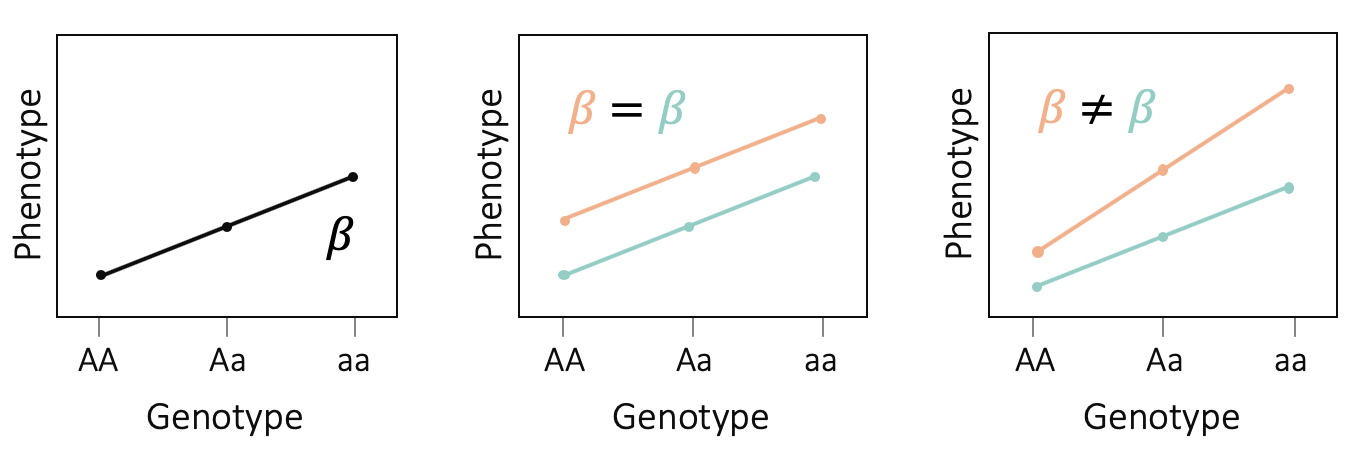
\includegraphics[width=15cm]{Chapter1/Fig/GxE.png}
\caption[Illustration of GxE]{\textbf{Illustration of GxE effect for two environmental groups}.\\
Illustrated are the mean phenotype values across three genotypic groups for a given locus (AA: homozygous minor allele, Aa: heterozygous individuals, aa: homozygous major allele).
The first plot (left) describes the case of a genetic effect of the variant on all individuals. 
$\beta$ represents the (in this case positive) effect size of the locus tested. 
The second plot (middle) shows that two groups of individuals characterised by different environmental exposure (represented by the colours). 
The environments have an effect on phenotype (as represented by a shift upwards for the orange group) but the genetic effect remains constant. 
Finally, the third plot (right) shows a GxE effect.
There is an interaction effect between the individuals' genotypes and their environmental exposure, such that for one group (orange) the genetic effect was exacerbated whilst for the other group (seagreen) the effect was dampened.}
\label{fig:gxe}
\end{figure}

In the following, I describe various approaches to test for GxE, which all build on the \gls{lmm} framework. 

\subsection{Stratified interaction test}

A possible way to detect interaction effects, is to stratify samples into discrete subgroups based on their environmental exposure.
In \gls{eqtl} mapping, one might for example cluster cells into cell types, or separate samples into different condition groups.
Then a LM (eq. \eqref{eq:Linear_regression_genetics_covariates}) or \gls{lmm} (eq. \eqref{eq:Linear_mixed_model}) can be applied to each stratum and the marginal variant effects can be compared to assess whether there is a significant difference in these effects across the sub-populations.
I will refer to this method as the "stratified interaction test".

However, as more detailed environmental data is collected, allowing for finer stratification of the population, these methods are no longer optimal as the sub-populations become too small to obtain stable estimates of the variant effects.
For example, as more and more rare cell types are identified and as the definition itself of cell types becomes more blurred, joint analyses become necessary.

% add reference to multi-tissue eqtl mapping methods

\subsection{Single environment interaction test}

A second commonly used method to test for interaction effects is an extension of the LM or \gls{lmm} to include two additional FE terms, an interaction term (GxE) and an environment term (E):

\begin{equation}\label{eq:Interaction_test_FE_LMM}
 \mathbf{y} =  \mathbf{W}\boldsymbol{\alpha} + \mathbf{e}\gamma  + \mathbf{g}\beta_G + \mathbf{e}\odot\mathbf{g}\beta_{GxE} + \mathbf{u} + \boldsymbol{\psi}, 
\end{equation}

where $\mathbf{e}$ represent the environment term, $\gamma$ is its corresponding weight and where two genetic effect terms are present, $\beta_G$ which is the "persistent" genetic effect size whilst $\beta_{GxE}$ is the effect of the interaction term (GxE).
Finally, $\odot$ denotes element-wise multiplication (Hadamard product).
The test is:

\begin{equation}
 H_{0}: \beta_{GxE}=0 
\end{equation}
vs
\begin{equation}
 H_{1}: \beta_{GxE} \neq 0. 
\end{equation}

This model allows to directly test for a GxE interaction effect with a certain environment/factor, beyond the additive effects of the \gls{snp}s and the environment themselves. 
Of course, the same model can also be extended to the case of multi-environment interaction by simply adding more environments as FE terms:

\begin{equation}\label{eq:multi_interaction_test_FE_LMM}
 \mathbf{y} =  \mathbf{W}\boldsymbol{\alpha} + \mathbf{e}_1\gamma_1 + \mathbf{e}_2\gamma_2 + ...  + \mathbf{g}\beta_G + \mathbf{e_1}\odot\mathbf{g}\beta_{GxE,1}+ \mathbf{e_2}\odot\mathbf{g}\beta_{GxE,2} + .. + \mathbf{u} + \boldsymbol{\psi}. 
\end{equation}

However, this becomes quickly infeasible for large numbers of environments, especially for relatively small sample sizes, because of the dof loss when increasing the number of parameters to estimate (two additonal parameters to estimate for every environment included).


\subsection{StructLMM}

A recently proposed method called StructLMM (structured linear mixed model) allows for the joint analysis of GxE effect of hundreds of environmental variables \cite{moore2019linear} in an efficient manner.
In Chapter 6, I will present an extension to StructLMM for applications to scRNA-seq data so I refer the reader to that chapter for derivations of the updated model.
Instead, I will use this section to give an intuition for the method.\\

The \gls{lmm} in eq. \eqref{eq:Linear_mixed_model} models the weight of a given \gls{snp} (or effect size, $\beta$) as a scalar, where the assumption is that the effect of a \gls{snp} on the trait is the same across all samples.
However, as we have seen, samples belonging to different environmental subgroups can have different effects of a \gls{snp} on a trait due to \gls{gxe} effects (Fig. \ref{fig:gxe}).
Moreover, the sub-grouping might be extremely complex, possibly driven by several environmental exposures, making adding them all in the model described in eq. \eqref{eq:multi_interaction_test_FE_LMM} infeasible.\\

The intuition of Struct\gls{lmm} is to again consider the \gls{snp} effect size as split into two components, the persistent effect size, which is assumed to be persistent across conditions (we call this $\beta_G$) and the GxE effect size. 
However, here the GxE effect size is modelled as a random variable and is a Nx1 vector ($\boldsymbol{\beta}_{GxE}$), which depends on the environmental structure of the samples:

\begin{equation}\label{eq:StructLMM-int}
 \mathbf{y} =  \mathbf{W}\boldsymbol{\alpha} + \mathbf{g}\beta_G + \mathbf{g} \odot \boldsymbol{\beta_{GxE}} + \mathbf{e} + \boldsymbol{\psi}, 
\end{equation}

where $\odot$ denotes Hadamard product, such that $\mathbf{g} \odot \boldsymbol{\beta_{GxE}} = diag(\mathbf{g})\boldsymbol{\beta_{GxE}}$ where $diag(\mathbf{g})$ is an NxN diagonal matrix, i.e. all off-diagonal elements are 0, diagonal elements correspond to elements of the Nx1 vector $\mathbf{g}$, whereas $\boldsymbol{\beta_{GxE}}$ is a Nx1 vector such that:

\begin{equation}\label{eq:StructLMM-int_beta_GxE}
    \boldsymbol{\beta_{GxE}} \sim N(\mathbf{0}, \sigma^2_{GxE}\mathbf{E}\mathbf{E}^T).
\end{equation}

Further, $\mathbf{e} \sim N(\mathbf{0}, \sigma^2_{e}\mathbf{E}\mathbf{E}^T)$ and $\boldsymbol{\psi} \sim N(\mathbf{0}, \sigma^2_{n}\mathbf{I})$. \\


The test then is:

\begin{equation}\label{eq:StructLMM-int_H0}
 H_{0}: \sigma^2_{GxE}=0 
\end{equation}
vs
\begin{equation}\label{eq:StructLMM-int_H1}
 H_{1}: \sigma^2_{GxE} \neq 0. 
\end{equation}\\

StructLMM also allows to test for associations, whilst accounting for GxE effects, essentially testing for any effects of a given variant, either G or GxE.
However, this is beyond the scope of this thesis so I refer the reader to the original paper \cite{moore2019linear}.\\

The main limitation of StructLMM is that for reasons of inference efficiency it does not properly account for population sub-structure.
Note that the term $\mathbf{e}$ in \eqref{eq:StructLMM-int} accounts for effects that the environmental sub-structure of individuals might have on the phenotype directly (i.e. not mediated by $\mathbf{g}$).
However, that leaves no room to account for genetic population sub-structure.
For unrelated individuals, as we discussed in section \ref{sec:pop_struct_noLMM}, it may be sufficient to include \gls{pc}s as covariates.
In the case of repeated samples, however, whether it is single cells from the same donor or longitudinal measures from the same individual, that is no longer the case.
In Chapter 6, I propose a solution for this problem and apply the model on a variety of simulated and real \gls{scrnaseq} datasets.



\section{Discussion}

Linear mixed models are widely applied in genetic association analysis because they offer great control for confounding effects.
Throughout this thesis, I will use different models for \gls{eqtl} mapping using single cell expression profiles, which all build on this framework.

I have used this chapter to lay the foundation and notation for which we build extensions in the coming chapters.

Specifically, in chapter 3 we provide a best practice pipeline for performing bulk-like \gls{eqtl} mapping using single cell data, where we test various aggregation methods as well as design matrices and then use the standard linear mixed model from eq. \eqref{eq:Linear_mixed_model}.
We compare our results to an \gls{eqtl} map obtained using bulk RNA-seq from the same samples and also compare results across scRNA-seq technologies for a subset of donors.

In chapters 4 and 5 we use different adaptions of linear and linear mixed models to test both for associations (eq. \eqref{eq:Linear_mixed_model}) and interactions (eq. \eqref{eq:Interaction_test_FE_LMM}). 

Finally, in chapter 6 we present scStruct-LMM, an extension to the StructLMM model (in eq. \eqref{eq:StructLMM-int}) that is able to handle repeated observations from the same samples.
The model is originally intended for single cell data, and allows to test for context-specific \gls{eqtl} mapping across cell contexts and states.
However, it could also be suited for performing GxE interactions across many variables in any other study with replicated measurements for the same individual, such as longitudinal studies for example.
%!TEX root = ../thesis.tex
%*******************************************************************************
%****************************** Third Chapter *********************************
%*******************************************************************************

% \chapter{Mean level eQTL mapping using single cell RNA-seq data from iPSCs}
\chapter{Comparison of eQTL mapping using bulk and single cell RNA-seq readouts}
\label{chapter3}

% abstract
As discussed in \textbf{section 
\ref{sec:eqtl}},
% 1.1.8}, 
in traditional 
eQTL
% \gls{eqtl}
mapping 
individual-level 
gene expression 
% profiles are 
is
measured using bulk RNA-sequencing, where 
the quantified 
% gene 
expression profiles represent
% expression level is averaged across 
several thousands of cells from each individual.
As we have seen, recent technological advances 
% in experimental techniques 
have allowed molecular phenotypes, including gene expression, to be assayed at the level of single cells.
In particular, 
scRNA-seq
% \gls{scrnaseq} 
% assays are now well established,
is now an established technique, 
and can be deployed at population-scale, across several individuals.
% and computational methods to analyse the data have become fairly standardised.
% with fairly standardised methods for performing both low-level analyses and complex tasks, such as clustering and pseudotime estimation.
Owing to their ability to identify cell types and cell states in a data-driven manner,
% no references in abstract?
% \cite{buettner2015computational},
% \gls{scrnaseq} 
scRNA-seq
data from a single experiment can be used to define homogeneous cell populations, quantify expression levels within them, and then map eQTL in each of them separately.
% - and then quantify expression levels within -  the use of \gls{scrnaseq} data, 
% combined with genotype information, 
% These types of analyses can improve
% % is uniquely positioned to provide an extra layer to 
% our understanding of the genetic regulation of expression, across
% % a plethora of 
% cell types and states.
As a consequence, studies where single cell expression profiles (rather than bulk) are used to perform
% \gls{eqtl}
eQTL
mapping 
% (where the effect of common genetic variants on expression is assessed at single cell resolution)
% \gls{scrnaseq} profiles are combined with genotype information to map \gls{eqtl})
% is quickly emerging as a field of research, 
have emerged recently, and promise
% and it promises 
to greatly improve our understanding of the genetic architecture of 
gene regulation
% human disease 
across tissues, in both human disease and development.
% However, the extent to which \gls{eqtl} identified using scRNA-seq data can replicate those obtained using the `gold standard' bulk RNA-seq approach has not been explored.
% However, there has not been a systematic comparison between single cell and bulk RNA-seq obtained eQTL maps to date.
However, the use of single-cell RNA-seq to map eQTL maps as opposed to using bulk RNA-seq profiling has not been systematically benchmarked.
% However, the relationship between eQTL maps obtained using single cell data as compared to bulk data has not been systematically explored.
To address this, here
% Here,
I select a very homogeneous cell type (iPSCs), where direct comparison is possible.
In particular,
% Here, 
I use matched bulk and single cell RNA-seq from over 100 human 
% \gls{ipsc} 
iPSC lines 
% donors
to assess our ability to detect 
% \gls{eqtl} 
eQTL
using single cell RNA-seq data, and the extent to which we can replicate 
% \gls{eqtl}
eQTL
identified using bulk RNA-seq, when mapping eQTL using a common analytical framework based on LMMs (see \textbf{Chapter 
% 2
\ref{chapter2}}).
% Direct comparison is possible in this system, given the very homogeneous cell type (iPSCs).
Additionally, for a subset of lines, I compare results using two different scRNA-seq technologies.
As more and more single cell-eQTL
% \gls{eqtl}
(sc-eQTL) studies emerge, I believe that
the insights presented here will help
% this is a useful step towards 
establishing a `best practice' workflow, to optimise yield of sc-eQTL
% \gls{eqtl}
maps and to establish uniform methods across the field.
% I show preliminary results where
% we systematically assess the role played by multiple factors including the chosen aggregation method and covariates used and compare results across technologies.
% We believe this is a useful resource for several future studies that will want to perform \gls{eqtl} mapping using single cell expression profiles.

\newpage

\begin{Comment2}
% \subsection{Contributions}
\hspace{-3mm}\textbf{Contributions} 
In this chapter, I present results from two main bodies of work.

First, I describe a set of results from analyses I have conducted in the context of a larger collaborative project between the Stegle, Marioni and Vallier labs. 
In particular, the data was generated by Ludovic Vallier’s lab at the Sanger Institute, and the experiments were led by Mariya Chhatriwala, using cell lines from the \gls{hipsci} project.
Davis McCarthy and I processed the scRNA-seq data and performed quality control.
Marc Jan Bonder processed the bulk RNA-seq data.
I performed all analyses presented in the first part of this chapter, under the supervision of Oliver Stegle and John Marioni.
% The text from which this chapter is based was written collaboratively by myself, John Marioni and Oliver Stegle.
The code for processing, analysing and plotting the data is open source and freely accessible here: \url{https://github.com/single-cell-genetics/singlecell\_endodiff\_paper}.\
The paper 
% \cite{cuomo2020single}
is available at \url{https://www.nature.com/articles/s41467-020-14457-z} and has been published as:\\

Anna S.E. Cuomo*, Daniel D. Seaton*, Davis J. McCarthy*, Iker Martinez, Marc Jan Bonder, Jose Garcia-Bernardo, Shradha Amatya, Pedro Madrigal, Abigail Isaacson, Florian Buettner, Andrew Knights, Kedar Nath Natarajan, the Hipsci Consortium, Ludovic Vallier, John C. Marioni, Mariya Chhatriwala, Oliver Stegle. Single-cell RNA-sequencing of differentiating iPS cells reveals dynamic genetic effects on gene expression. \textit{Nature Communications}, 2020, (* equal contribution)\\


In the second part of this chapter, I present more recent preliminary results from work in collaboration with Giordano Alvari and Marc Jan Bonder, from the Stegle lab.
This project was designed by Marc Jan Bonder and myself, to extend the results presented in the first part of this chapter.
Giordano performed most of the analyses, under mine and Marc Jan Bonder's supervision.
Marc Jan Bonder and I performed the remaining analyses and summarised the results.\\

I generated all figures included in this chapter, except where indicated otherwise in figure legends.
% between the Stegle, Bonder and McCarthy labs.
% The project was lead by Giordano Alvari under Marc Jan Bonder's supervision and mine.
% Christina Azodi supervised by Davis McCarthy performed the simulation analyses.
% \vfill
\end{Comment2}

\newpage

\section{Introduction}

As outlined in \textbf{section 
% 1.1.8},
\ref{sec:eqtl}} 
since the publication of the first human \gls{eqtl} map in 2003 \cite{schadt2003genetics}, the field has adapted to adopt technological advances as they emerged, both in terms of statistical approaches (from linkage analysis to genome-wide scans), and of new technologies for the estimation of gene expression (from microarrays to RNA-seq).
I use this section to give a brief overview of methods to estimate gene expression (\textbf{section \ref{sec:gene_expression}}), the advent of single cell RNA-seq (\textbf{section \ref{sec:scrnaseq}}) and the consequent birth of the (very new) single cell-\gls{eqtl} mapping field of research (\textbf{section \ref{sec:sc_eqtl}}). 

\subsection{Measuring gene expression}
\label{sec:gene_expression}

Early methods for estimating the number of expressed mRNA molecules associated with a particular gene (hereafter defined as a gene's expression)
% to estimate the RNA levels of genes 
were Northern blots \cite{alwine1977method} and quantitative reverse transcription polymerase chain reaction, qRT-PCR \cite{gibson1996novel}. 
In Northern blots, electrophoresis is used to separate RNA, which is then visualised by hybridisation with labelled probes. 
A key limitation of Northern blots is that they require large amounts of input material and the results are mostly only qualitative.
% , at most semi-quantitative.
In qRT-PCR, RNA is reverse-transcribed into complementary DNA (cDNA) and then amplified using PCR, after each cycle of which the concentration of DNA is measured using a fluorescent dye. 
This required normalisation relative to a standard gene (e.g. 
housekeeping genes, or 
ribosomal genes) which was assumed to be `stable', making this method also not very quantitative.
% both are low-throughput
Additionally, both of these methods were very low-throughput, typically used only to quantify one, or at most few genes - hence being referred to as `single gene approaches'.
% Additionally, these methods were not very accurate, as the quantification of each gene required normalisation relative to a standard gene
% of known sequence and quantity, called an RNA spike-in.
% \footnote{An RNA spike-in is an RNA transcript of known sequence and quantity used to calibrate measurements in RNA hybridisation assays.}. 
\\

In 1995, DNA microarrays were introduced \cite{schena1995quantitative}, which for the first time allowed the estimation of expression levels for many genes simultaneously.
Like qRT-PCR, microarrays rely on the reverse transcription of RNA into cDNA.
This cDNA is then labelled with a fluorescent dye and hybridised to a DNA microarray containing complementary DNA for thousands of known transcripts at specific locations. 
% JCM: spike-ins have not been defined. Also, differences between one and two colour array based technologies. I wouldn't go into this in depth, but this is perhaps a little too superficial here.
The RNA levels can then be estimated by measuring the intensity of fluorescence at each location and either normalising it using RNA transcripts of known concentration (called RNA spike-ins; `one colour array') or directly comparing it to a second sample on the same microarray using two different fluorescent dyes (`two colour array').
% Towards the end of the 20th century, 
Microarrays quickly became the most commonly used method for measuring gene expression levels. 
However, since microarrays only allow the measurement of RNA with a known sequence, they are not suitable for the detection of novel transcripts or alternative splice isoforms. 
% They are also often unable to measure the expression of transcripts with low abundance due to background noise (Gautier et al., 2004) and are not necessarily suitable for studying the absolute expression of genes in a single sample (Allison et al., 2006).
% \\

In the late 2000s, RNA sequencing (RNA-seq), based on next-generation sequencing (NGS), 
% of the c\gls{dna} allows for genome-wide quantification of the transcriptome.
was introduced.
RNA-seq allows for the direct sequencing and quantification of cDNA libraries \cite{mortazavi2008mapping} and has since been shown to be superior to microarrays in almost all regards 
% except cost
\cite{marioni2008rna}, as it provides information about a gene's sequence, in addition to its expression level.
In particular, in addition to the quantification of known transcripts, RNA-seq also enables the identification of completely new genes, previously unknown genetic variants in the genes, variation in alternative splicing, or post-transcriptional modifications (see also \textbf{section 
\ref{sec:eqtl_map}}).
% 1.1.8}). 
\\

In recent years, next generation sequencing approaches have been extended to quantify variation in RNA expression at single cell resolution, starting the `single cell RNA-seq era'.


% % Intro on molecular readouts as intermediate to understand genotype-phenotype mechanisms.
% % Going back in time to our progressive better understanding of molecular machinery, starting from Crick postulating the central dogma.

% % \subsection{Estimation of gene expression levels}

% % In this thesis, we focus on gene expression, i.e., the transcriptome, as a molecular phenotype.
% % In general, the transcriptome describes the complete set of transcripts in a tissue or cellular sample, and their respective quantity. 
% % As a precursor of protein expression, mRNA can serve as a proxy of gene expression levels. 
% % Multiple approaches have been developed to measure cellular mRNA levels, including hybridisation- and sequencing-based approaches. 
% % In the case of hybridisation-based methodology, reverse transcription (RT) is used to generate a complementary \gls{dna} (c\gls{dna}) template of the mRNA. 
% % When this c\gls{dna} template is being amplified with labelled hybridisation probes via quantitative polymerase chain reaction (qPCR), fluorescence is emitted according to the oligonucleotides that are being incorporated. 
% % Based on the fluorescence signal, the genetic sequence of the original mRNA strand can be reconstructed. 
% % Alternatively, a hybridisation microarray contains pre-defined probes for transcripts of every known gene of one or several species. Transcripts that are not known a priori can be detected with tag-based methods such as SAGE (Serial Analysis of Gene Expression); SAGE uses small tags that cover only fragments of a transcript as probes, and can therefore, opposed to hybridisation microarray chips, also discover transcripts whose full sequence is unknown. 
% % However, a large proportion of the tags used by SAGE does not map to unique regions of a reference genome due to their short length, and can therefore not be used for transcript quantification. 
% % Further, tag-based approaches do not ensure the analysis of the entire transcriptome, and can generally not discover alternative splicing events (Wang et al., 2009).
% % RNA sequencing (RNA-Seq) based on next-generation sequencing (NGS) of the c\gls{dna} allows for genome-wide quantification of the transcriptome. After obtaining one (single-read RNA-Seq) or two paired (paired-end RNA-Seq) sequence reads per c\gls{dna} fragment, the sequencing reads are either aligned to a reference genome or are assembled de novo. 
% % From the number of RNASeq reads that map to a particular gene an estimation of gene expression can be deduced. 
% % In this thesis, we use FPKM (fragments per kilo base per million reads mapped) for gene expression estimations. 
% % FPKM quantify the number of reads that are assigned to a given gene, normalised by gene length and the total sequencing depth (Wang et al., 2009).
% % Opposed to the hybridisation- and tag-based methods, NGS allows for identifying completely new genes, previously unknown genetic variants in the genes, variation in alternative splicing, or post-transcriptional modifications. In addition, RNA-Seq can quantify the vast array of non-coding RNA molecules (Section 1.1.1). Altogether, sequencing-based assessments of the transcriptome deliver more detailed insights into gene expression variability than hybridisation- or tag-based approaches.
% % In this thesis, we quantify gene expression by RNA-Seq measurements of mRNA levels.

% % \subsubsection{From microarrays to (bulk) RNA-sequencing}

% % Useful for comparative transcriptomics, e.g. samples of the same tissue from different species.
% % Useful for quantifying expression signatures from ensembles, e.g. in disease studies.
% % Insufficient for studying heterogeneous systems, e.g. early development studies, complex tissues (brain)stuart2019integrative
% % Does not provide insights into the stochastic nature of gene expression

% Super briefly intro on gene expression estimation, first micro-arrays then bulk RNA-seq.



% \subsection{scRNAseq}

%% scRNAseq

% \newpage

%********************************** %Third Section  **************************************
% \section{Single cell RNA-seq}  %Section - 1.3 

% Next generation sequencing approaches have been applied to individual cells to quantify variation in \gls{dna} sequence, mRNA expression, epigenetic marks and protein abundance at single cell resolution.
% In this thesis, we focus on transcriptomic assays, which encompass the large majority of single-cell genomic research published to date (ref). 
% I use this section to provide an introduction to \gls{scrnaseq}.
% First, I summarise the processes involved in generating single-cell expression data and describe the technologies.. (1.3.1)
% Next, I provide an overview of computational modelling to analyse scRNAseq data (1.3.2).
% Finally, I identify examples in areas of biology where these assays have provided insight (1.3.3).


% \subsection{Evolution of scRNA-seq technologies}

% % from the tutorial (martin hemberg, davis - resource in the HCA)
% scRNA-seq was first introduced in 2009 by Tang \textit{et al.} \cite{tang2009mrna}
% Did not gain widespread popularity until $\sim$2014 when new protocols and lower sequencing costs made it more accessible.

% Currently there are several different protocols in use, e.g. SMART-seq2 \cite{picelli2013smart}, CELL-seq \cite{hashimshony2012cel} and Drop-seq \cite{macosko2015highly}.

% There are also commercial platforms available, including the Fluidigm C1, Wafergen ICELL8 and the 10X Genomics Chromium.

% The first single-cell RNA sequencing (scRNA-seq) experiment was published in 2009, and the authors profiled only eight cells \cite{tang2009mrna}. 
% Only 7 years later, 10X Genomics released a dataset of more than 1.3 million cells (ref).

% The main difference between bulk and single cell RNA-seq is that each sequencing library represents a single cell, instead of a population of cells. 
% Therefore, significant attention has to be paid to comparison of the results from different cells (sequencing libraries). 
% The main sources of discrepancy between the libraries are:

%  - Amplification (up to 1 million fold)
%  - Gene ‘dropouts’ in which a gene is observed at a moderate expression level in one cell but is not detected in another cell (Kharchenko, Silberstein, and Scadden 2014).
% In both cases the discrepancies are introduced due to low starting amounts of transcripts since the RNA comes from one cell only. 
% Improving the transcript capture efficiency and reducing the amplification bias are currently active areas of research. 
% However, as we shall see in this course, it is possible to alleviate some of these issues through proper normalisation and corrections.

% \begin{itemize}
%     \item CEL-seq (cell expression by linear amplification and sequencing) \cite{hashimshony2012cel}
%     \item CEL-seq2 - Hashimshony et al 2016
%     \item Drop-seq \cite{macosko2015highly}
%     \item InDrop-seq \cite{klein2015droplet}
%     \item MARS-seq (massively parallel single cell RNA-seq) \cite{jaitin2014massively}
%     \item SCRB-seq - Soumillon et al 2014
%     \item Seq-well \cite{gierahn2017seq}
%     \item SmartSeq \cite{ramskold2012full}
%     \item SmartSeq2 \cite{picelli2013smart}
%     \item SmartSeq3 \cite{hagemann2020single}
%     \item STRT-seq \cite{islam2011characterisation}
% \end{itemize}



% The methods can be categorised in different ways, but two of the most important aspects are quantification and capture

% Quantification: full-length vs tag-based\\

% Capture: microwell- (or plate-), microfluidic-, droplet-based.\\



% % make figure plate vs droplet based scRNA-seq

% Quantifying gene expression via microscopy is familiar in contemporary biology, whether using hybridisation techniques or artificially-created fluorescent fusion proteins. 
% The amount of fluoresence that is observed in individual cells directly provides the readout of RNA or protein expression levels. 
% Flow cytometry scales up these optical approaches to hundreds of thousands of measurements without compromising cellular resolution [12]. 
% Historically, these methods have not been suitable for assaying many genes simultaneously, due to constraints imposed by fluorophore emission and absorption spectra. 
% Nucleotide-focussed methods pushed beyond this limitation: real time polymerase chain reaction (PCR) [13] can quantify hundreds of genes, with cellular throughput improved using microfluidic systems [14, 15].
% The recent development of sequencing-by-hybridisation (described in Section 1.4.5) provides an interesting combination of these two approaches, allowing the precise localisation and quantification of thousands of transcripts per-cell.\\

% To achieve truly transcriptome-wide expression coverage, however, RNA-seq based methods are best suited. 
% Shortly after the first application of RNA-seq to bulk populations of cells [16], the feasibility of applying RNA-seq to individual cells was demonstrated [7]. 
% Over the past five years, single-cell RNA-sequencing (scRNA-seq) has become the most commonly used approach for assaying single-cell gene expression profiles. 
% There are two broad sets of methods for applying single-cell RNA-seq—`plate-based' and `droplet-based' (Figure 1.1).\\

% Initially, most studies used plate-based assays, where library preparation is performed manually on cells sorted into and lysed in individual wells of a microwell plate (Figure 1.1) [17, 18].
% Robotic and microfluidic systems (e.g., Fluidigm C1) have been developed to automate some of these processes.\\

% Droplet-based methods employ microfluidics to capture individual cells in nanolitre sized droplets, each loaded with reagents and unique labels: reverse transcription and transcript labelling take place within these small volumes (Figure 1.1). 
% The droplet suspension is later broken down for pooling of cell libraries prior to sequencing. 
% These methods have been developed by academic groups [19, 20] and commercially, by 10X Genomics [21].\\

% Each approach has its own advantages and disadvantages. 
% Plate-based methods tend to provide higher-quality libraries at the cost of lower cellular throughput, processing hundreds or thousands of cells compared to the hundreds of thousands that droplet methods can achieve.

% More subtle differences also differentiate the two sets of methods. 
% To capture rare cell types with known cell-surface markers, it is generally more efficient to flow-sort and prepare plates of single-cell libraries rather than the brute-force approach of capturing more cells outright using a droplet method. 
% Additionally, current droplet methods capture gene information exclusively from the 3’ or 5’ end of each transcript, while some plate approaches generatereads from across entire transcripts; the latter allows splice-variant and allele-specific transcriptional information to be retrieved. 
% Finally, droplet methods are more likely to produce `multiplet' cell transcriptomes, where multiple different cells become labelled with the same barcode. 
% This is largely due to the lack of user oversight (e.g., it is more difficult to identify attached pairs of cells) and the possible reuse of cell barcodes from the labelling beads. 
% The doublet rate in droplet experiments is proportional to the number of loaded cells [21]; hence a user may reduce the rate of this confounding, albeit by sacrificing cost-efficiency, by loading fewer cells per sample.

% \begin{figure}[h]
% \centering
% 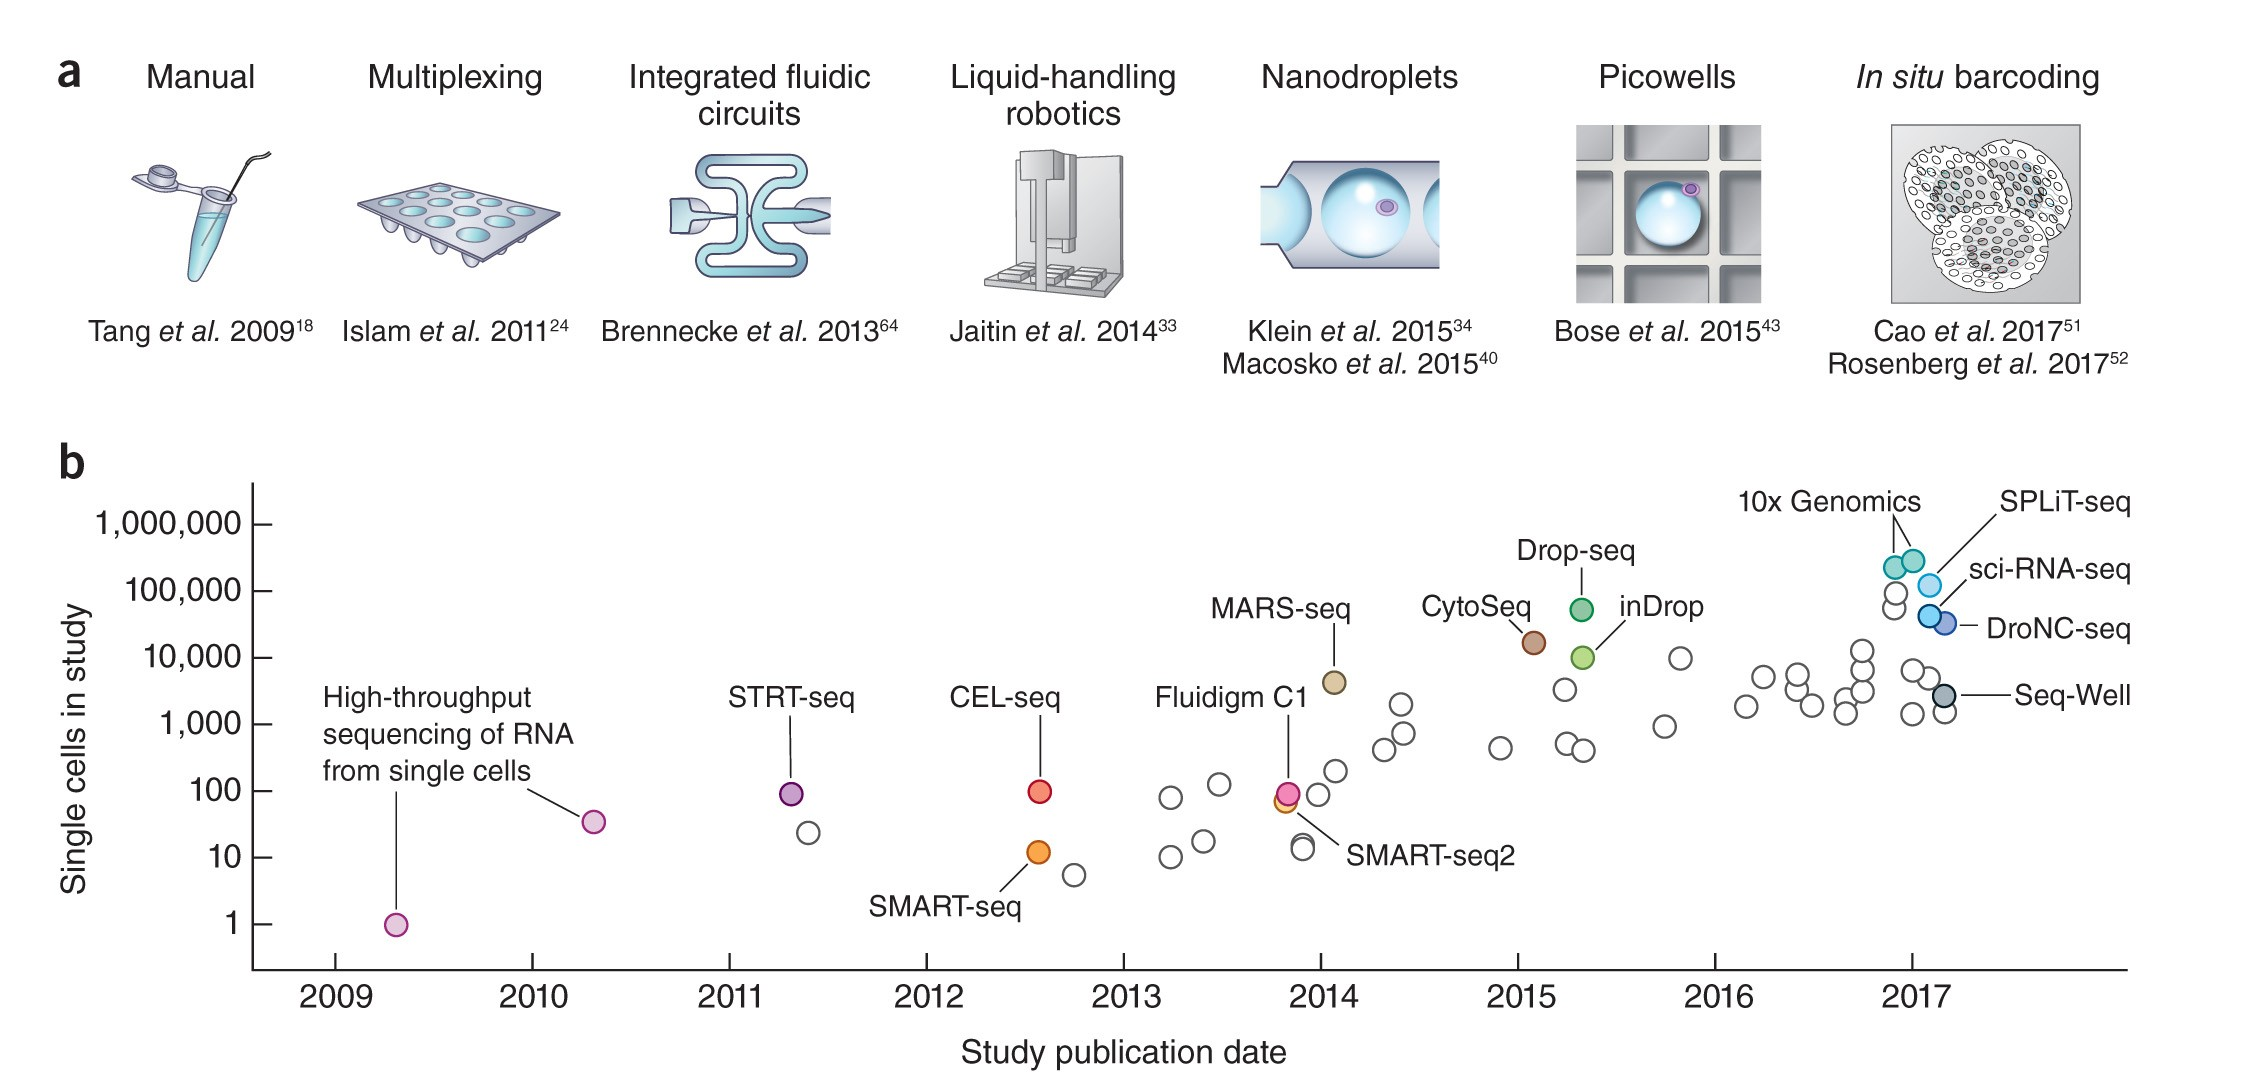
\includegraphics[width=15cm]{Chapter1/Fig/scrnaseq_technologies_svensson2018.jpg}
% \caption[\textbf{scRNA-seq technologies}]{\textbf{Scale of scRNA-seq experiments}.\\
% Technologies that have allowed....

% % make own version adding SmartSeq3 etc 

% adapted from \cite{svensson2018exponential}}
% \label{fig:scrnaseq_technologies}
% \end{figure}

% \subsubsection{Plate-based technologies}

% SmartSeq2

% \subsubsection{Droplet-based technologies}

% DropSeq, 10X Genomics

% \subsubsection{other technologies}

% multi omics aproaches (\cite{stuart2019integrative})

% spatial transcriptomics

% perturb seq

% %\subsection{Analysis of scRNA-seq data}

% \subsection{Computational modelling of scRNA-seq}

% Analysis of scRNA-seq data requires a new set of considerations, largely concerning technical signals, that were not relevant for bulk RNA-sequencing work. 
% Moreover, the resolution of this single-cell data also allows a number of more powerful analysis techniques to be applied.
% This section describes, in brief, how a typical single-cell RNA-sequencing dataset may be analysed.

% \cite{stegle2015computational}

% \subsubsection{Low-level analysis}

% reads QC 

% alignment

% mapping QC

% \subsubsection{Normalisation and batch correction}

% Count matrix
% 10 Genomics: UMI counts
% Smasrtseq2: expected counts or TPM (similar to bulk)

% cell QC (e.g. remove cells with less than xx total counts, yy total genes)
% possibly deal with doublets etc - in our case, donor assignment is also here

% normalisation (account for differences due to read coverage etc)

% log transformation (variance stabilising)

% \textbf{feature selection} (isolate most informative genes, e.g. highly variable genes - HVGs)\\

% genes that behave differently from your expected mean-variance relationship

% optional: centering+scaling - standardising

% batch correction (stronger than normalisation) 
% mutual nearest neighbours (MNN, \cite{haghverdi2018batch}) - and then fastMNN
% canonical correlation analysis (CCA, implemented in Seurat \cite{butler2018integrating}), Stuart et al 2019
% LIGER iNMF (negative matrix factorisation),
% Harmony (\cite{nowotschin2019emergent}) - iterative soft k means (fastest)
% Welch et al 2019, Korsunsky et al 2019


% \subsubsection{Computational analysis}

% \textbf{dimensionality reduction}

% \gls{pca} was first introduced by Pearson over a hundreds years ago (\cite{}, see section 1), yet remains one of the most widely used tools \\

% \textbf{clustering}

% unsupervised\\

% \textbf{pseudotime}

% PCA, diffusion maps\\

% \textbf{DE}

% DESeq, edgeR



% \subsubsection{Visualisation techniques}

% Even after application of a dimension-reduction procedure, a typical dataset will retain more than three biologically important dimensions in its new subspace, which makes visual representation of the data challenging. 

% Transforming high-dimensional data into a human-readable format is therefore an important challenge for single-cell data interpretation.

% scRNA-seq data visualisation techniques used in this thesis: 



% \begin{itemize}
%     \item \gls{pca}
%     \item t-distributed stochastic neighbour embedding (tSNE) \cite{maaten2008visualizing}
%     \item uniform manifold approximation and projection (UMAP) \cite{mcinnes2018umap}
% \end{itemize}


% Workflow packages:

% \begin{itemize}
%     \item scanpy
%     \item scater / scran / Single cell experiment (SCE)
%     \item seurat
%     \item SINCERA
% \end{itemize}




% \subsection{General applications of scRNA-seq in biology}

% Studies of single-cell transcriptomes allow us to directly investigate properties of individual cells, i.e. mRNA abundance. 
% Thus gene regulation is analyzed at the single cell level and, unlike traditional bulk RNA- sequencing, cell-to-cell heterogeneity can be considered.

% By measuring gene expression in development, differentiation, or other responses, we can start to understand cellular phenotypes as well as the regulatory processes that determine these phenotypes. 
% In many experiments cells are sampled at many time points and gene expression is assessed.

 
% \subsubsection{Atlases}

% Human Cell Atlas (HCA)

% The human cell atlas aims to provide a comprehensive reference map of all human cells
% \cite{rozenblatt2017human}
% \subsubsection{Cancer}
% \subsubsection{Immunology}
% \subsubsection{Development}

% developmental trajectories 
% A particular advantage of single-cell methods is the ability to capture cells at various developmental
% stages in a single experiment.

% \subsubsection{lineage tracing}

% \newpage

\subsection{The `resolution revolution'}
\label{sec:scrnaseq}

The first single-cell RNA sequencing (scRNA-seq) experiment was published in 2009, and it involved profiling of only eight cells \cite{tang2009mrna}. 
Seven years later, 10X Genomics released a dataset of 
% more than 
1.3 million cells \cite{102016our}.
All in all, in the last decade, over 1,000 scRNA-seq datasets have been published 
\cite{svensson2018exponential, svensson2019curated, svensson2020single},
using a number of different technologies 
\cite{islam2011characterization, hashimshony2012cel, ramskold2012full, picelli2013smart, sasagawa2013quartz, jaitin2014massively, macosko2015highly,klein2015droplet, gierahn2017seq, zheng2017massively, hagemann2020single}
(\textbf{Fig. \ref{fig:scrnaseq_technologies}}). \\

\begin{figure}[h]
\centering
% 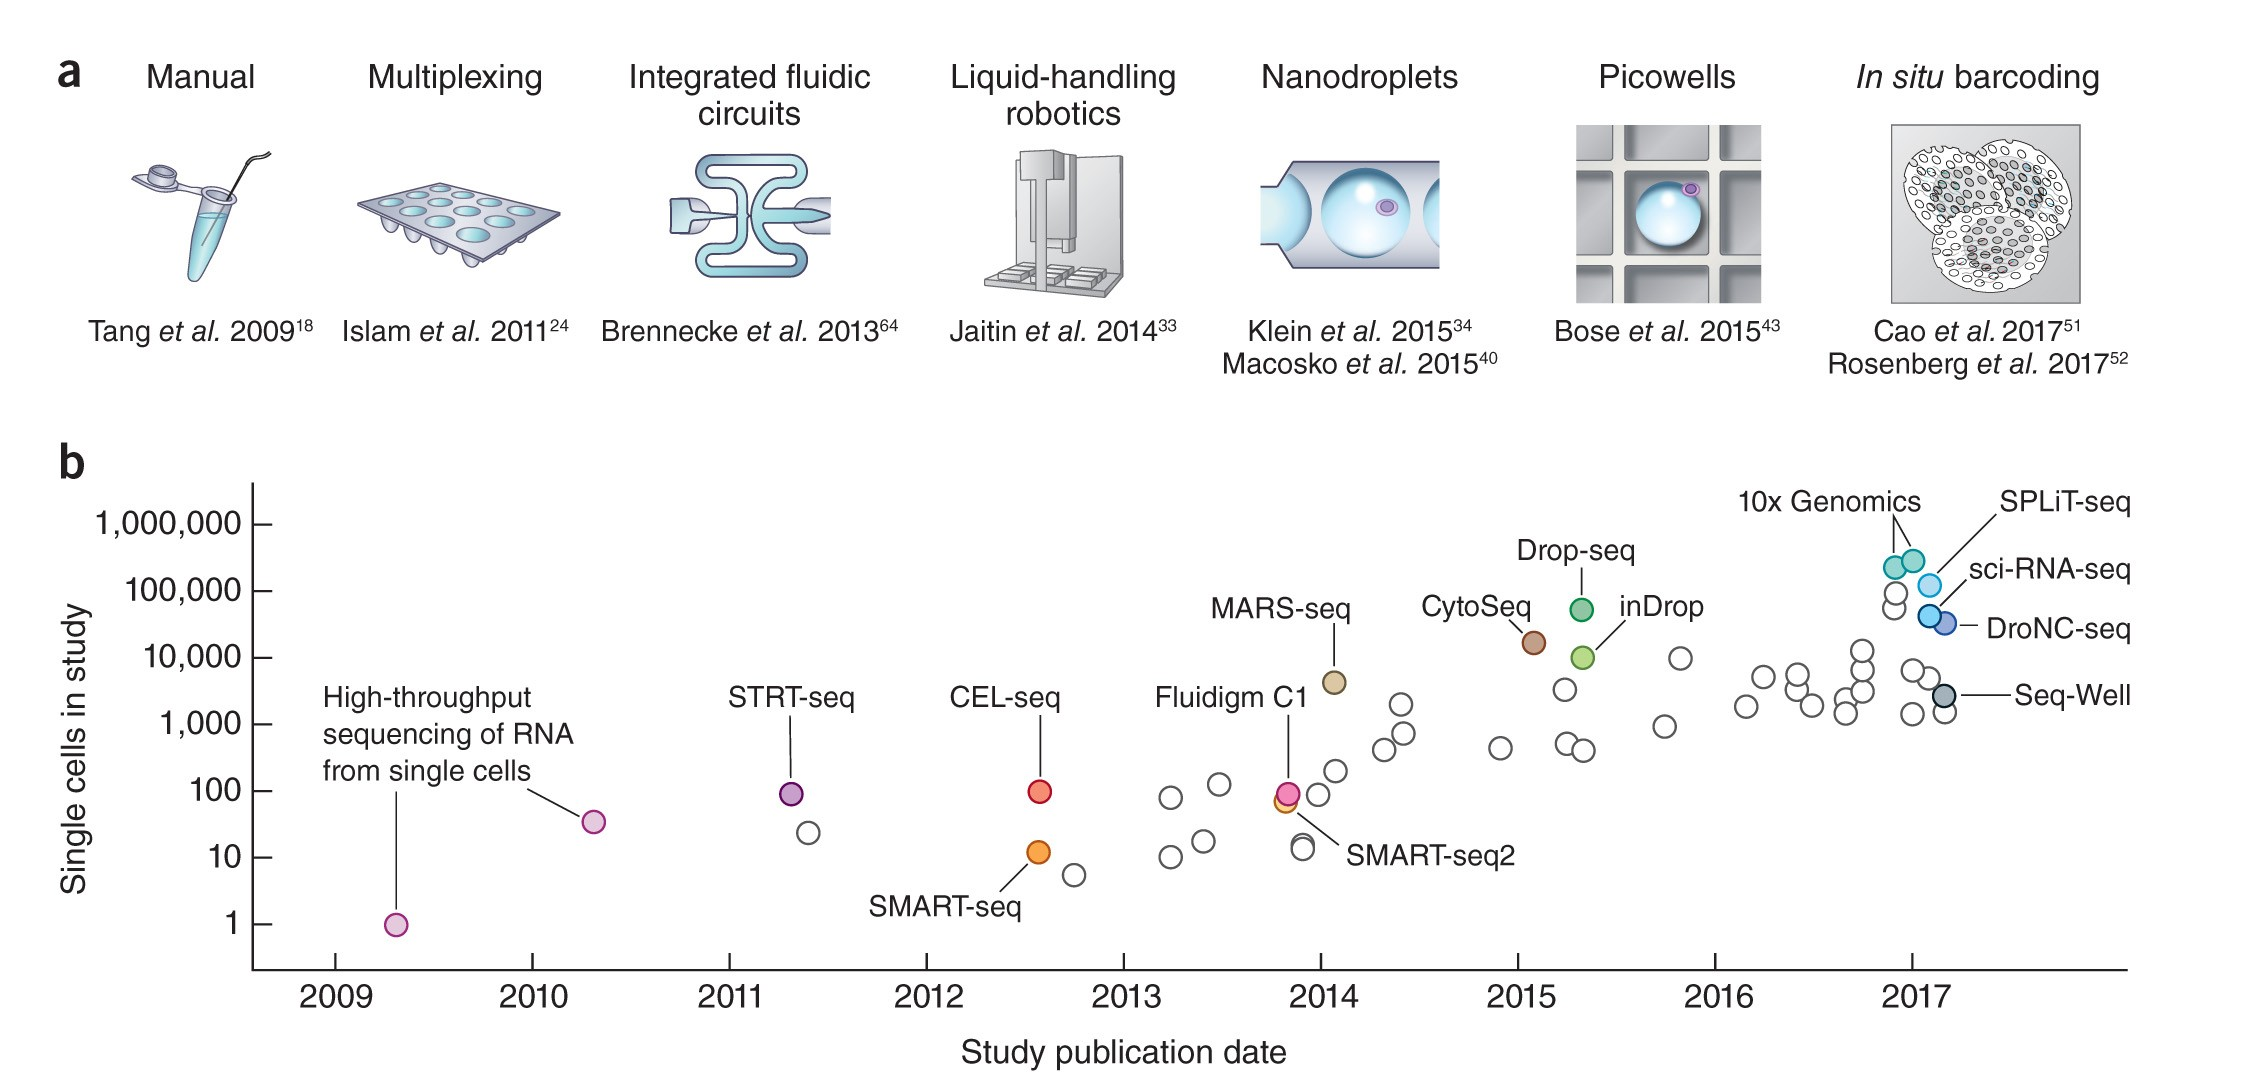
\includegraphics[width=15.5cm]{Chapter1/Fig/scrnaseq_technologies_svensson2018.jpg}
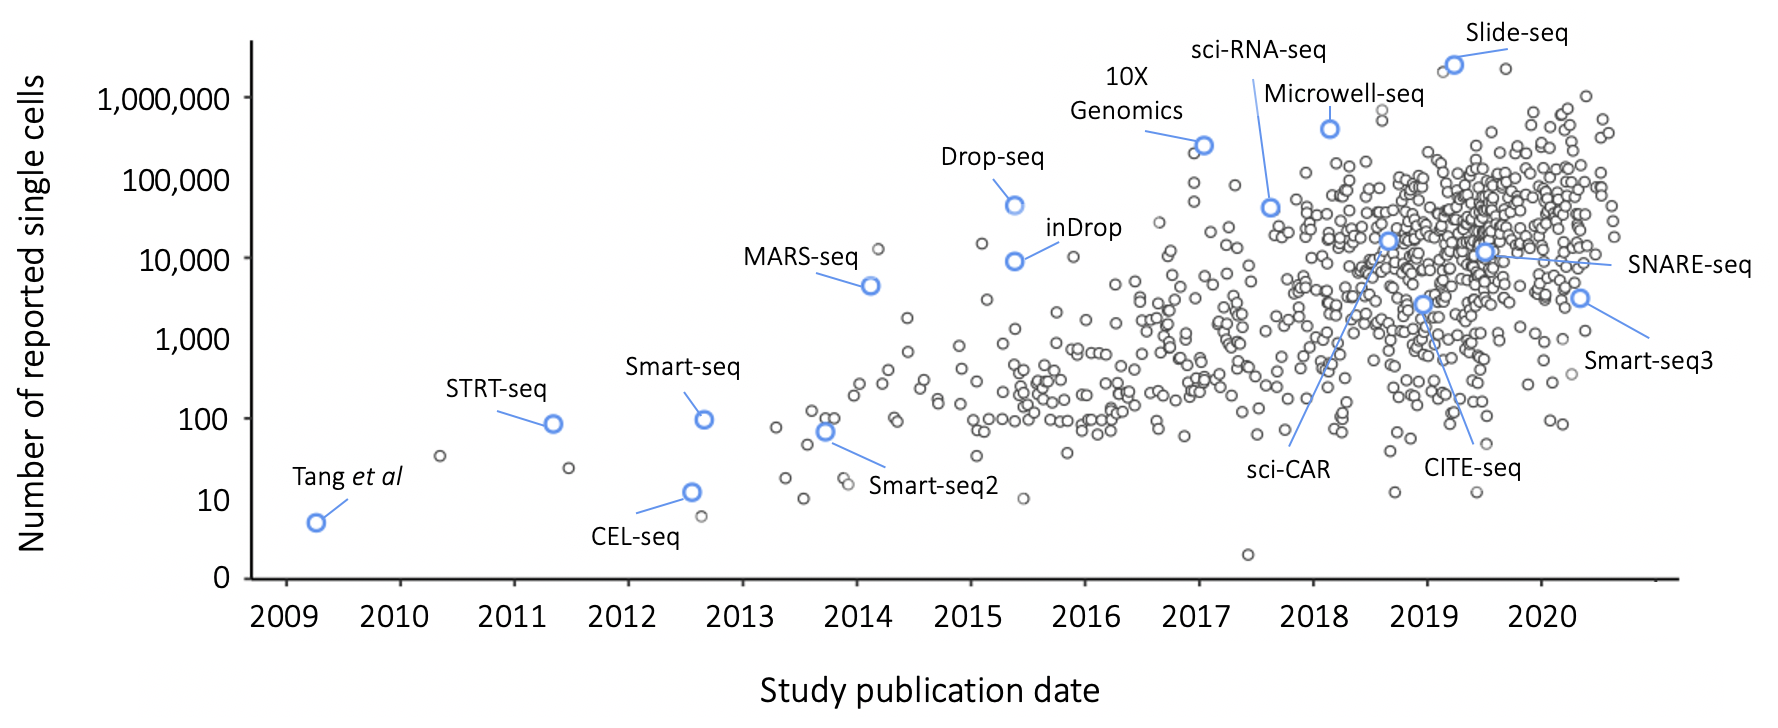
\includegraphics[width=16cm]{Chapter3/Fig/scrnaseq_ncells.png}
\caption[scRNA-seq technologies]{\textbf{Scale of scRNA-seq experiments}.\\
Number of single cells reported in all scRNA-seq publications to date (as collected in \cite{svensson2020single}, y axis), ordered by publication date (x axis).
Key scRNA-seq methods are indicated.
Similar to \cite{svensson2018exponential}.}
\label{fig:scrnaseq_technologies}
\end{figure}

% These methods can be categorised in different ways, but two of the most important aspects are quantification (full-length vs tag-based) and capture (microwell- or plate-, microfluidic-, droplet-based).
% In particular, SmartSeq2 vs 10x used here.
% plate-based: more genes
% droplet-based: more cells\\ 
Single cell RNA-seq protocols differ extensively in terms of scalability, costs and sensitivity 
% % [221, 128] 
\cite{ziegenhain2017comparative, svensson2018exponential}.
However, they can be broadly categorised into methods that are 
% % There are two broad sets of methods for applying single-cell RNA-seq—
`plate-based' or `droplet-based', based on the capture technology used
(\textbf{Fig. \ref{fig:scrnaseq_plate_vs_droplet}}).\\

% From Jonny's thesis
% Initially, most studies used plate-based assays (e.g. SmartSeq), where library preparation is performed manually on cells sorted into and lysed in individual wells of a microwell plate.
% (Figure 1.1) [17, 18].
% Robotic and microfluidic systems (e.g., Fluidigm C1) have been developed to automate some of these processes.
Initially, most studies used plate-based assays, where cells are isolated using micropipettes or flow cytometry into individual wells of a plate, where the library preparation is performed (\textbf{Fig. \ref{fig:scrnaseq_plate_vs_droplet}}).
This class of methods include single-cell tagged reverse transcription sequencing (STRT-seq \cite{islam2011characterization}), Cell Expression by Linear amplification and Sequencing (CEL-seq \cite{hashimshony2012cel}), massively parallel single cell RNA-seq (MARS-seq \cite{jaitin2014massively}) and Smart-seq \cite{ramskold2012full, picelli2013smart, hagemann2020single}. 
\\

% merge below (Jonny + Ricard)
On the other hand, droplet-based methods employ microfluidics to capture individual cells in nanolitre-sized droplets, each loaded with all the necessary reagents for library preparation.
% reagents and unique labels: reverse transcription and transcript labelling take place within these small volumes.
% (Figure 1.1). 
The droplet suspension is later broken down for pooling of cell libraries prior to sequencing (\textbf{Fig. \ref{fig:scrnaseq_plate_vs_droplet}}). 
% Droplet-based methods are based on the use of droplet microfluidics technology [246]. 
% merge below
These methods have been developed by academic groups (InDrop \cite{klein2015droplet} and Drop-seq \cite{macosko2015highly}) and commercially, by 10X Genomics (Chromium \cite{zheng2017massively}). 
These protocols share similar technologies, particularly the use of \glspl{umi} to correct for biases in PCR amplifications \cite{kivioja2012counting}. 
% Differences lie in the barcode design, cDNA amplification step and bead manufacturing [246].
\\

Each approach has its own advantages and disadvantages.
The main advantage of plate-based methods is the higher quality of libraries and, in the case of Smart-seq, the full length transcript information which enables the quantification of splice variants \cite{westoby2018simulation}, allele-specific expression \cite{jiang2017scale} and RNA velocity information \cite{la2018rna}. 
However, this comes at the expense of lower cellular throughput, processing hundreds or thousands of cells compared to the hundreds of thousands that droplet-based methods can achieve.
Indeed, by capturing cells in individual droplets, 
% summarise this
each containing all necessary reagents for library preparation, 
droplet-based protocols allow the profiling of thousands or even millions of cells in a single experiment. 
This, however, comes at the cost of reduced sensitivity.
Additionally, current droplet methods capture gene information exclusively from the 3’ or 5’ end of each transcript, and are more likely to produce `doublets', where two different cells become labelled with the same barcode (\textbf{Fig. \ref{fig:scrnaseq_plate_vs_droplet}}). 
% In contrast, the main drawback lies on the low throughput.
% Yet, multiplexing techniques and the addition of molecular barcodes to cDNA fragments allow the parallel processing of multiple experiments, thereby increasing the scale of each experiment.
% As a trade-off, the increased high throughput of droplet-based approaches 
% [252, 238, 222] (Figure 1.1).
% Each approach has its own advantages and disadvantages.
% Plate-based methods tend to provide higher-quality libraries at the cost of lower cellular throughput, processing hundreds or thousands of cells compared to the hundreds of thousands that droplet methods can achieve.
% summarise below
% More subtle differences also differentiate the two sets of methods. 
% To capture rare cell types with known cell-surface markers, it is generally more efficient to flow-sort and prepare plates of single-cell libraries rather than the brute-force approach of capturing more cells outright using a droplet method. 
% Additionally, current droplet methods capture gene information exclusively from the 3’ or 5’ end of each transcript, while some plate approaches generate reads from across entire transcripts; the latter allows splice-variant and allele-specific transcriptional information to be retrieved. 
% Finally, droplet methods are more likely to produce `multiplet' cell transcriptomes, where multiple different cells become labelled with the same barcode. 
% This is largely due to the lack of user oversight (e.g., it is more difficult to identify attached pairs of cells) and the possible reuse of cell barcodes from the labelling beads. 
% The doublet rate in droplet experiments is proportional to the number of loaded cells [21]; hence a user may reduce the rate of this confounding, albeit by sacrificing cost-efficiency, by loading fewer cells per sample.
\\

\begin{figure}[h]
\centering
% 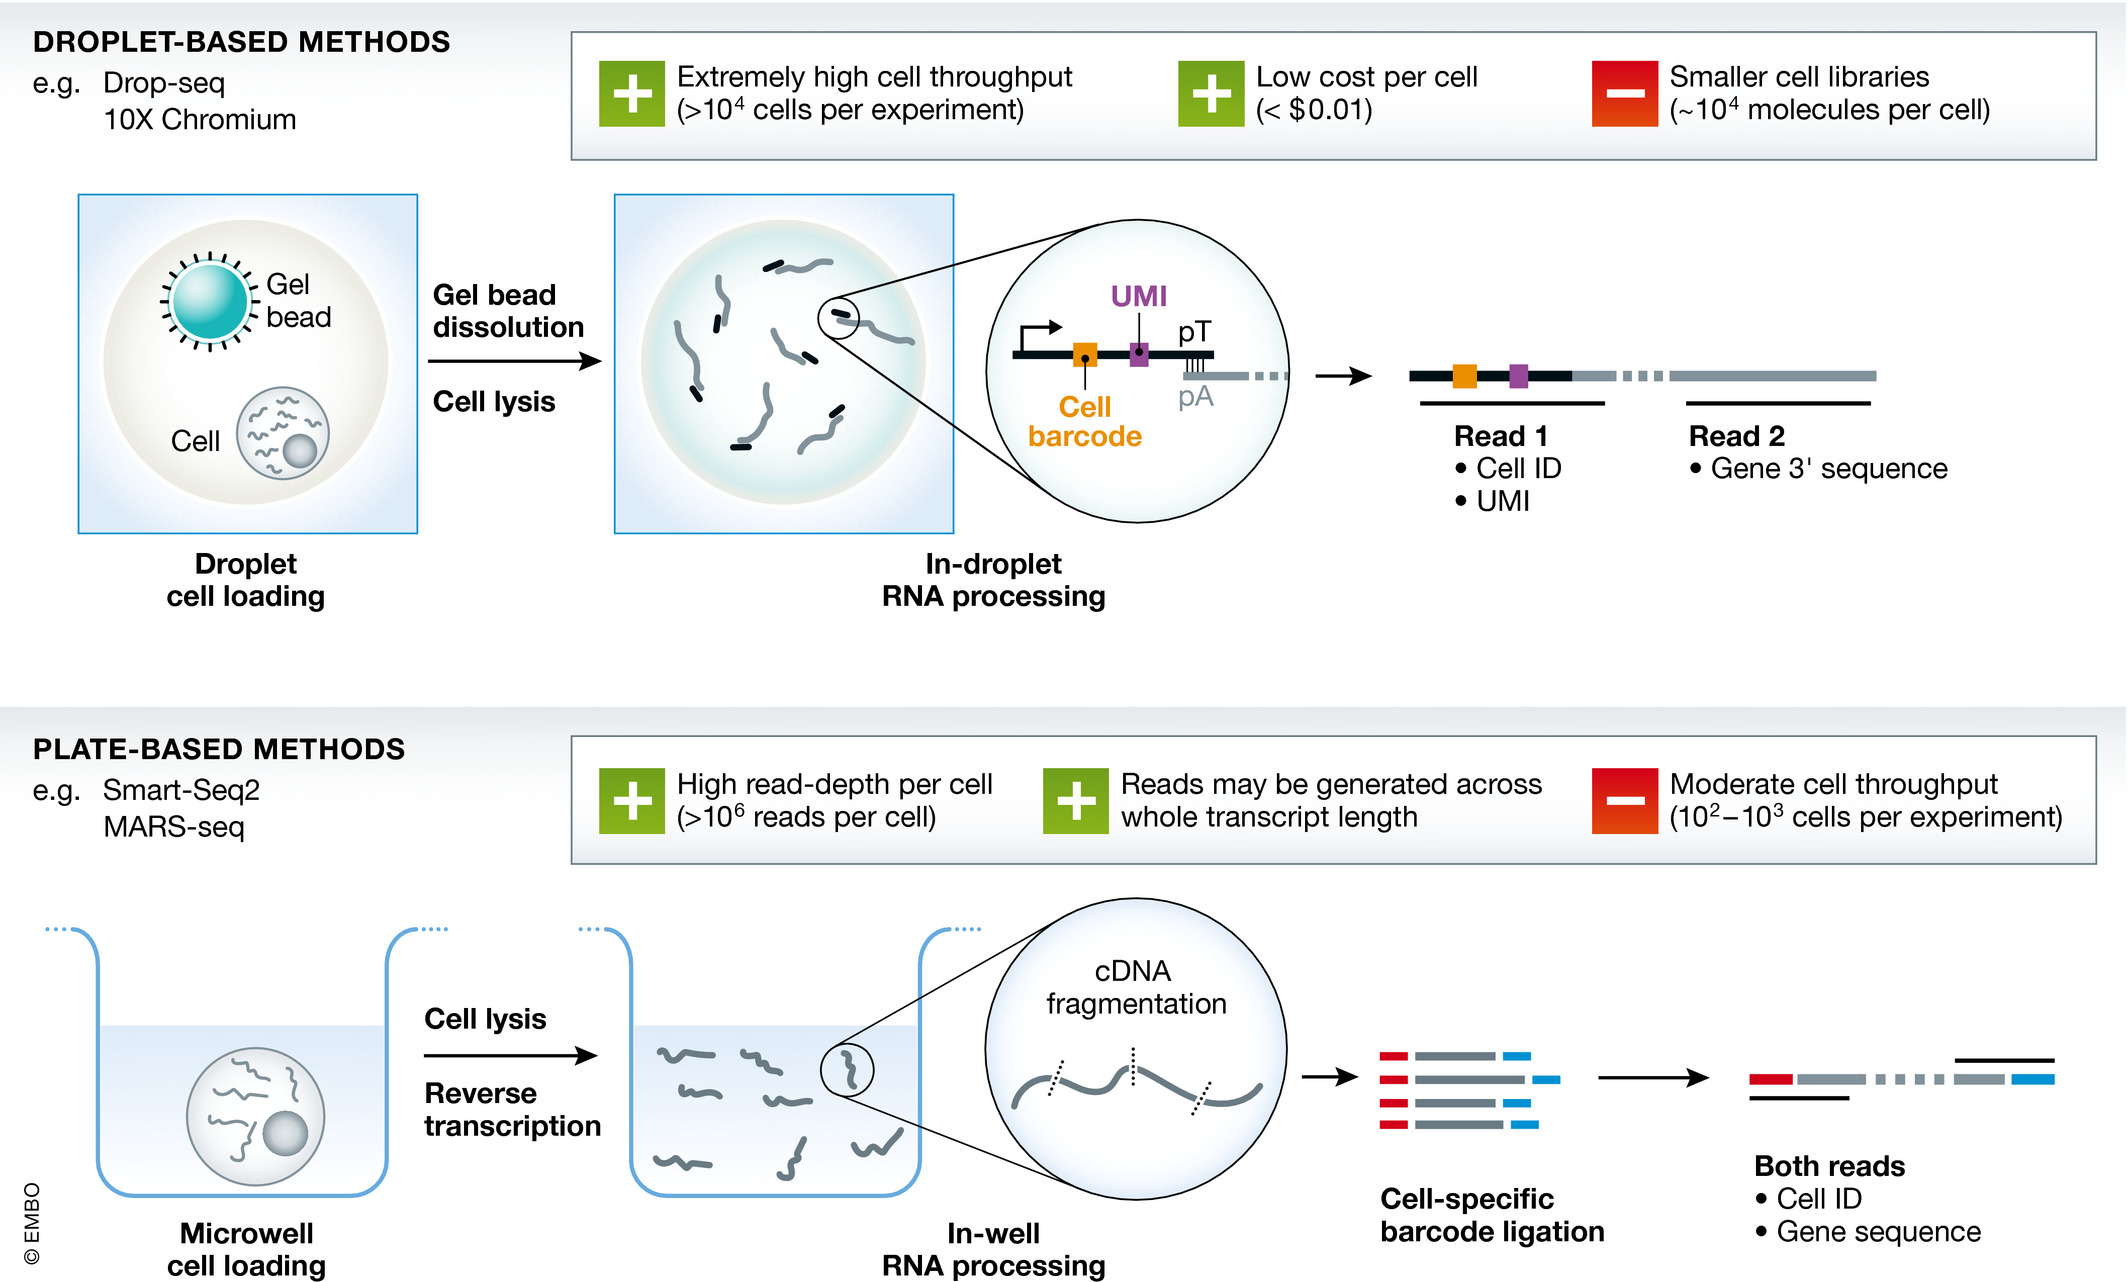
\includegraphics[width=14.5cm]{Chapter3/Fig/plate_vs_droplet_griffiths2018.jpg}
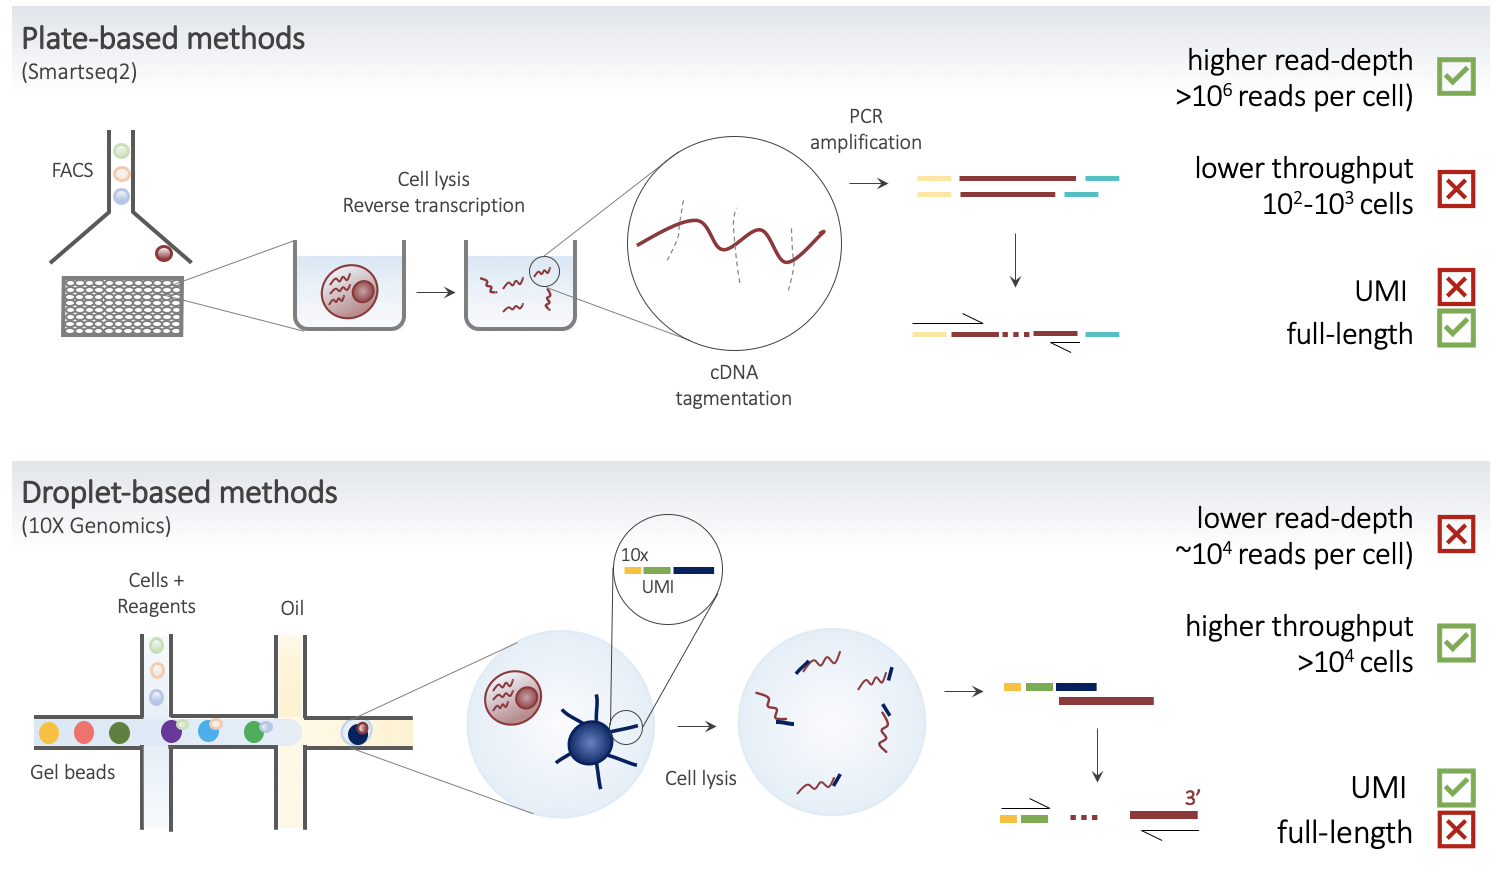
\includegraphics[width=16cm]{Chapter3/Fig/plate_vs_droplet.png}
\caption[scRNA-seq plate vs droplet]{\textbf{Plate-based vs droplet-based methods for scRNA-seq}.\\
An illustration of the key differences between plate-based methods (exemplified by SmartSeq2 \cite{picelli2013smart}) and droplet-based methods (represented by 10X Genomics Chromium \cite{zheng2017massively}).
The key trade-off is between the cell-throughput (much higher for droplet-based methods) and the read-depth per cell (higher for plate-based methods).
Additionally, the full-length transcripts obtained using SmartSeq2 allow quantification of allele-specific expression and splice variants, which are not possible with 3' tag 10X data.
Finally, all droplet-based methods include UMI, which allow the robust quantification of PCR duplicates.

Note that these last two differences (in terms of UMIs and full length) specifically hold true for the two methods shown here (and used in this thesis: SmartSeq2 and 10X Genomics).
Indeed, not all plate-based methods provide full-length transcript information (e.g. MARS-seq \cite{jaitin2014massively} and CEL-seq \cite{hashimshony2012cel} do not).
In contrast, the most recent SmartSeq3 \cite{hagemann2020single} can include UMIs, despite being a plate-based method.
Figure similar to \cite{griffiths2018using}.}
\label{fig:scrnaseq_plate_vs_droplet}
\end{figure}

% \newpage

% Analysis of scRNA-seq data requires a new set of considerations, largely concerning technical signals, that were not relevant for bulk RNA-sequencing work.
% Moreover, the resolution of this single-cell data also allows a number of more powerful analysis techniques to be applied.
% This section describes, in brief, how a typical single-cell RNA-sequencing dataset may be analysed.
In the last 10 years, technological improvement (\textbf{Fig. \ref{fig:scrnaseq_technologies}}) has gone hand-in-hand with computational advances to analyse the resulting data, which require a new set of considerations that were not relevant for bulk RNA-seq data.
% maybe highlight that droplet-based method are more and more popular
% Today, scRNA-seq is an established technique
Indeed, to complement the explosion of scRNA-seq studies published, an entire ecosystem of computational methods for analysing them has emerged.
% \\ 
% (add figure/table?) 
In some cases, those methods have been directly borrowed from bulk RNA-sequencing methods; other times, methods tailored specifically for single cell data were proposed \cite{stegle2015computational, zappia2018exploring, luecken2019current}.
% \\

\clearpage

Single cell-specific bioinformatics workflows such as Cell Ranger \cite{zheng2017massively}, indrops \cite{klein2015droplet}, SEQC  \cite{azizi2018single}, or zUMIs \cite{parekh2018zumis}
have been developed to perform 
% the very first 
raw data processing tasks,
% by
% pipelines such as 
% for example 
% .
% Namely, these 
i.e. read-level QC, assignment of reads to their cell barcodes and mRNA molecules of origin (i.e. `demultiplexing'), alignment to the reference genome, and quantification. 
Additional methods allow the assignment of cells to their donor of origin, in case of  multi-individual pooled designs \cite{kang2018multiplexed, mccarthy2020cardelino}.
% Generating single‐cell data from a biological sample requires multiple steps. Typical workflows incorporate single‐cell dissociation, single‐cell isolation, library construction, and sequencing
% After the alignment of the sequencing reads to a reference genome, 
The data resulting from a scRNA-seq experiment are typically represented as an integer matrix of gene expression levels, with entries representing the number of sequenced reads (or molecules, if UMIs were used) assigned to a particular gene in a specific cell \cite{griffiths2018using}.
Starting from these count matrices, a common scRNA-seq analysis workflow may be divided into pre-processing steps and downstream analysis \cite{luecken2019current} - and scRNA-seq-specific tools have been implemented for several of the steps along the pipeline.\\

In particular, methods have been proposed to perform  cell calling, i.e. to detect, and exclude, empty droplets \cite{lun2019emptydrops}, doublets \cite{wolock2019scrublet, mcginnis2019doubletfinder, depasquale2018doubletdecon}, and ambient RNA \cite{young2020soupx}.
% Next, standard cell QC steps involve ..
% The distributions of these QC covariates are examined for outlier peaks that are filtered out by thresholding
% cell QC (number of reads, genes, MT, most expressed)
Moreover, methods for normalisation have been described in \cite{lun2016pooling, vallejos2017normalizing, weinreb2018spring}.
% CPM
% Thus, when gene expression is compared between cells based on count data, any difference may have arisen solely due to sampling effects. Normalisation addresses this issue by e.g. scaling count data to obtain correct relative gene expression abundances between cells.
% normalisation, size factors (UMI?)
% Add normalisation.
After normalisation, data matrices are typically log(x+1)‐transformed. 
Additionally, several novel methods allow to correct for confounding factors including batch effects \cite{haghverdi2018batch, butler2018integrating, nowotschin2019emergent, stuart2019comprehensive, welch2019single, polanski2020bbknn} and
cell cycle effects \cite{scialdone2015computational, mcdavid2016reply}.
To ease the computational burden on downstream analysis tools, reduce the noise in the data, and to visualise the data, one can use several approaches to reduce the dimensionality of the dataset.
First, feature selection, for example by detecting highly variable genes (HVGs) \cite{brennecke2013accounting, yip2019evaluation}.
Next, dimensionality reduction is performed either using linear methods, such as \gls{pca}, or non-linear methods, with the latter being preferred for visualisation purposes.
In particular, t-distributed stochastic neighbour embedding (tSNE)  \cite{maaten2008visualizing} and uniform manifold approximation and projection (UMAP) \cite{mcinnes2018umap} are extremely popular (for a review of other methods, see \cite{moon2018manifold}). 
Downstream analysis methods can be classified into cell-level and gene-level.
The former include clustering \cite{kiselev2017sc3, traag2019louvain}, often followed by cell type annotation \cite{kiselev2018scmap}, as well as pseudotime inference \cite{haghverdi2016diffusion, trapnell2014dynamics, bendall2014single, wolf2019paga}.
Finally, single cell-specific methods have been developed for gene-level analyses, including differential expression analysis \cite{finak16others}, and gene regulatory networks identification \cite{matsumoto2017scode, chan2017gene, aibar2017scenic}.\\


% such as read alignment, cell calling and visualisation \cite{maaten2008visualizing, mcinnes2018umap} as well as to perform higher level tasks such as batch correction \cite{haghverdi2018batch, butler2018integrating, nowotschin2019emergent, stuart2019comprehensive, welch2019single, polanski2020bbknn}, clustering \cite{kiselev2017sc3, traag2019louvain} and pseudotime inference \cite{haghverdi2016diffusion}.\\

A typical workflow for single cell RNA-seq data implemented in R can be found on Bioconductor\footnote{at \url{https://bioconductor.org/packages/devel/bioc/vignettes/scran/inst/doc/scran.html} and

\url{https://osca.bioconductor.org}} using scRNA-seq specific R packages scran \cite{lun2016step, risso2016scrnaseq}, scater \cite{mccarthy2017scater}, and SingleCellExperiment 
\cite{lun2019singlecellexperiment}.
Other pipelines for scRNAseq data analysis include 
Seurat \cite{butler2018integrating},
Scanpy \cite{wolf2018scanpy}, 
and SINCERA \cite{guo2015sincera}. 
% \\


% \begin{figure}[htbp]
% \centering
% 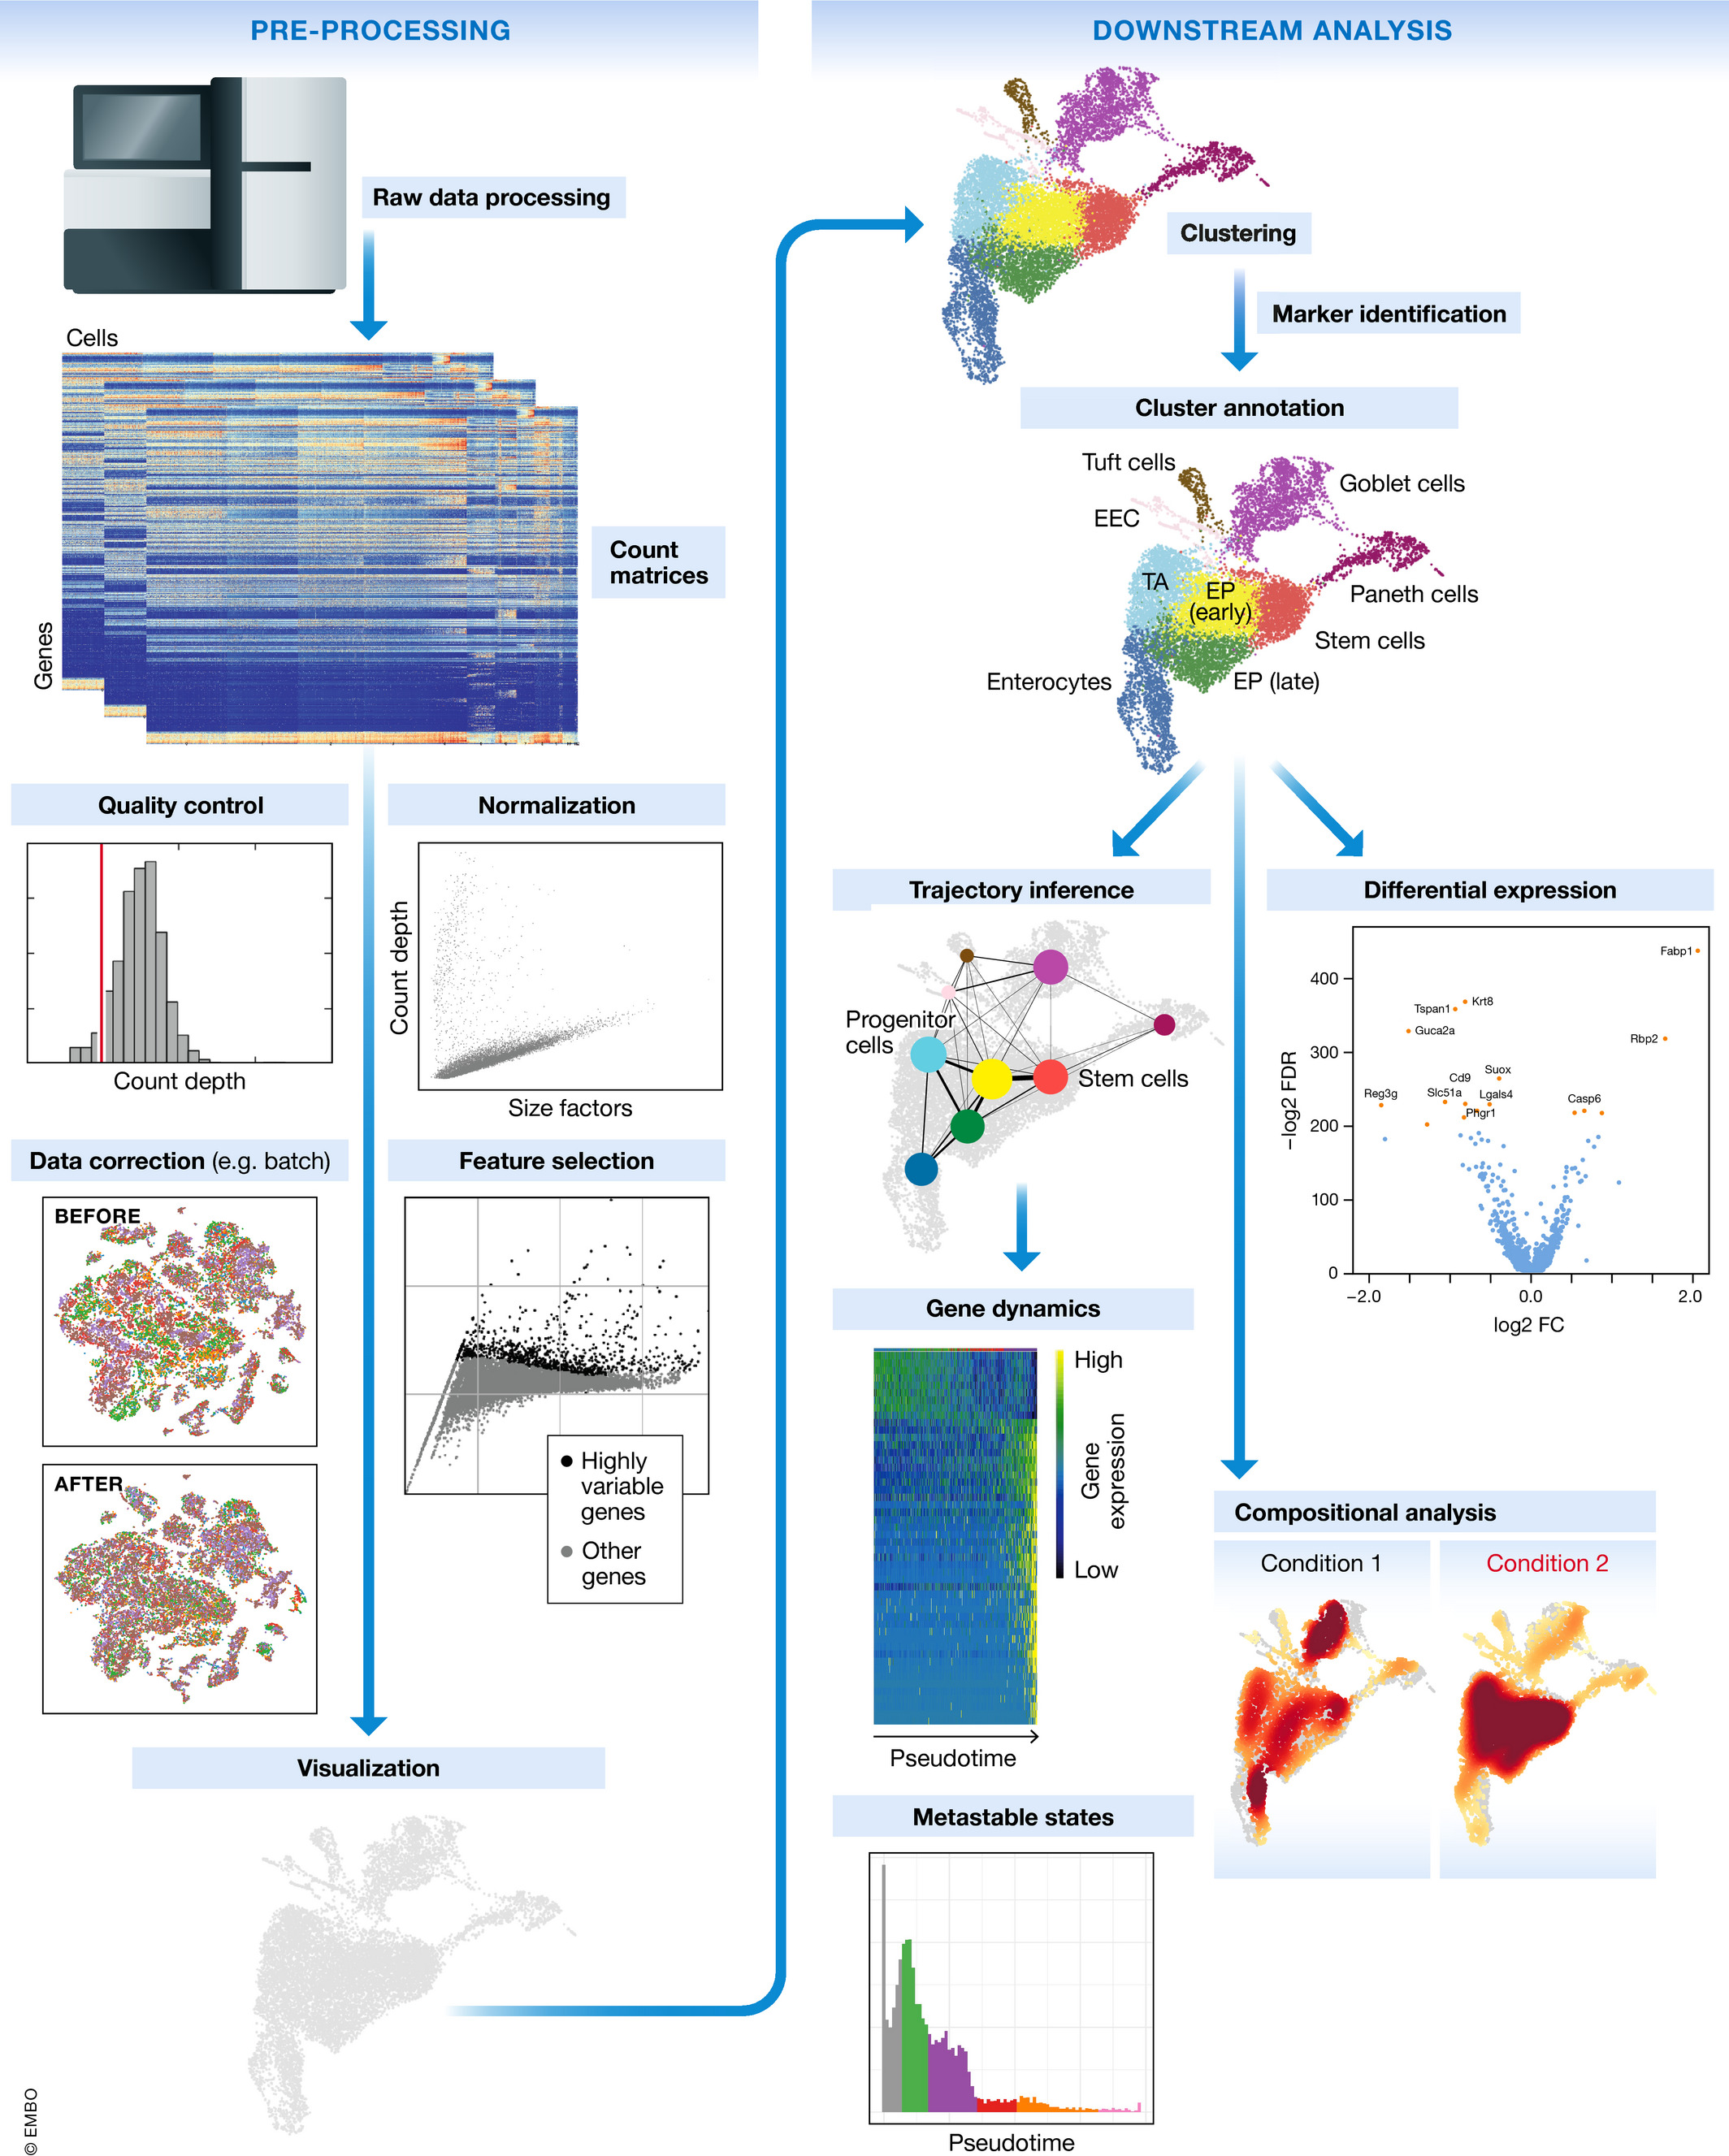
\includegraphics[width=14.5cm]{Chapter3/Fig/scrnaseq_analysis_luecken2019.jpg}
% \caption[scRNA-seq analysis pipeline]{\textbf{scRNA-seq analysis pipeline}.\\
% % (make own version)
% Adapted from \cite{luecken2019current}}
% \label{fig:scrnaseq_analysis_pipeline}
% \end{figure}

% Here I will only mention a few key steps.



% \subsubsection{Low-level analysis}
% reads QC 
% alignment
% mapping QC

% cell QC (e.g. remove cells with less than xx total counts, yy total genes)
% possibly deal with doublets etc - in our case, donor assignment is also here
% normalisation (account for differences due to read coverage etc)
% log transformation (variance stabilising)

% feature selection (isolate most informative genes, e.g. highly variable genes - HVGs)
% genes that behave differently from your expected mean-variance relationship



% Several platforms implement the entire processing workflow, or at least large portions of it.
% These include R packages seurat \cite{stuart2019comprehensive} and SINCERA (SINgle CEll RNA-seq profiling Analysis, \cite{guo2015sincera}) and python package scanpy \cite{wolf2018scanpy}. 



% \subsection{Computational modelling of scRNA-seq}

% Analysis of scRNA-seq data requires a new set of considerations, largely concerning technical signals, that were not relevant for bulk RNA-sequencing work. 
% Moreover, the resolution of this single-cell data also allows a number of more powerful analysis techniques to be applied.
% This section describes, in brief, how a typical single-cell RNA-sequencing dataset may be analysed.



% \subsubsection{Normalisation and batch correction}

% Count matrix
% 10 Genomics: UMI counts
% Smartseq2: expected counts or TPM (similar to bulk)



% \textbf{feature selection} (isolate most informative genes, e.g. highly variable genes - HVGs)\\

% genes that behave differently from your expected mean-variance relationship

% optional: centering+scaling - standardising

% batch correction (stronger than normalisation) 
% mutual nearest neighbours (MNN, \cite{haghverdi2018batch}) - and then fastMNN
% canonical correlation analysis (CCA, implemented in Seurat \cite{butler2018integrating}), Stuart et al 2019
% LIGER iNMF (negative matrix factorisation),
% Harmony (\cite{nowotschin2019emergent}) - iterative soft k means (fastest)
% Welch et al 2019, Korsunsky et al 2019


% \subsubsection{Computational analysis}

% \textbf{dimensionality reduction}

% \gls{pca} was first introduced by Pearson over a hundreds years ago (\cite{}, see section 1), yet remains one of the most widely used tools \\

% \textbf{clustering}

% unsupervised\\

% \textbf{pseudotime}

% PCA, diffusion maps\\

% \textbf{DE}

% DESeq, edgeR



% \subsubsection{Visualisation techniques}

% Even after application of a dimension-reduction procedure, a typical dataset will retain more than three biologically important dimensions in its new subspace, which makes visual representation of the data challenging. 

% Transforming high-dimensional data into a human-readable format is therefore an important challenge for single-cell data interpretation.

% scRNA-seq data visualisation techniques used in this thesis: 



% \begin{itemize}
%     \item \gls{pca}
%     \item t-distributed stochastic neighbour embedding (tSNE) \cite{maaten2008visualizing}
%     \item uniform manifold approximation and projection (UMAP) \cite{mcinnes2018umap}
% \end{itemize}

\newpage

\subsection{Single cell eQTL mapping}
\label{sec:sc_eqtl}

With the ability to identify cell types and states in an unbiased manner \cite{kolodziejczyk2015technology, trapnell2015defining}, the use of 
% population-scale 
scRNA-seq data, combined with genotype information, is uniquely positioned to provide an extra layer 
of information on the regulatory role of common genetic variants
% (including disease-associated variants) 
on
% to our understanding of the genetic regulation of 
gene expression, across a plethora of cell types and states.
As a consequence, single cell \gls{eqtl} mapping 
% has emerged as a field, 
is increasingly feasible,
% as the cost of sequencing reduces,
and promises to improve our understanding of genetic regulation both in health and disease across tissues \cite{wills2013single, van2018single, sarkar2019discovery, jerber2020population, van2020single1, cuomo2020single}.
\\

When performing \gls{eqtl} mapping using scRNA-seq profiles, a first important step is to verify the feasibility of traditional `mean level' \gls{eqtl} mapping, i.e. to reproduce \glspl{eqtl} previously identified using bulk RNA-seq.
Only then can we explore new avenues and alternative types of \gls{eqtl} analyses, which are especially enabled by the single cell resolution (\textbf{Fig. \ref{fig:sc_eqtl}}).\\

\begin{figure}[h]
\centering
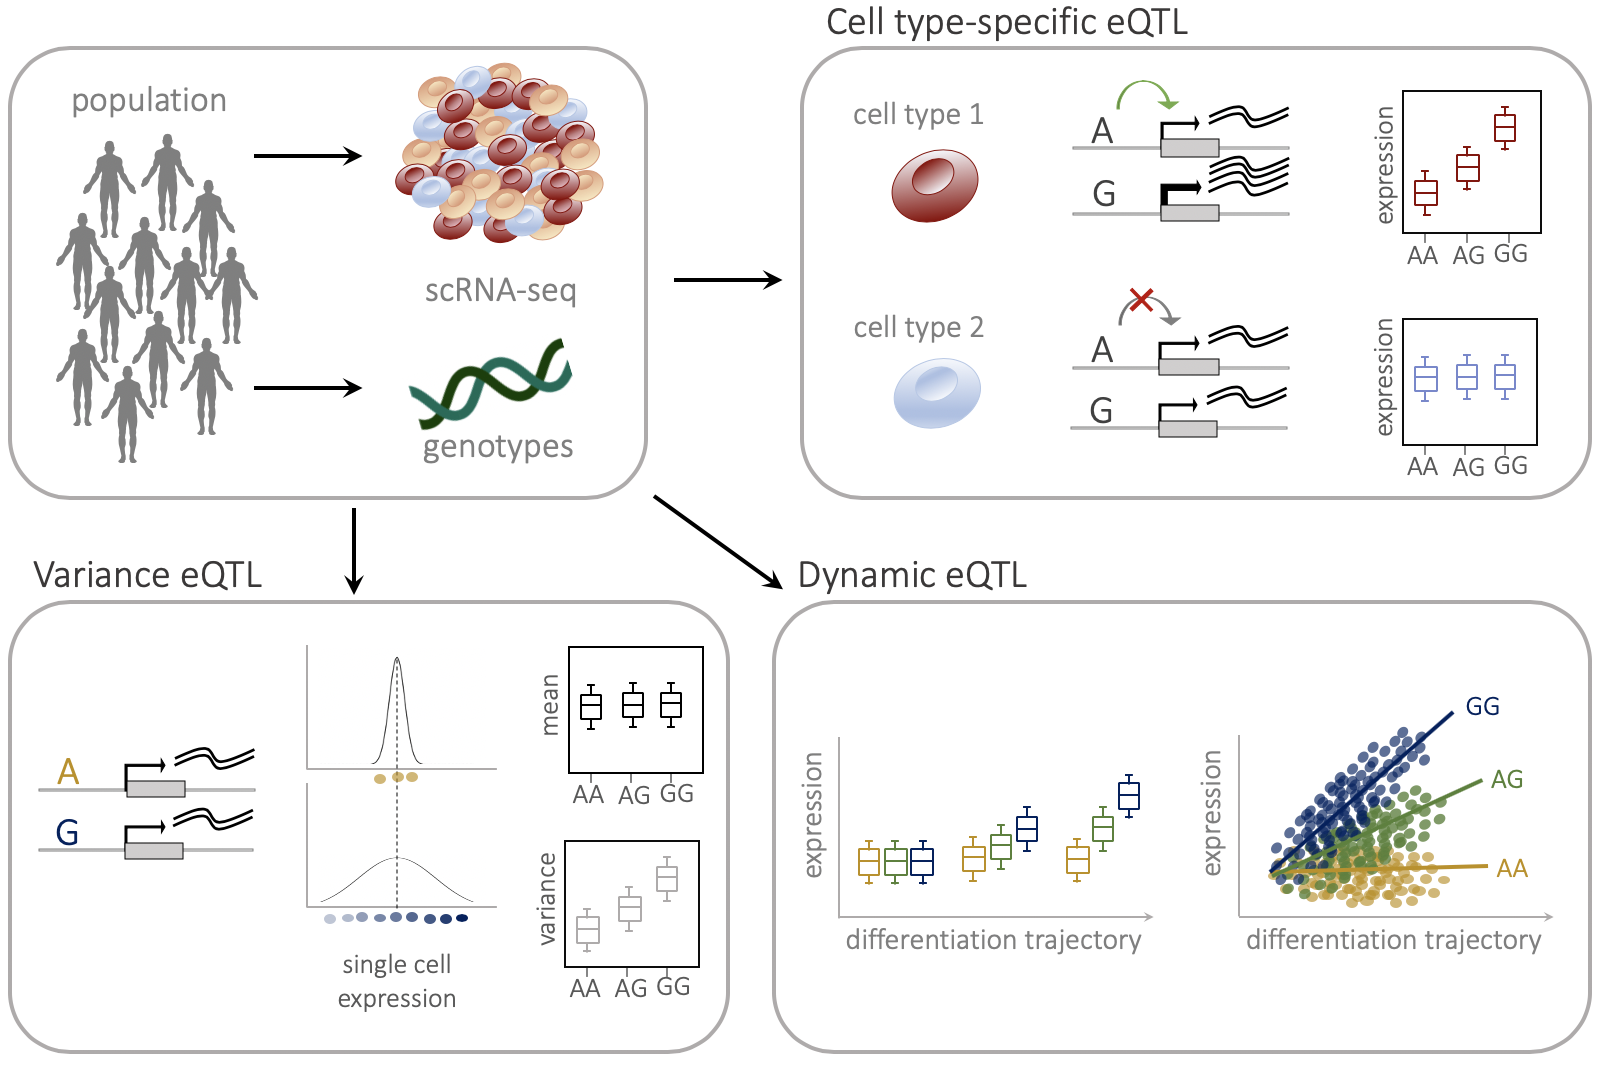
\includegraphics[width=14cm]{Chapter3/Fig/sc_eqtl.png}
\caption[Single cell eQTL]{\textbf{Overview of single cell eQTL mapping methods}.\\
Matched genotypes and scRNA-seq data from several individuals allow the detection of cell type-specific \gls{eqtl}, variance \gls{eqtl} (genetic effects on cell-to-cell transcriptional variability), and dynamic \gls{eqtl} (dynamic genetic effects along cellular differentiation or other cellular states).}
\label{fig:sc_eqtl}
\end{figure}

In this chapter, we address the first point (i.e. mapping mean-level sc-\gls{eqtl}).
To do so, we leverage bulk and single cell gene expression of matched human 
% \gls{ipsc}
iPSC
lines from around 100 donors to identify general guidelines for \gls{eqtl} mapping using scRNA-seq data.
% We compare several manners of normalising and aggregating expression across cells per donor as well as different models to test for \gls{eqtl} and compare to equivalent results obtained when using bulk RNA seq data.
% Whilst for most individuals we have plate-based sc-RNAseq data (SmartSeq2, \cite{picelli2013smart}), we also have data using the 10X Genomics platform \cite{zheng2017massively} for a subset of around 30 samples, which allows us - to an extent - to also compare results across single cell technologies.

\newpage

\section{What is different in single cell data?}
% \section{What can we learn from single cell data?}

When we perform \gls{eqtl} mapping, we are interested in finding differences in expression level between individuals, when stratified by their genotypes at a genomic locus of interest (\textbf{page 
\pageref{fig:eqtl}}). 
Under the assumption that we are looking at an otherwise homogeneous population of cells (e.g. all cells are from the same cell type), it is reasonable to consider the total (or the average) expression for each individual and gene, across all cells.
When we use bulk RNA sequencing expression profiles, that is essentially what happens: all cells from an individual are pooled, the mRNA is extracted, reverse-transcribed to cDNA, and then sequenced. 
The resulting reads are then mapped onto a reference genome, and the expression level of each gene is quantified as the number of reads (raw counts) obtained from one donor that uniquely map to that gene, after normalisation, e.g. transcripts per million (TPM)\footnote{i.e. for every 1,000,000 RNA molecules in the RNA-seq sample, x came from this gene/transcript.}. 
A bulk RNA-seq experiment, therefore, results in one individual measure of `abundance' of each gene for each donor. 
Such a measure results in 
% measure is the results of 
aggregating over 
hundreds of thousands of cells
% XX-YY cells (ZZ on average, \cite{})
and, at least for expressed genes (e.g. average TPM > 1), the vector of gene expression across individuals follows a distribution that can be approximated as Gaussian \cite{piras2015reduction}.
% \\
% The intuition here is that 
% Pool of RNA transcripts from many genes (low probability for a given gene), get a sample to sequence. 
% Poisson: sampling from large n, small p (samples are technical replicates)
% (biological replicates - NB > Poisson, larger variance )
% As discussed,
% % in section 1.3 of the Introduction, 
% robust experimental methods are now available to assay expression profiles of individual cells, using scRNA-seq.
% , allowing to assay the genome-wide transcriptome of hundreds to thousands of individual cells. 
On the other hand,
whilst scRNA-seq data provides increased resolution and promises great insights into cellular function, the data are also much sparser, and the number of cells that can be assayed for an individual is limited compared to bulk (often as little as 10-100 cells). 
In addition, the number of cells that can be assessed often varies substantially from individual to individual.
As a result, the distribution of total counts from a single cell experiment as opposed to its corresponding bulk experiment has lower mean (fewer cells, fewer reads, \textbf{Fig. \ref{fig:sc_bulk_counts}}) and higher variance (due to the variable number of cells across donors, \textbf{Fig. \ref{fig:sc_bulk_counts}} vs \textbf{Fig. \ref{suppl_fig:counts_sc_ncells}}).
% (on average XX compared to YY for bulk RNA-seq, \cite{}).
% Moreover, in addition to observing a smaller number of cells (and therefore total reads) for an individual as compared to bulk, the read distribution typically does not follow a normal distribution, mostly due to very different amounts of reads coming from different donors. \\

\begin{figure}[h]
\centering
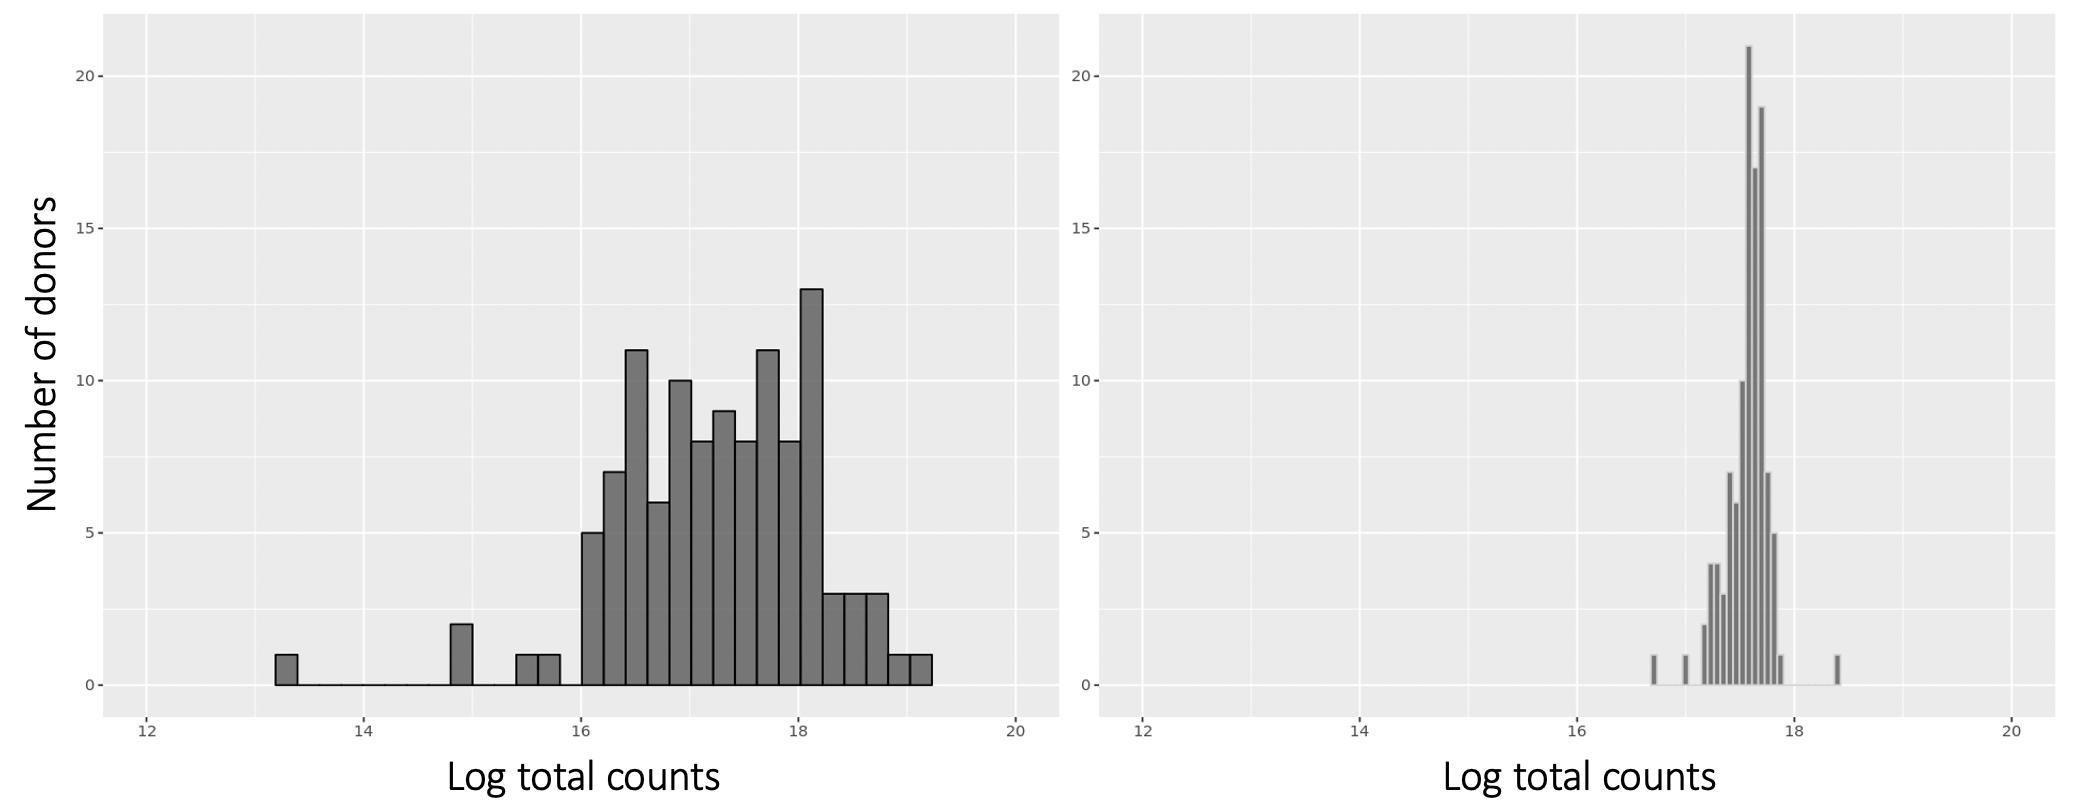
\includegraphics[width=13cm]{Chapter3/Fig/count_distribution_sc_vs_bulk.png}
\caption[Distribution of reads]{\textbf{Distribution of reads}.\\
Distribution of total reads (across all genes) per individual for matched 
% \gls{ipsc}
iPSC
data (108 individuals) using single cell (left, from \cite{cuomo2020single}) and bulk (right, from \cite{mirauta2018population}) RNA-seq data.}
\label{fig:sc_bulk_counts}
\end{figure}
% This is in part due to the `double sampling' that is inherent of the technology: there is a chance of not sampling any reads from one gene in one cell, and there is a chance of not sequencing any reads from that cell at all.

% Add differences in number of total reads, read distribution, describe “double sampling” process.

\newpage

% \section{Data}
\section{Single cell and bulk RNA-seq profiling of iPSCs}

The data I use in this chapter to benchmark methods for single cell \gls{eqtl} mapping 
% were generated by colleagues at the Sanger Institute
% % \footnote{The Ludovic Vallier lab, at the Wellcome Trust Sanger Institute, Cambridge, UK.
% % Full acknowledgments and contributions for this project can be found in the next chapter, at page \pageref{contr:chapter4}.}
% , using human \gls{ipsc} lines from the
% HipSci
% % \gls{hipsci} 
% resource (see section 
% % \ref{sec:ips_genetics}).
% 1.2.6). 
% They 
were generated as part of a larger study, where \gls{ipsc} lines from over 100 donors (from HipSci) are differentiated towards definitive endoderm.
A pooled design was adopted, where cells from 4-6 lines were differentiated together, to avoid for individual genetic differences to be confounded with batch variation. 
Cells were later assigned to their donor of origin using Cardelino \cite{mccarthy2020cardelino}. 
Next, cells were collected at four time points (day0, day1, day2, day3) and sequenced using Smartseq2 \cite{picelli2013smart}, a plate-based single cell technology (\textbf{Fig. \ref{fig:scrnaseq_plate_vs_droplet}}).
This study was published earlier this year \cite{cuomo2020single}, and I discuss the key results from it in the next chapter (\textbf{Chapter 
\ref{chapter4}}).
% 4}).
\\

% In this chapter, 
Here,
I focus on the earliest time point (i.e. day0), where cells are still pluripotent, prior to cell differentiation.
We expect iPS cells to be fairly homogeneous, so it is the ideal cell type to use to perform this kind of study.
After QC\footnote{Some QC steps were performed for all time points jointly, therefore I refer the reader to the detailed QC pipeline described in the next chapter, at \textbf{page \pageref{fig:endodiff_qc_workflow}}.}, data was available from 9,661 iPS cells and 11,231 genes, from 112 unique unrelated donors, across 24 differentiation pools (\textbf{Fig. \ref{fig:ipsc_data}}). 
To map eQTL, I considered only donors with at least 10 cells, which excluded one donor, bringing the sample size down to 111.
The number of cells per individual varied widely, ranging from 10 to 383 iPS cells from individual to individual.
% OS: clarify that this is a homogenous cell population, hence comparison bulk <-> scRNA. You should also add somehwere that the dat aare pooled and demulitplexed ? The terminoloyg “pool” is not explained anywhere. Generally, I’d expect a bit more datil. HOw mnany cells per person? What is the effective read depth per person in the bseudo bulk? HOw was pseudo bulk calculated, etc. 
% \\
% Add QC steps here? Maybe briefly and then refer to chapter 4.
% Also more on HipSci lines (used): sex, age, ethnicity
% \subsection{Comparison partners}
% \begin{itemize}
%     \item bulk RNA-seq with matched samples (i.e. individuals for which we have both bulk and sc-RNAseq data, n=109/112)
%     \item bulk RNA-seq all samples (i.e. all samples for which we have bulk RNA-seq data, n=462)
%     \item matched 10x scRNA-seq (for a subset of common samples, n=29/112)
% \end{itemize}
% \newpage
Additionally, we have matched deep bulk RNA-sequencing profiles generated as part of the HipSci project \cite{kilpinen2017common} for the vast majority of cell lines used (108/111, 97\%). 
% , as well as for a large number of other HipSci lines (676 human \gls{ipsc} lines from 462 unique donors in total).
Finally, we have scRNA-seq data measured using a droplet-based technology (10X Genomics \cite{zheng2017massively}) for a subset of common lines (29 \gls{ipsc} lines, from five of the experimental pools, \textbf{Fig. \ref{fig:ipsc_data}}). 

\begin{figure}[h]
\centering
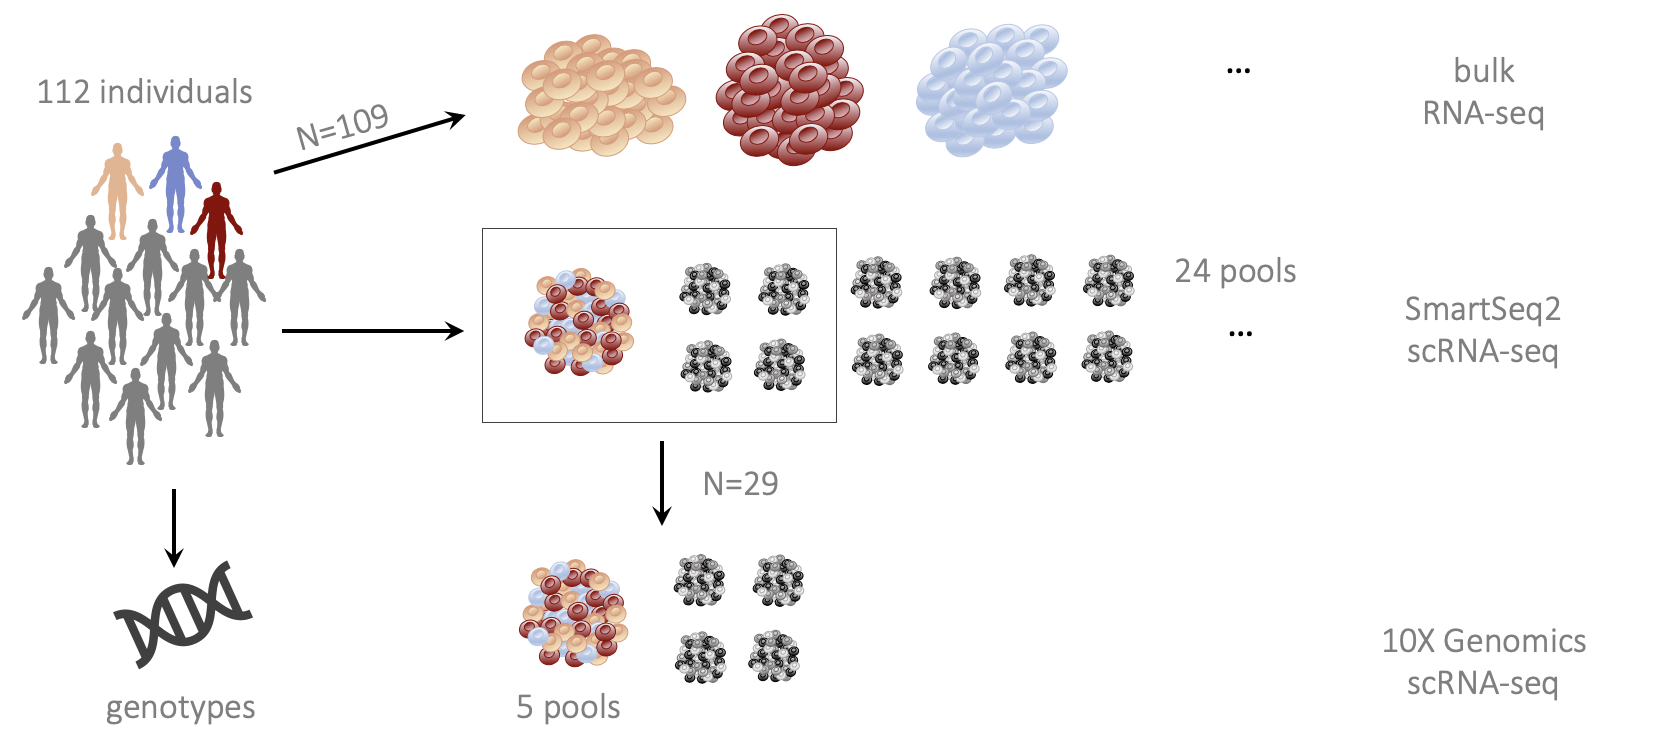
\includegraphics[width=14cm]{Chapter3/Fig/ips_data.png}
\caption[iPSC data]{\textbf{Overview of iPSC data used in this chapter}.\\
We use SmartSeq2 \cite{purcell2007plink} data from 111 \gls{ipsc} lines (from 111 individuals) from \cite{cuomo2020single}, across 24 experimental pools, each containing cells from 4-6 lines (middle).
For 108 of those lines, we have bulk RNA-seq profiles from \cite{mirauta2018population} (top).
Finally, for five of the pools (corresponding to 29 individuals/lines), we also have scRNA-seq data sequenced using the 10X Genomics pipeline \cite{zheng2017massively} (bottom).}
\label{fig:ipsc_data}
\end{figure}

\section{eQTL mapping pipeline}

To map \glspl{eqtl}, I use a pipeline primarily written by Marc Jan Bonder, to which Bogdan Mirauta, Daniel Seaton, Na Cai and myself have also contributed. 
It is a wrapper around LIMIX \cite{lippert2014limix, casale2015efficient}, and it is publicly available at \url{https://github.com/single-cell-genetics/limix_qtl}. \\

For all three eQTL maps (single cell SmartSeq2, bulk, single cell 10X), I used the same exact pipeline and tested the same set of genes (n=10,840).
In particular, I performed \textit{cis} \gls{eqtl} mapping, considering common (minor allele frequency > 5\%), in HWE (p value > 0.001)\footnote{HWE: Hardy-Weinberg equilibrium.}, variants within a \textit{cis}-region spanning 250 kb up- and down-stream of the gene body.
% for \textit{cis} QTL analysis. 
For each gene-SNP pair, the association test was performed using an LMM (\textbf{section
\ref{sec:linear_mixed_models}}):
% 2.3.2}):

\begin{equation}\label{eq:LMM_ipsc_eqtl}
    \mathbf{y} = \sum_i^{P}\alpha_i \mathbf{PC}_i + \mathbf{g}\beta + \mathbf{u} + \boldsymbol{\psi},  
\end{equation}
where 
\begin{itemize}
    \item $\mathbf{y}$ is the $N \times 1$ standardised\footnote{Centered at 0 and scaled to have variance = 1.} expression phenotype vector (details in next section),
    \item the first P=10 PCs calculated on the expression values (matrix with $\mathbf{y}$ as columns, before standardisation) are included as covariates\footnote{This is a common approach to correct for possible batch effects, which usually affect the expression of many genes, and therefore are detectable in the principal components of expression. 
    Moreover, these global effects are orthogonal to the effects of a single variant on the expression of one gene (see \textbf{section 
    % 2.2.4
    \ref{sec:confounders}}).}, and $\alpha_i$ are the corresponding weights,
    \item $\mathbf{g}$ is the $N \times 1$ vector of alleles for each sample at the locus tested (modelled as the number of minor alleles present - 0, 1 or 2), and $\beta$ is the corresponding effect size,
    \item $\mathbf{u}$ is a random effect term used to account for 
    the samples' 
    population structure, 
    % such that: 
    i.e.
    $\mathbf{u} \sim \mathcal{N}(\mathbf{0}, \sigma_g^2\mathbf{K})$, where $\mathbf{K}$ is an $N \times N$ kinship matrix estimated using PLINK \cite{purcell2007plink},
    \item and $\boldsymbol{\psi} \sim \mathcal{N}(\mathbf{0}, \sigma_n^2\mathbf{I})$, where $\mathbf{I}$ is the $N \times N$ identity matrix, is the noise vector.
\end{itemize}

\vspace{1.5mm}

\newpage

% Association tests were performed using a linear mixed model (LMM), accounting for population structure and sample repeat structure (see below) as random effects (using a kinship matrix estimated using PLINK\cite{purcell2007plink}).
% , with no observed confounding between population structure and experimental batch (Supplementary Fig. 24). 
All models were fitted using LIMIX \cite{lippert2014limix, casale2015efficient}. 
The significance was tested using a likelihood ratio test (i.e. $\beta \neq 0$, \textbf{section 
\ref{sec:hypothesis_testing}}).
% 2.2.1}).
In order to adjust for multiple testing (\textbf{section
\ref{sec:multiple_testing}}),
% 2.2.2}), 
we used a permutation scheme, analogous to the approach proposed in Ongen \textit{et al}. \cite{ongen2016fast}. 
Briefly, for each gene, we generated 1,000 permutations of the genotypes while keeping covariates, kinship, and expression values fixed. 
We then adjusted for multiple testing using this empirical null distribution.
To control for multiple testing across genes, we then applied the Storey procedure \cite{storey2003statistical}. 
Genes with significant \glspl{eqtl} were reported at FDR < 10\%.

% \newpage

\section{Single cell eQTL map of iPS cells}
\label{sec:sc_ipsc_eqtl}

Using the method just described, we first tested for associations between common genetic variants and gene expression in \glspl{ipsc} using our SmartSeq2 single cell data.\\

To reproduce bulk-like abundance measurements, we considered a gene's average expression level for each sample, across cells.
In particular, expression level is measured as log2(CPM+1)\footnote{CPM: counts per million, mapped reads are count-scaled by the total number of fragments sequenced per cell, times one million.} using scater \cite{mccarthy2017scater}.
% size factor?
\\

Since we did not use any batch correction method on the single cell expression data \textit{a priori}, we cannot exclude differences across batches.
As internal control we have, for a subset of donors (23/112), data from two (or three, in one case) distinct experimental batches.
We therefore compute average expression levels not for each individual line, but for each line-experiment combination (i.e. cell\_lineA-experiment1, cell\_lineA-experiment2), which enables effective correction for batch-to-batch differences using PCs as covariates (see above and \textbf{section
\ref{sec:confounders}}).
% 2.2.4}). 
% However, to be able to correct for possible batch differences, we considered two different average expression measures, when the same line was assessed in two different experimental batches - individual 1 in experiment A and individual 1 in experiment B are considered as two distinct samples.
% \subsection{Technical considerations}
The linear mixed model described in eq. \eqref{eq:LMM_ipsc_eqtl} can be readily adapted to include the resulting replicate measures from the same line: $N$ will now be not the number of unique lines but that of line-experiment combinations.
Additionally, both the genotype vector $\mathbf{g}$ and the kinship matrix $\mathbf{K}$ need to be adjusted\footnote{i.e. expanded, by duplicating genotype values across pool replicates.}, such that the latter is now in fact accounting at once for the population structure and the repeatedness of the samples tested (\textbf{Fig. \ref{fig:kinship_repeats}}). \\

Using this approach, I identified 1,833 genes with at least one \gls{eqtl} (from hereon `eGenes'), at FDR <10\%, out of 10,840 genes tested (17\%). 

\begin{figure}[h]
\centering
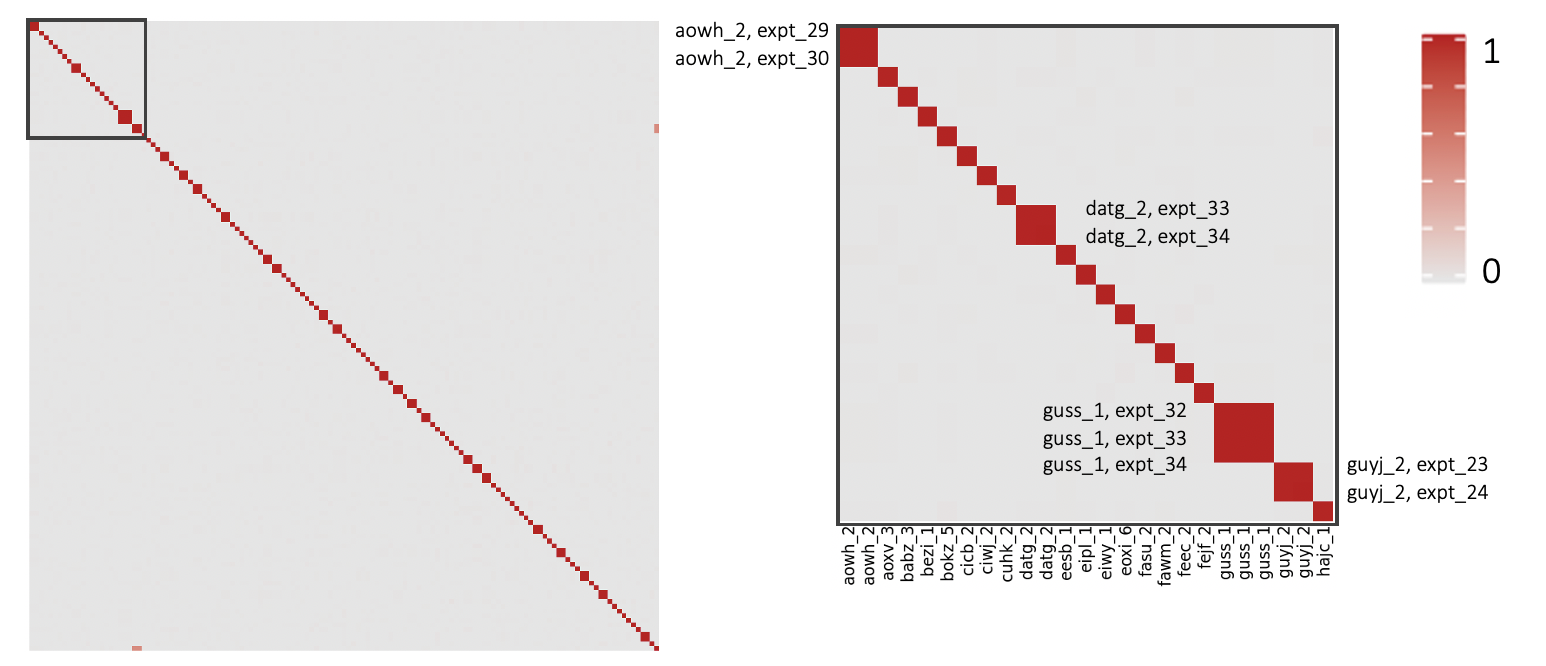
\includegraphics[width=14.5cm]{Chapter3/Fig/kinship_repeatedness.png}
\caption[Kinship for repeated samples]{\textbf{Kinship matrix highlighting repeated structure of samples used}.\\
Heatmap of the kinship matrix used to map \glspl{eqtl} using single cell data.
% Red indicated a maximum degree of relatedness, grey absence of it.
% The binary look of the heatmap suggests that lines used are from essentially unrelated individuals.
% The only pattern of relatedness is present for replicate observations from the same line, across experimental batches.
Replicate observations for a line across experimental batches are genetically identical, which is captured by the kinship (maximum relatedness, red).
Line-to-line relatedness is effectively 0 (grey), indicating unrelated individuals. 
On the right, zoom-in to only consider the first 20 \gls{ipsc} lines, highlighting the repeated samples.}
\label{fig:kinship_repeats}
\end{figure}

% \subsection{Results}

% CPM = readsMappedToGene * 1/totalNumReads * 10$^6$, totalNumReads - total number of mapped reads of a sample, readsMappedToGene - number of reads mapped to a selected gene




% \subsection{LMM}
% Association tests were performed using a linear mixed model (LMM), accounting for population structure and sample repeat structure (see below) as random effects (using a kinship matrix estimated using PLINK\cite{purcell2007plink}).
% % , with no observed confounding between population structure and experimental batch (Supplementary Fig. 24). 


\newpage

\section{Replication of iPSC eQTL using bulk RNA-seq}

For comparison, I performed \textit{cis}-\gls{eqtl} mapping using the matched bulk RNA-seq data.
% considering only the cell lines that had been used to map \gls{ipsc} \glspl{eqtl} from the scRNA-seq data (bulk data was available for 108 donors out of the 112 day0 single cell donors), 
I used the same pipeline (eq. \eqref{eq:LMM_ipsc_eqtl})\footnote{The only difference of course is that there were not multiple replicates from the same line in the bulk RNA-seq data, but the model in eq. \eqref{eq:LMM_ipsc_eqtl} still holds.} 
and tested the same set of genes. 
This yielded 2,908 significant genes at an FDR of 10\%
% (out of 10,736 genes tested, 27\%)
(27\% of genes tested). \\

I found that over 70\% of \glspl{eqtl} identified using scRNA-seq data were replicated in the bulk study, where a single-cell \gls{eqtl} lead variant (top variant per gene) was replicated if it achieved nominal significance (p value < 0.05) and had consistent direction of effect in the full set of results from the bulk \gls{eqtl} analysis (\textbf{Fig. \ref{fig:sc_bulk_egenes}}). \\

On the other hand, only around 50\% of the \gls{eqtl} identified (at FDR < 10\%) using bulk RNA-seq could be replicated
% \footnote{Defined as above: nominal significance (p value < 0.05) and same direction of effect.} 
in our single cell \gls{eqtl} map.
However, when we subsetted to \gls{eqtl} identified using bulk data at a more stringent FDR threshold (1\%), the replication proportion was much larger (76\%), and the more stringent the FDR threshold, the more bulk \gls{eqtl} we could replicate using single cell data (\textbf{Fig. \ref{fig:sc_bulk_egenes}}).
This result suggests that we are able to detect the stronger \gls{eqtl} signals, but lack the power (compared the corresponding test using bulk RNA-seq profiles) to identify smaller effects.
% \\

\begin{figure}[h]
\centering
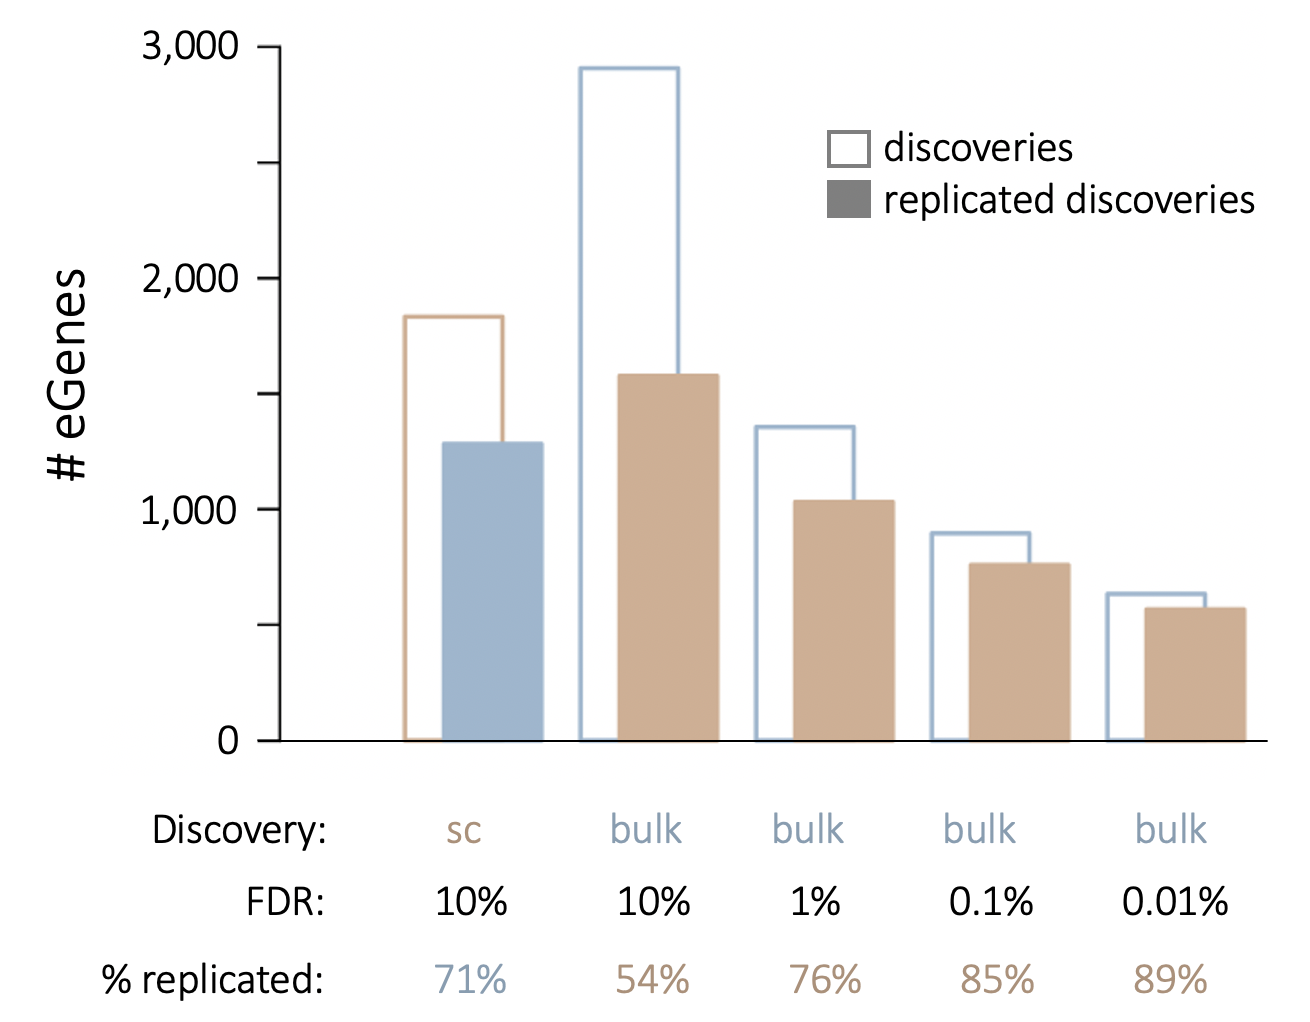
\includegraphics[width=12cm]{Chapter3/Fig/sc_vs_bulk_eqtl.png}
\caption[iPSC eQTL (bulk vs sc)]{\textbf{Replication of iPSC bulk eQTL using single cell data and vice versa}.\\
Replication of \gls{ipsc} \gls{eqtl} discovered with (matched-sample) bulk RNA-seq data using scRNA-seq data, and vice versa.
The total number of eGenes discovered is shown, along with the number of discoveries replicated in the other dataset, at various FDR thresholds. 
% Replication of bulk \gls{eqtl} in single-cell RNA-seq (SmartSeq2, here SS2) on same set of samples increases with significance ($\sim$55\% at FDR 10\%, $\sim$90\% at FDR 0.01\%, 4/112 samples were not present in the bulk RNA sequencing dataset).
sc: single cell.}
\label{fig:sc_bulk_egenes}
\end{figure}

% To compare the \gls{ipsc} \gls{eqtl} maps derived from bulk and single-cell RNA-seq data, we assessed the nominal significance (p value < 0.05) as well as the consistent direction of effect of single-cell \gls{ipsc} \gls{eqtl} lead variants (top variant per gene) in the full set of results from the bulk \gls{ipsc} \gls{eqtl} analysis and vice versa.

% To validate our approach, we also performed \gls{eqtl} mapping using deep bulk RNA-sequencing profiles from the same set of \gls{ipsc} lines (`iPSC bulk'; 10,736 genes tested) generated as part of the \gls{hipsci} project \cite{kilpinen2017common}, yielding consistent \gls{eqtl} ($\sim$70\% replication of lead \gls{eqtl} effects; nominal p value < 0.05).\\ 

\newpage

\section{Replication of iPSC eQTL using 10X data}

Next, to further confirm our \gls{ipsc} \gls{eqtl} map, we performed \gls{eqtl} analysis (eq. \eqref{eq:LMM_ipsc_eqtl}) using scRNA-seq data generated from a subset of 5 experiments (29 lines) using a droplet-based approach (10X Genomics \cite{zheng2017massively}, \textbf{Fig. \ref{fig:ipsc_data}}).\\

Similar to before, we assessed how many bulk-identified \gls{ipsc} \gls{eqtl} could be replicated using 10X samples.
Since this study is fairly underpowered with only 29 samples, we did not consider the opposite analysis, i.e. 10X discoveries replicated in bulk.
We did, however, compare results to an \gls{ipsc} \gls{eqtl} map using the SmartSeq2 data, when sub-setted to the same 5 experiments (and 29 lines). \\

Overall, we observe that replication of bulk \gls{eqtl} using scRNA-seq is reduced when we reduce sample size (for example, at FDR < 10\% replication was 41\% using 29 lines compared to 54\% using all 111 lines in \textbf{Fig. \ref{fig:sc_bulk_egenes}}), but comparable across technologies (SmartSeq2, 10X Genomics), with SmartSeq2 slightly outperforming 10X (\textbf{Fig. \ref{fig:sc_bulk_10x_egenes}}).
% \\

\begin{figure}[h]
% \centering
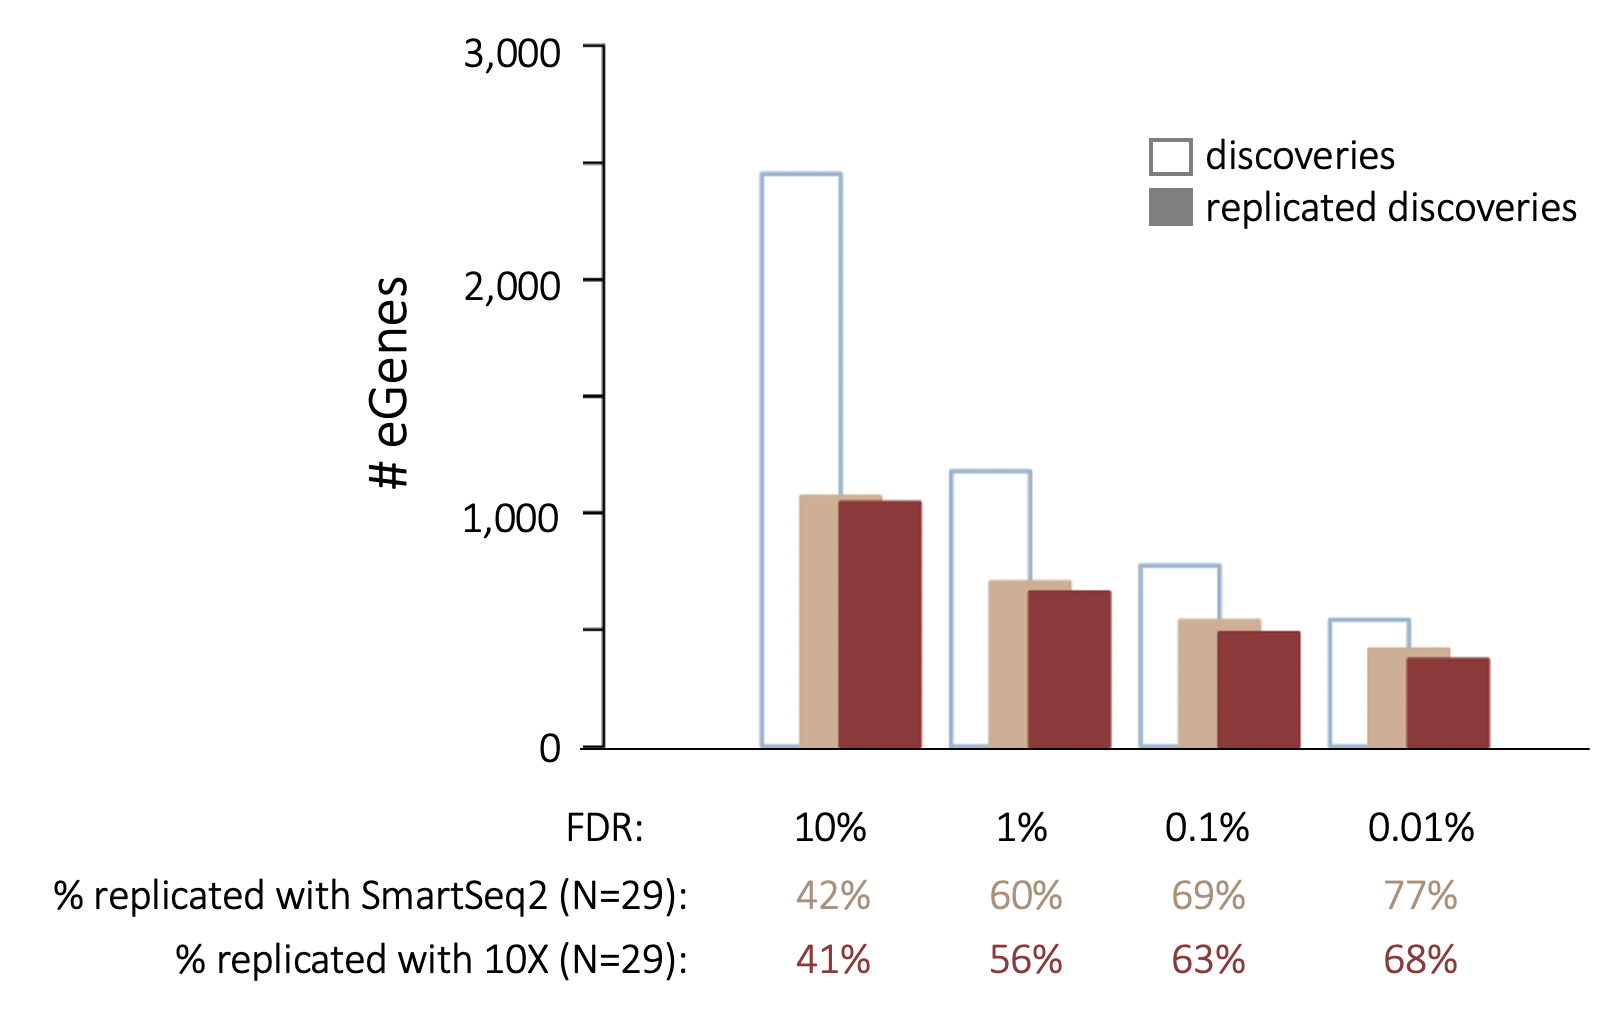
\includegraphics[width=14.5cm]{Chapter3/Fig/sc_vs_bulk_vs_10x.png}
\caption[iPSC bulk eQTL replication]{\textbf{Replication of iPSC bulk \gls{eqtl} using single cell across technologies}.\\
Replication of \gls{ipsc} \gls{eqtl} discovered with bulk RNA-seq (108 samples), using single cell RNA-seq data from a common set of 29 samples (SmartSeq2 in sand, 10X Genomics in red). 
The total number of bulk eGenes discovered is shown, along with the number of discoveries replicated using single cell profiles, at different FDR thresholds. 
As before, replication was defined as nominal significance, at p value < 0.05, and same direction of effect.}
\label{fig:sc_bulk_10x_egenes}
\end{figure}

\newpage

Additionally, we found good agreement in terms of effect sizes between the \gls{eqtl} maps obtained using the two different single cell technologies, highlighting the robustness of the approach (\textbf{Fig. \ref{fig:sc_eqtl_technologies}}). \\

\begin{figure}[h]
\centering
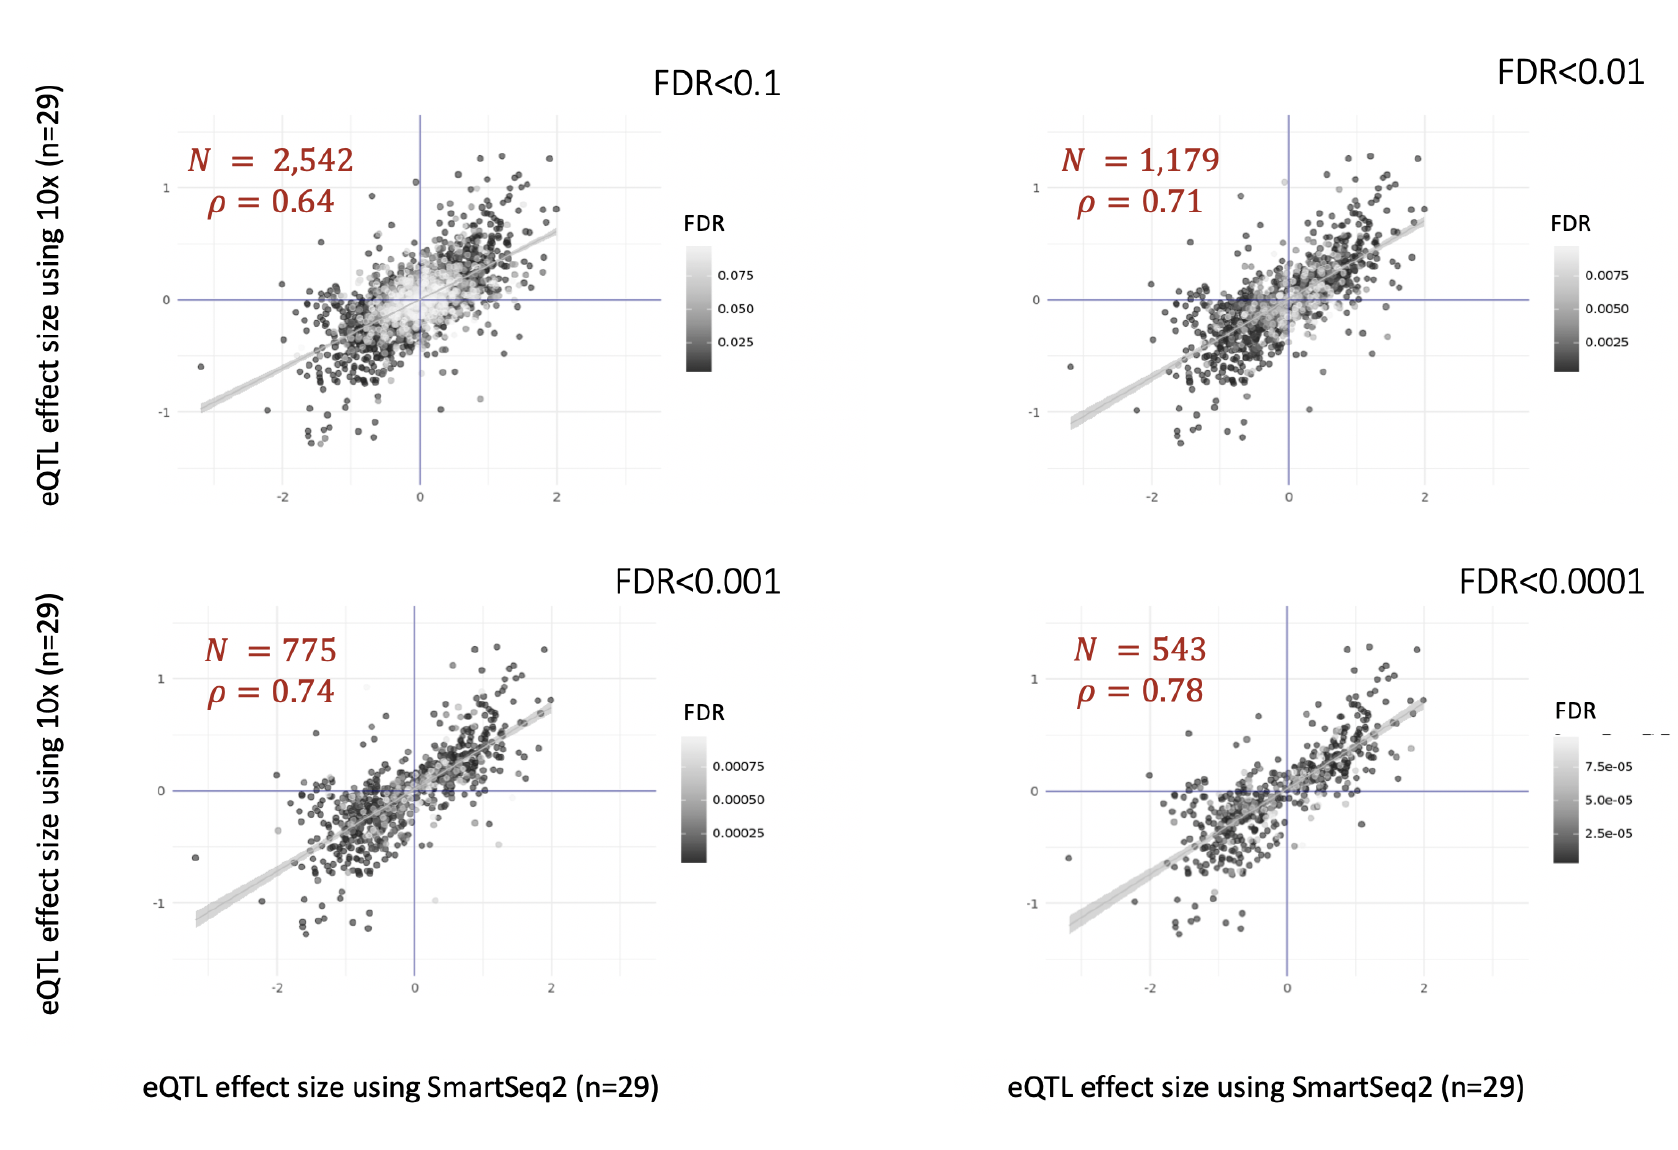
\includegraphics[width=15cm]{Chapter3/Fig/beta_comparison_ss2_vs_10x.png}
\caption[iPSC sc-eQTL replication across technologies]{\textbf{Effect size agreement between single cell technologies.}\\
Scatter plots of \gls{eqtl} effect sizes obtained when testing association of \gls{ipsc} \gls{eqtl} discovered using bulk RNA-sequencing (108 cell lines), using SmartSeq2 (\cite{picelli2013smart} x axis) and 10X Genomics (\cite{zheng2017massively} y axis) on cells from 5 experimental batches (experiments 31, 40, 41, 43, 44; 29 cell lines in total). 
The number of \gls{eqtl} examined and the correlation between effect sizes is indicated when we consider bulk \gls{ipsc} \gls{eqtl} discoveries at four different FDR thresholds (0.1, 0.01, 0.001, 0.0001).}
\label{fig:sc_eqtl_technologies}
\end{figure}

% As we acknowledge
Since the vast majority of scRNA-seq datasets presented recently use droplet-based (rather than plate-based) technology, as it allows, as we have seen (\textbf{page \pageref{fig:scrnaseq_plate_vs_droplet}}), the assessment of a much larger number of cells in a single experiment, it is important to show that this approach would work for such datasets as well. 
Whilst in this case we had data from too few individuals to make a very strong argument, the good concordance of results between 10X and SmartSeq2 suggests that this approach would work well for all single cell RNA-seq datasets, across technologies.

\clearpage

\section{Preliminary steps towards a best-practice pipeline}
\label{sec:best_practice}

The results presented so far are included in Cuomo \textit{et al}. \cite{cuomo2020single}, the other results of which I discuss in detail in the next chapter (\textbf{Chapter 
% 4
\ref{chapter4}}). \\

More recently, in collaboration with Marc Jan Bonder and Giordano Alvari from the Stegle group, I have worked on a best-practice pipeline which extends on the work presented so far, by testing the effect of different parameters of the model, to optimise yield of single cell eQTL mapping.
In particular, using the same iPSC data described so far (\textbf{Fig. \ref{fig:ipsc_data}}), we systematically compared results when mapping eQTL i) using various aggregation strategies to obtain `pseudo-bulk' expression levels to use as phenotypes in the model, and ii) varying the type and number of `global expression effect' covariates (see \textbf{section
\ref{sec:confounders}})
% 2.2.4}) 
that are included in the model.
% Finally, we evaluated normalisation strategies for the expression profiles used as phenotype.

\subsection{Overview of the iPSC data used}

As I have mentioned, we broadly use the same iPSC data as before, i.e. scRNA-seq from \cite{cuomo2020single} and (matched) bulk RNA-seq from the HipSci resource.
% rephrase this sentence
% However, we adopted a rather conservative approach with respect to the data included, to optimise this comparison. \\
However, we implemented some changes, to increase our confidence in this comparison. 
% \\
First, to make the data most comparable between the scRNA-seq data and the bulk RNA-seq data, we re-quantified single cell expression at the gene level using the `featureCounts' tool \cite{liao2014featurecounts}, as was done for the bulk RNA-seq data (rather than relying on the quantification using the pseudo-aligner salmon \cite{patro2017salmon}, which was used to obtain the results described above and all results in \textbf{Chapter \ref{chapter4}}).
% , which would have been inconsistent across technologies). 
\\

% Briefly, adapters were trimmed from reads using Trim Galore!, using default settings. 
% Trimmed reads were mapped to the human reference genome build 37 using STAR (version: 020201) in two-pass alignment mode, using the defaults proposed by the ENCODE consortium (STAR manual). 
% Gene-level RNA expression was quantified from the STAR alignments using featureCounts (v1.6.0), which was applied to the primary alignments using the `-B' and `-C' options in stranded mode if applicable, using the Ensembl 75 GTF file. \\

Additionally, to remove further possible confounding effects, a small group of lines from monogenic diabetes donors were excluded, as well as four lines which were slight outliers in the genotype space (\textbf{Fig. \ref{suppl_fig:kinship_pcs}}).
% excluded one line slightly off ethnicty-wise, other? i.e. at least X cells? (n=88?)
In total, we map single cell eQTL for 88 cell lines (from 88 donors).
As a cell QC step, we calculated the average correlation of each cell with all other cells.
Then, for each sequencing run, we calculated the median of the resulting cell-correlation values.
If a run had median cell-correlation < 0.7, all cells from the run were discarded (\textbf{Fig. \ref{fig:sc_eqtl_autocorrelation}}, panel a).
In a second step, cell-cell correlations were calculated again, between cells from the remaining runs only.
% All cells that had average correlation < 0.5 after this second step were also discarded (\textbf{Fig. \ref{fig:sc_eqtl_autocorrelation}}). 
This time, we considered line-run combinations, and discarded all combinations that had median cell-correlation < 0.5 (\textbf{Fig. \ref{fig:sc_eqtl_autocorrelation}}, panel b). \\

\begin{figure}[h]
\centering
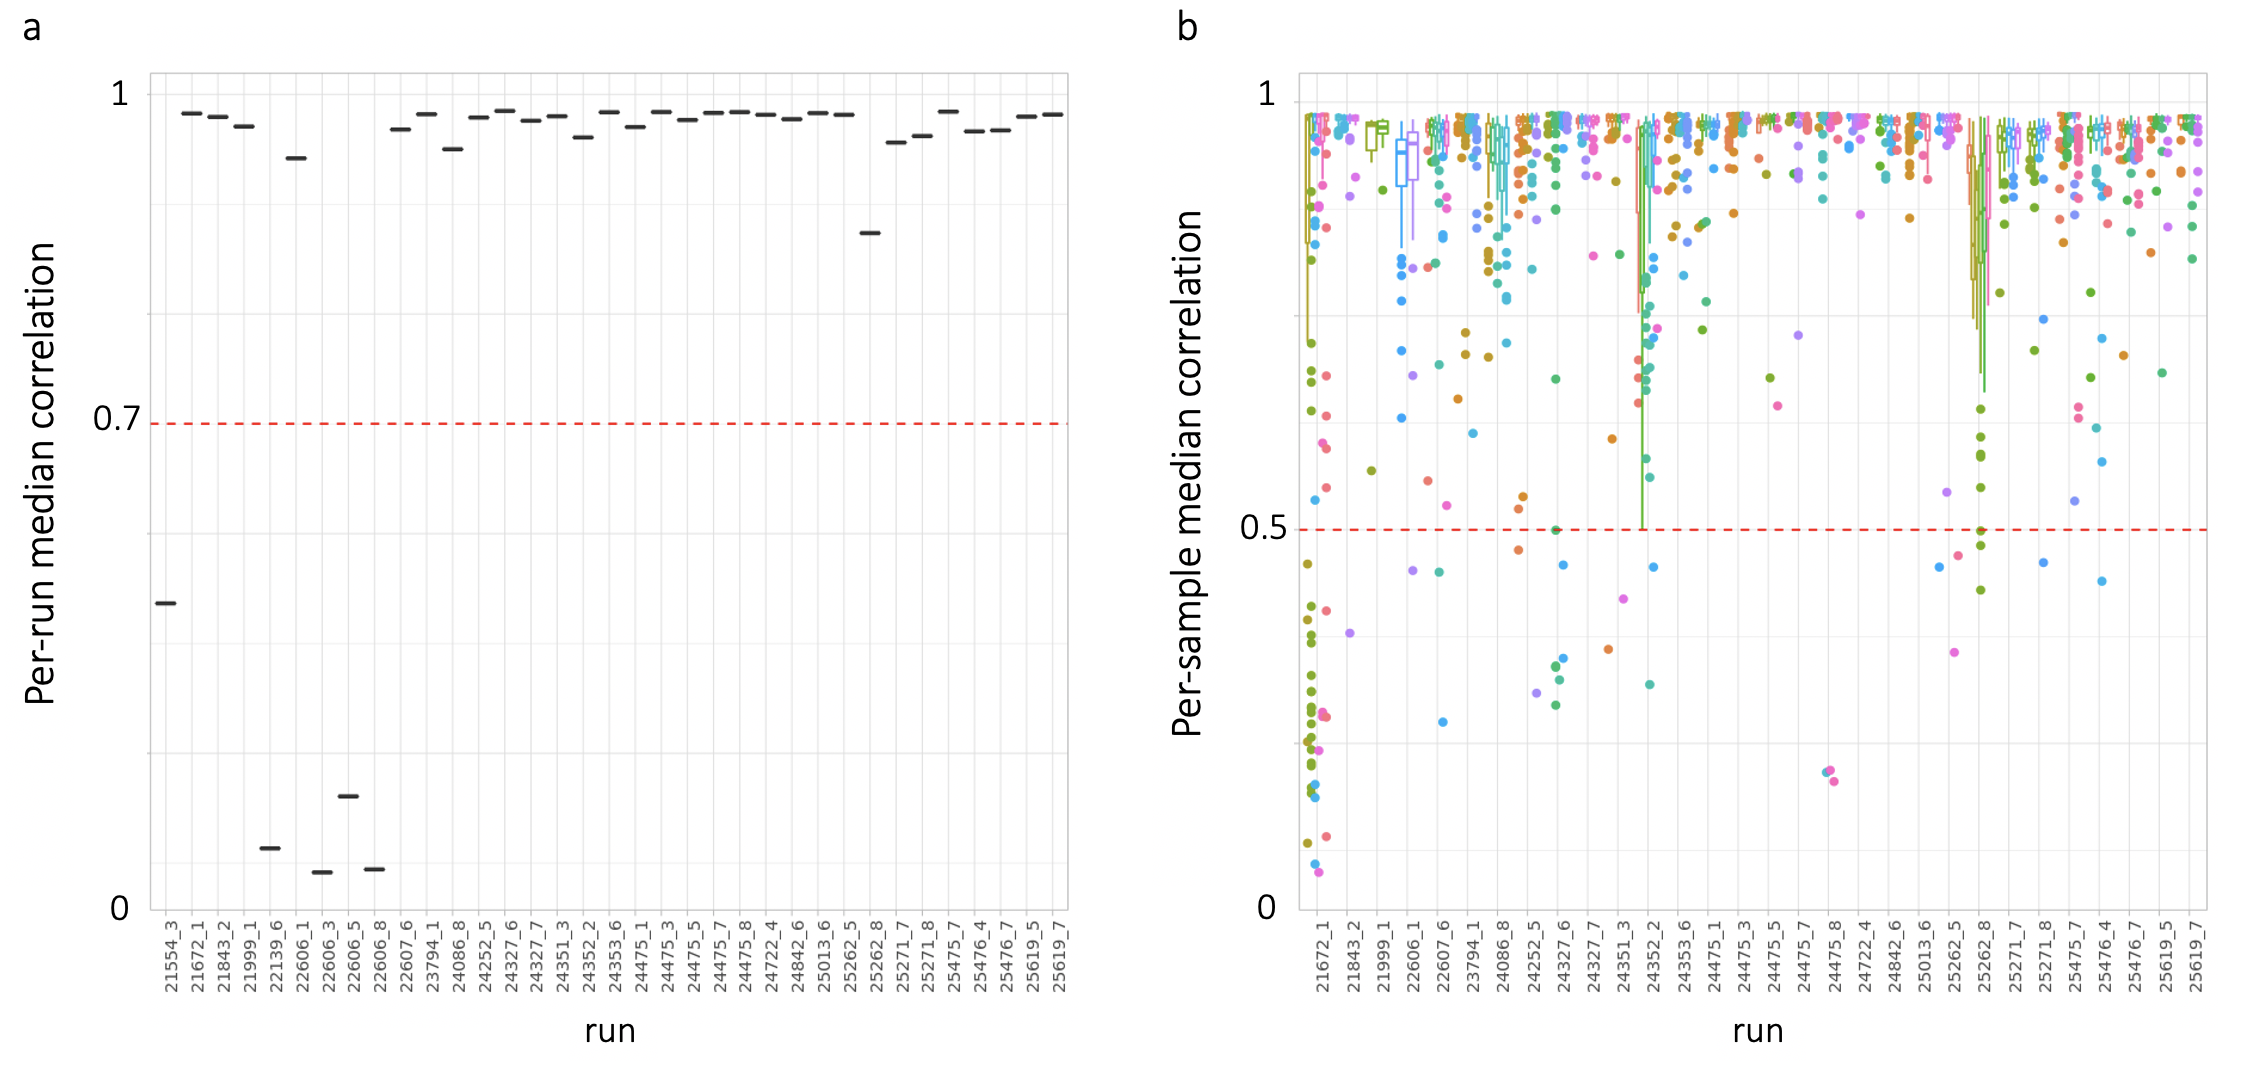
\includegraphics[width=15cm]{Chapter3/Fig/sc_eqtl_cell_QC.png}
\caption[Correlation-based cell QC]{\textbf{Correlation-based cell QC}\\
(a) Median cell-correlation calculated per run.
Runs with median cell-correlation < 0.7 were discarded.
(b) For the remaining runs, donor-run (i.e. sample) level median cell-correlations were calculated, and samples with median cell-correlation < 0.5 were discarded.}
\label{fig:sc_eqtl_autocorrelation}
\end{figure}

\newpage

Moreover, in order to compare eQTL results across genes at different expression levels, we chose to be more lenient on the criteria for gene inclusion.
% , such that we could test up to 50,425 genes in total. 
Indeed, we considered all variable genes as obtained by ranking all genes (n=50,425) by their squared coefficient of variation ($CV^2$)\footnote{$CV^2=\sigma^2/\mu^2$.} across all cells, and selecting the upper two quartiles.
As a result, 20,545 genes were included in the analysis. 
On the other hand, to reduce the multiple testing burden, we only tested SNPs with MAF >10\% and within a smaller window around the gene (100kb on either side of the gene body).

\subsubsection{Comparison partners}

Finally, we compared the resulting single cell eQTL maps with results obtained using bulk RNA-seq both limited to the same set of samples (n=88, `matched bulk'), and using all samples that were available at the time (n=810 HipSci lines from 527 unique donors, `bulk'). 

% % In order to produce bulk-like results, two main approaches can be used.

% % Under the assumption that we are looking at a single cell type, we can i) aggregate counts across all cells from an individual (e.g. taking the average expression value) and generate a `pseudo-bulk' measure, and then run the test exactly as if it were bulk; or ii) use full single cell expression, without aggregating.

% % % In this chapter, we introduce the two datasets that we will use throughout the thesis, setting the scene for all other chapters. 
% % % These are among the very first datasets of their kind, assessing single cell gene expression profiles for hundreds of genetically diverse individuals, allowing to interrogate the effect of common genetic variation on transcriptional variability.
% % % Previously, most \gls{eqtl} mapping studies in humans were performed using bulk RNA-sequencing, and most scRNA-seq studies were performed in a handful of individuals only, or in model organisms (often also limited to a few strains).
% % % Notably, one study performed \gls{eqtl} mapping using scRNA-seq \cite{van2018single} recently in blood cells. 
% % % However, this data is limited to 45 individuals and to a single time point, lacking the differentiation axis of our studies.

% % % \subsection{Datasets}

% % % \begin{itemize}
% % %     \item iPS data
% % %     \item simulated data
% % % \end{itemize}

% % \subsection{Data}

% % We use iPS data from \cite{cuomo2020single} - day0 only, etc

% % Smartseq2 \cite{picelli2013smart} data from 10,000 (get exact number) cells from 112 unique unrelated donors, across YY differentiation experiments. 

\newpage

\subsection{Aggregation strategies}

% Add something about sum vs mean, what's more obvious, bla bla normalisation + batch effects and whether to aggregate by donor or not..
% Introduce this. 
% Also repeat this is after cell type identification and QC.\\

% Pseudobulk approach.
As a first step, we investigated which aggregation method (aimed at summarising single cell values to a `pseudobulk' level) resulted in the most power to identify single cell \gls{eqtl}.

To do so, we tested the following approaches:

\begin{itemize}
    \item \textbf{Mean}: average expression across cells from each donor and sequencing run\footnote{This is very similar to the approach used in the first part of this chapter, i.e. using the same principle of accounting for batches.
    The difference is that this is done at an even deeper level of batch, i.e. cells from the same experimental pool were sometimes sequenced in more than one run.},
    \item \textbf{Median}: median expression across cells from each donor and sequencing run,
    \item \textbf{Sum}: summed expression across cells from each donor and sequencing run,
    \item \textbf{Total mean}: average expression across all cells from each donor, aggregated across sequencing runs, and finally
    \item \textbf{Total sum}: similar to the total mean, but summing reads instead.
\end{itemize}

% \newpage

For the first three methods, aggregation is done not only at the donor level but also for each individual sequencing run (i.e. all iPS cells from a given donor in a single sequencing run), to account for possible batch effects (see \textbf{page \pageref{sec:sc_ipsc_eqtl}}).
% This is done in an attempt to account for batch effects (needs explaining).
For what we call `total' sum and mean, on the other hand, aggregation (i.e. sum or mean) is done at the donor level only, to maximise the numbers of cells per donor.
In all cases (i.e. using any of the aggregation methods) aggregated expression values were only calculated for samples (i.e. donors or donor-run combinations) with at least 5 cells.

\subsection{Normalisation strategies}

Importantly, normalisation of the scRNA-seq data was performed in different ways depending on the aggregation method used.
For mean (including total mean) and median aggregation of expression data, we performed single cell-level normalisation using two alternative methods, i) scran/scater \cite{mccarthy2017scater} size factor normalisation and ii) baynorm \cite{tang2020baynorm}.
% Briefly, log2(cpm+1) using size factors..
The mean and the median were then calculated on the resulting normalised (logged) counts (\textbf{Fig. \ref{fig:sc_qtl_workflow}}). \\

On the other hand, summed count values (both sum and total sum) were obtained directly from the un-normalised data.
Normalisation was then applied on the resulting pseudo-bulk counts, using methods typically used for bulk RNA-seq data.
In particular, we perform (logged) CPM normalisation using edgeR \cite{robinson2010edger}, accounting for library size (\textbf{Fig. \ref{fig:sc_qtl_workflow}}).

\begin{figure}[h]
\centering
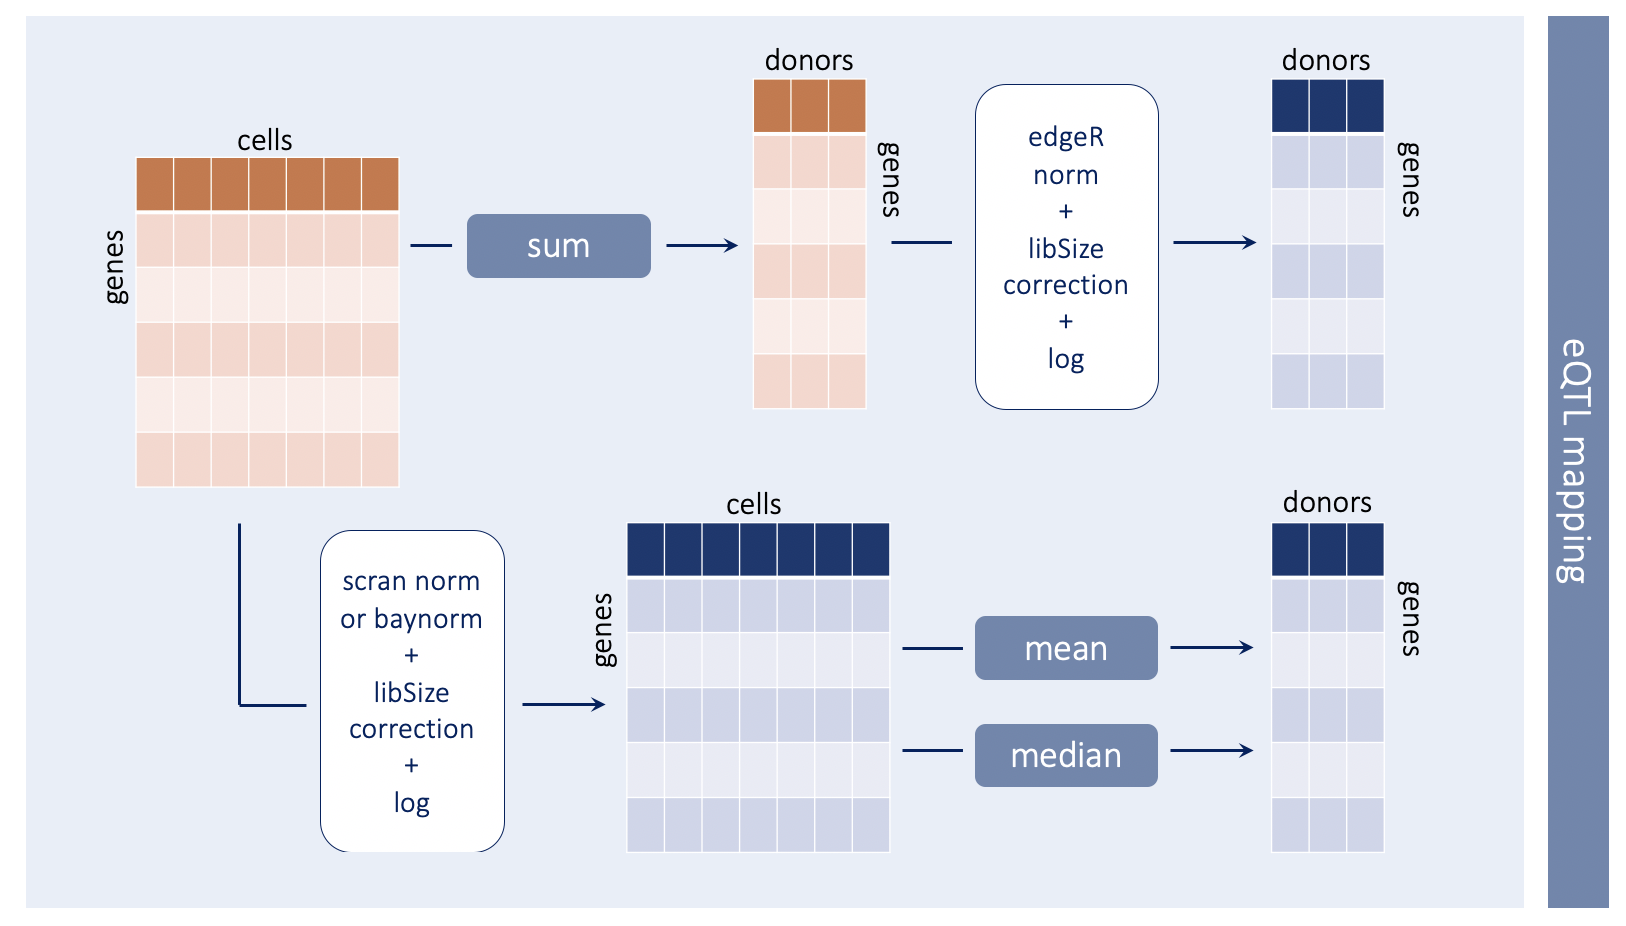
\includegraphics[width=16cm]{Chapter3/Fig/sc_qtl_workflow_no1_2_steps.png}
\caption[sc-eQTL workflow]{\textbf{sc-eQTL workflow}.\\
Different approaches tested to perform \gls{eqtl} mapping using scRNA-seq profiles.
% After processing and QC, and after a homogeneous cell population has been identified (1), and checking across samples correlation i.e. if very low across all genes, may be the wring cell type (2), one count matrix (cells x genes). 
Starting from one gene $\times$ cell count matrix, counts were aggregated per sample (i.e. donor, or donor-run combination), either by summing the data first at sample-level and then normalising using methods designed for bulk RNA-seq (i.e. edgeR \cite{robinson2010edger}) or by first normalising the single cell counts (using scran/scater \cite{mccarthy2017scater} or baynorm \cite{tang2020baynorm}) and then calculating the mean or the median at the sample-level. }
\label{fig:sc_qtl_workflow}
\end{figure}

\subsection{Phenotype transformation}

Linear (mixed) models assume normality of the phenotype vector $\mathbf{y}$ (\textbf{Chapter
\ref{chapter2}}).
% 2}).
However, when using gene expression, we are in the presence of count data.
By log-transforming (log2) and normalising (previous section) such counts, the model-fit is improved, yet this approach still remains sub-optimal (see \textbf{section \ref{sec:non_gaussian}}). \\

In addition, two commonly-used phenotype transformations include standardising each phenotype vector (as I have done before) or quantile-normalising it, i.e. ranking the values and then making the data fit to a Gaussian distribution, forcibly.
Here, we chose the latter strategy, which is more conservative, as it ensures a better fit to the (Gaussian) model.
This approach often results in slightly reduced power but it is more robust, thus better suited for this comparison.

\subsection{Comparing sc-eQTL results across aggregation approaches}

Next, the (normalised and `gaussianised') aggregated expression values resulting from each of the methods described were used to map eQTL.
For this comparison, the first 20 principal components were calculated from each of the aggregated matrices and included in the model as covariates (as before, from eq. \eqref{eq:LMM_ipsc_eqtl}, P = 20).
% Finally, variable genes were obtained by ranking all genes by their squared coefficient of variation ($CV^2$)\footnote{$CV^2=\sigma^2/\mu^2$.} across all cells, and selecting the upper two quartiles (20,545 genes), which were included in the analysis. 
% As mentioned, the aggregated expression values for each of these genes were quantile-normalised and plugged into the pipeline (eq. \eqref{eq:LMM_ipsc_eqtl}), one at a time. 
\\

% \clearpage

\textbf{Table \ref{tab:egenes}} summarises the results across the aggregation methods tested, when restricting the results to the set of 13,167 genes that were tested in each of the eQTL maps.
The comparison is first of all in terms of yield, i.e. number of eGenes identified using each of the methods.
Next, we assess the degree of replication of the discoveries in the set of results obtained using bulk RNA-seq, both using matched samples only, and using all samples.\\

% We observe that the method that performs best is the mean, both in terms of discoveries and consistency with bulk (Table \ref{tab:egenes}).\\

% Results not on common genes, using Giordano's selection:

% \begin{table}[h]
%     \centering
%     \begin{tabular}{c|c c c c c}
%     & \# eGenes & genes tested & \% significant & \% matched bulk  & \% bulk   \\
%     \hline
%     mean         & 2,081 & 20,545 & 10.1\% & 58\% & 71\% \\
%     total mean   & 1,363 & 19,877 & 6.9\% & 66\% & 76\% \\
%     median       & 1,530 & 13,567 & 11.3\% & 48\% & 61\% \\
%     sum          & 1,598 & 20,545 & 7.8\% & 65\% & 75\% \\
%     total sum    & 1,291 & 20,545 & 6.3\% & 66\% & 76\% \\
%     matched bulk & 1,557 & 20,336 & 7.7\% &  - & 97\% \\
%     bulk         & 8,751 & 20,541 & 43\% & - & - \\
%     \end{tabular}
% \end{table}

% Results not on common genes, using Anna's selection:

% \begin{table}[h]
%     \centering
%     \begin{tabular}{c|c c c c c}
%     & \# eGenes & genes tested & \% significant & \% matched bulk  & \% bulk   \\
%     \hline
%     mean         & 1,557 & 10,767 & 14.5\% & 53\% & 70\% \\
%     total mean   & 1,021 & 10,408 & 9.8\% & 62\% & 75\% \\
%     median       & 1,158 & 10,227 & 11.3\% & 53\% & 67\% \\
%     sum          & 1,226 & 10,768 & 11.4\% & 61\% & 74\% \\
%     total sum    & 944 & 10,767 & 8.7\% & 64\% & 78\% \\
%     matched bulk & 790 & 10,766 & 6.3\% &  - & 98\% \\
%     bulk         & 5,093 & 10,772 & 47\% & - & - \\
%     \end{tabular}
% \end{table}

% \newpage

% Common genes (mean, totmean, median, sum, totsum): 13,177,
% including (matched) bulk too: 13,167.

% In Giordano's selection: 13,167.

% In Anna's selection: 9,886.


\begin{table}[h]
    \centering
    \begin{tabular}{c|c c c c c}
    & \# eGenes & genes tested & 
    \% genes tested & 
    % \multicolumn{1}{>{\centering}m{2cm}}{\% genes tested} &
    \multicolumn{1}{>{\centering}m{2.3cm}}{\% replicated in matched bulk} & \multicolumn{1}{>{\centering}m{2.22cm}}{\% replicated in bulk} \\
    % & & & & \% replicated & \% replicated \\
    % & \# eGenes & genes tested & \% genes tested &  matched bulk & bulk \\
    %  \\
    \hline
    mean         &  1,831 & 13,167 & 13.9\% & 66\% & 76\% \\
    total mean   &  1,309 & 13,167 &  9.9\% & 73\% & 81\% \\
    median       &  1,486 & 13,167 & 11.3\% & 55\% & 66\% \\
    sum          &  1,434 & 13,167 & 10.9\% & 70\% & 81\% \\
    total sum    &  1,153 & 13,167 &  8.8\% & 73\% & 82\% \\
    matched bulk &  2,683 & 13,167 & 20.4\% & - & 95\% \\
    bulk         &  9,983 & 13,167 & 75.8\% & - & - \\
    \end{tabular}
    \caption[Aggregation method comparison]{\textbf{Aggregation method comparison.}\\
    For various aggregation methods (rows), and using 20 PCs as covariates, indicated are the total number of eGenes, the percentage of eGenes out of the genes tested (13,167), the percentage of eGenes for which the lead eQTL is replicated when mapping eQTL using bulk RNA-seq with only matched samples (n=88, `matched bulk'), and using all samples (810 lines, 527 donors, `bulk').
    Discoveries using bulk were also added, for reference (last two rows).}
    \label{tab:egenes}
\end{table}



% % The results presented in Table \ref{tab:egenes} are when testing all 20,545 genes (as described above).
% When considering only the 10,408 genes tested above (and presented in \cite{cuomo2020single} and in Chapter 4), the results were equivalent, where we note that yield and bulk replication both are relatively higher when we only consider genes expressed in at least xx cells (Table \ref{tab:egenes_annas_selection}).

% \begin{table}[h]
%     \centering
%     \begin{tabular}{c|c c c c }
%     & \# eGenes & \% genes tested & \% matched bulk  & \% bulk   \\
%     \hline
%     mean         & 1,381 & 13.3\% & \% & \% \\
%     total mean   & 853 & 8.2\% & \% & \% \\
%     median       & 1,106* & 11.2\%* & \% & \% \\
%     sum          & 1,045 & 10.0\% & \% & \% \\
%     total sum    & 797 & 7.7\% & \% & \% \\
%     matched bulk &  & \% & - & \% \\
%     bulk         &  & \% & - & - \\
%     \end{tabular}
%     \caption[Aggregation method comparison, genes from Cuomo \textit{et al.} only]{Same as Table \ref{tab:egenes},  but when only testing the genes selected previously (and assessable in each of these maps, n=10,408 genes).
%     *median testing only 9,886 genes.}
%     \label{tab:egenes_annas_selection}
% \end{table}

These results indicate that considering the mean as the aggregation method is the optimal approach, resulting by far in the most eGenes identified (\textbf{Table \ref{tab:egenes}}).
In terms of replication of bulk results (measured as nominal significance and same direction of effects), the mean results are comparable with the sum, total sum, and total mean, whereas the median, which performed quite well in terms of yield, had substantially fewer of its identified eQTL replicated using bulk. 
Here we note that, although in terms of percentage total mean and total sum outperform the mean, since the number of eGenes is higher, the mean is also the method that identifies the most eGenes replicated in bulk (1,397 vs 1,155 for the second best, the sum). \\

We speculate that whilst the sum would perhaps be the most obvious approach to reproduce bulk-like measurements, the mean might perform better because of the normalisation used.
Indeed, the normalisation at the cell-level may better balance the differences in read counts across cells prior to the aggregation at individual-level. 
Next, we also tested an alternative single cell normalisation approach, baynorm \cite{tang2020baynorm}, and mapped eQTL using the mean aggregation method, finding that the results were virtually indistinguishable (1,834 eGenes vs 1,831, and Pearson's correlation between both p values and effect sizes: R=1, p value < 2.2$\times 10^{-16}$, \textbf{Fig. \ref{suppl_fig:scran_vs_baynorm}}). \\

Reassuringly, we broadly replicated the key results found in the first part of this chapter, confirming that eQTL maps using bulk RNA-seq are better powered that those using single cells, at identical sample size.
Additionally, mean and sum (i.e. aggregating at donor and batch) outperformed total mean and total sum (\textbf{Table \ref{tab:egenes}}), re-iterating the importance of considering replicated experimental designs for eQTL studies.

% add here maybe ROC curve etc

% \clearpage

\subsection{Comparing results using different expression covariates}

% Expression covariates PCs, PEER established (add references, e.g. GTEx..)

As a second comparison, we varied the type and number of expression covariates included in the model to account for global expression variation (see \textbf{section 
\ref{sec:confounders}}).
% 2.2.4}).
Since the mean outperformed other aggregation methods, we only perform this comparison using mean-aggregated values.
Indeed, we computed principal components (PCs), MOFA factors \cite{argelaguet2018multi}, PEER factors \cite{stegle2010bayesian,stegle2012using} and single value decomposition (SVD) from the mean expression matrix. 
% \\
Next, we included 5, 10, 15, 20 and 25 PCs, MOFA, PEER and SVD factors in the model (eq. \eqref{eq:LMM_ipsc_eqtl}) as covariates, and mapped eQTL.
In a first instance, we compared results when running these maps for chromosome 2 genes only (1,421 genes). \\

To evaluate performance, as before, we first considered the number of eGenes (\textbf{Table \ref{tab:covariates}}):


% PCs/PEER/SVD:
% 3,764 genes in total
% 1,423 in G's selection
% 726 in A's selection
% (for MOFA 3,809 genes in total, filtered down)

% \begin{table}[h]
%     \centering
%     \begin{tabular}{c|c c c c c}
%     &         5 & 10 & 15 & 20 & 25  \\
%     \hline
%     PCA   & 10.0\% & 11.1\% &  12.9\% & 12.3\% & 11.6\%  \\
%     MOFA  & 6.7\% & 7.5\% &  8.4\% & 8.8\% & -  \\
%     PEER  & 9.6\% & 8.9\% &  9.4\% & 8.2\% & -  \\
%     SVD  & 11.1\% & 11.1\% &  12.0\% & 11.7\% & 11.2\% \\
%     \end{tabular}
%     \caption[Number and type of covariate comparison]{Number of eGenes for various types and numbers of covariates. 
%     Out of 1,421 (chromosome 2) genes tested.
%     Mean as aggregation method.}
%     \label{tab:covariates}
% \end{table}

\begin{table}[h]
    \centering
    \begin{tabular}{c|c c c c c}
    &       5 & 10 & 15 & 20 & 25  \\
    \hline
    PCA   & 160 & 155 &  184 & 175 & 168 \\
    MOFA  & 122 & 138 &  142 & 148 & -   \\
    PEER  & 146 & 139 &  146 & 126 & -   \\
    SVD   & 179 & 177 &  171 & 166 & 160 \\
    \end{tabular}
    \caption[Number and type of covariate comparison]{\textbf{Number of eGenes for various types and numbers of covariates.}\\
    Rows are methods to calculate covariates, columns number of covariates considered for the eQTL test.
    The numbers of eGenes are to be considered out of 1,421 (chromosome 2) genes tested.
    The mean is used as aggregation method, normalised using scran.}
    \label{tab:covariates}
\end{table}

% \begin{table}[h]
%     \centering
%     \begin{tabular}{c|c c c c c}
%     &         5 & 10 & 15 & 20 & 25  \\
%     \hline
%     PCA   & 142 (10\%) & 158 (11\%) &  184 (13\%) & 175 (12\%) & 165 (12\%)  \\
%     MOFA  & 96 (7\%) & 107 (8\%) &  119 (8\%) & 125 (9\%) & -  \\
%     PEER  & 137 (10\%) & 126 (9\%) &  134 (9\%) & 116 (8\%) & -  \\
%     linear SVI  & 158 (11\%) & 159 (11\%) &  171 (12\%) & - & 160 (11\%) \\
%     \end{tabular}
%     \caption[Number and type of covariate comparison]{Number of eGenes for various types and numbers of covariates. 
%     Out of 1,423 (chromosome 2) genes tested.
%     Mean as aggregation method.}
%     \label{tab:covariates}
% \end{table}

% \begin{table}[h]
%     \centering
%     \begin{tabular}{c|c c c c c}
%     &         5 & 10 & 15 & 20 & 25  \\
%     \hline
%     PCA   & 13.0\% & 14.2\% &  16.5\% & 16.4\% & 16.9\%  \\
%     MOFA  & 8.3\% & 9.9\% &  11.7\% & 11.0\% & -  \\
%     PEER  & 14.2\% & 11.0\% &  12.1\% & 11.0\% & -  \\
%     SVD  & 15.3\% & 14.7\% &  18.2\% & - & 17.1\% \\
%     \end{tabular}
%     \caption[Number and type of covariate comparison]{Number of eGenes for various types and numbers of covariates. 
%     Restricted to the 726 (on chromosome 2) from my previous selection.
%     Mean as aggregation method.}
%     \label{tab:covariates_annas_selection}
% \end{table}


% \begin{table}[h]
%     \centering
%     \begin{tabular}{c|c c c c c}
%     &         5 & 10 & 15 & 20 & 25  \\
%     \hline
%     PCA   & 69.4\% & 73.6\% &  69.9\% & 70.3\% & 68.5\%  \\
%     MOFA  & 80.8\% & 74.6\% &  77.5\% & 77.0\% & -  \\
%     PEER  & \% & \% &  \% & \% & -  \\
%     SVD   & \% & \% &  \% & \% & \% \\
%     \end{tabular}
%     \caption[Covariate comparison in terms of replication of bulk results]{Number of bulk-replicated eGenes for various types and numbers of covariates. 
%     Same as Table \ref{tab:covariates_replication}, but considering replication in the set of results using bulk (all samples, p value < 0.05 and same direction of effect).}
%     \label{tab:covariates_replication}
% \end{table}

Next, we considered the number of eQTL that were replicated using bulk (using all samples, nominal significance and same direction of effect, \textbf{Table \ref{tab:covariates_replication}}, for the equivalent results using `matched bulk' see \textbf{Table \ref{tab:covariates_replication_matched_bulk}}):

\begin{table}[h]
    \centering
    \begin{tabular}{c|c c c c c}
    &         5 & 10 & 15 & 20 & 25  \\
    \hline
    PCA   & 118 & 128 & 136 & 136 & 128 \\
    MOFA  & 103 & 113 & 119 & 122 &  -  \\
    PEER  & 111 & 107 & 115 &  99 &  -  \\
    SVD   & 139 & 134 & 129 & 127 & 126 \\
    \end{tabular}
    \caption[Covariate comparison in terms of replication of bulk results]{\textbf{Number of bulk-replicated eQTL for various types and numbers of covariates.} \\
    Similar to \textbf{Table \ref{tab:covariates}} (mean as aggregation method, 1,421 chromosome 2 genes only), but considering replication in the set of results using bulk (all samples, p value < 0.05 and same direction of effect).}
    \label{tab:covariates_replication}
\end{table}

% Add same but in terms of bulk replication
Overall, we observe that in this application the two arguably simplest methods, PCA and SVD, slightly outperform other methods.
However, we note that this choice may depend more on the data used.
For example, PEER allows to incorporate known covariates, which in some cases (e.g. large group effects) may increase performance.
Additionally, the values of both MOFA and PEER factors depend on some of the settings such as sparsity, and number of factors imputed, which we have yet to optimise.
Nevertheless, at the very least PCA performs as well as other methods, particularly here, where the cell population is homogeneous and the batch effects are minimal (and addressable, thanks to the replicated design).
In particular, the ideal number of PCs to include seems to be 15-20 (\textbf{Tables \ref{tab:covariates}, \ref{tab:covariates_replication}}). 
\\

In summary, our recommendation for optimising yield of eQTL mapping using single cell expression profiles is to normalise counts at the cell-level, using single cell specific methods such as scran \cite{lun2016step}(or baynorm \cite{tang2020baynorm}, which performed similarly well), then aggregate such counts by considering the mean expression across cells.
Depending on the experimental design, if data from a given donor is present across multiple technical batches, we recommend considering those batches as separate replicates for the donor, and calculating the mean for the two separately.
Next, principal components can be calculated from such aggregated expression matrix, and the first 15-20 PCs should be included as covariates in the model.
We also acknowledge that the number of PCs to include will depend on the sample size of the study.
For example, in the case of several hundreds of individuals, 25 or 50 PCs may be more appropriate. 

\newpage

Future work towards establishing a best-practice pipeline for single cell eQTL studies includes confirming such recommendations using droplet-based data, for example data I will introduce in \textbf{Chapter 
% 5
\ref{chapter5}}, which have been sequenced using the 10X Genomics Chromium technology \cite{zheng2017massively}. 
Moreover, future avenues involve the use of experimental-data informed simulation experiments to assess the impact of additional variables including varying numbers of cells per donor, varying sample size, batch effects and genetic effects of varying strength, on our ability (and statistical power) to detect eQTL using single cell expression data.

% \clearpage

\section{Discussion}

Since being highlighted as `Method of the Year' in 2013 \cite{editorial2014method}, sequencing of the genetic material of single cells has become common-practice to investigate cell-to-cell heterogeneity in biological systems \cite{lahnemann2020eleven}. 
In particular, 
% single-cell RNA sequencing (scRNA-seq) 
\gls{scrnaseq}
enables the quantification of gene expression  transcriptome-wide, and at single-cell resolution, allowing for cell type sub-populations to be distinguished \cite{anchang2016visualization, young2018single, muraro2016single, ernst2019staged, pijuan2019single, velten2017human},
and the identification of cells transitioning between states \cite{la2018rna, buettner2015computational, trapnell2014dynamics, bendall2014single, moignard2015decoding}. \\

Now an established method, \gls{scrnaseq} can be extended to profile single cell expression across several individuals, enabling the study of the effect of different genetic backgrounds on gene expression, at single cell resolution.
Single cell \gls{eqtl} (or as they called them scQTLs) were first introduced in a paper by Wills \textit{et al.}, in 2013 \cite{wills2013single}.
In their paper, the authors study lymphoblastoid cell lines from only 15 donors, but could already observe some cell type-specific effect, which could not have been identified using bulk profiling.
In 2018, Van der Wijst \textit{et al.} \cite{van2018single} published the second sc-\gls{eqtl} map, this time across blood cell types from 45 individuals.
They showed consistent direction of effects compared to bulk \gls{eqtl} on similar cell types, but could only replicate a very small percentage of the bulk-identified \gls{eqtl} ($\sim$10\%). \\
% (8\% and 11\%)

The work I present in this chapter (and in the next, and published in \cite{cuomo2020single}) was the third effort to map \gls{eqtl} using \gls{scrnaseq} profiles, and the best powered at the time, with data from over one hundred individuals.
Additionally, the use of bulk and \gls{scrnaseq} data from matched samples makes this the first step towards a systematic assessment of the differences between bulk and single-cell transcriptomics, as applied to \gls{eqtl} mapping.
As I have shown, compared to the results from \cite{van2018single}, we could replicate approximately 50\% of the \gls{eqtl} found using bulk, and almost all of the strongest signals (\textbf{Fig. \ref{fig:sc_bulk_egenes}}). \\

% maybe would add results of the second part here?
Our preliminary results on a best-practice workflow for sc-eQTL studies suggest that mean is the preferable aggregation method, probably due to data normalisation considerations.
% scran normalisation similar in performance to baynorm..
Additionally, PCA slightly outperforms other linear matrix decomposition approaches for correcting for global expression covariates.
Future work includes validating these results when mapping eQTL using 10X data, where we expect normalisation to have an even larger impact, due to the increased sparsity of the data.
Moreover, the use of real data-informed simulations will allow a more extensive power analysis, as their use will enable us to scale up the numbers of donors and cells and introduce group structure to comprehensively investigate the role of those parameters as well.
\\

Yet, altogether, the results from this chapter illustrate a difference between bulk and single-cell \gls{eqtl} mapping: there is a trade-off between statistical power and cellular resolution. 
Indeed, in this analysis of iPS cells, bulk RNA-seq data provided higher statistical power for discovery of \gls{eqtl} (about 30\% more discoveries using bulk). 
However, \glspl{ipsc} are a very homogeneous cell type.
% , thus bulk RNA-seq is well suited to 
In more heterogeneous populations of cells, such as cells in the brain, the single cell transcriptomes may become critical for defining pure populations, thus increasing power to detect \gls{eqtl}.\\

A further advantage of the application of single-cell RNA-seq data in this study, was to enable the pooled experimental design. 
Indeed, this setup allows us to assay cells from many individuals in a single, neatly contained, experiment.
As single-cell approaches are extended to more disease-relevant tissues and cell types, this may provide important clues on the causal role of genetic variants in disease. \\

These future studies are likely to be using droplet-based technologies, which allow the assessment of a much larger number of cells.
Although our main results are on (plate-based) SmartSeq2 data, we could validate our approach with a subset of samples assayed with the droplet-based 10X Genomics technology (\textbf{Fig. \ref{fig:sc_bulk_10x_egenes}}), which is a strong indication that single cell \gls{eqtl} mapping can be performed using droplet-based \gls{scrnaseq} data. \\

Finally, in this chapter we have focused on reproducing standard `mean' expression level \gls{eqtl} mapping using \gls{scrnaseq}, where the phenotype of interest is expression abundance within a homogeneous population of cells.
We can call such efforts `pseudo-bulk' approaches, where we are essentially replicating bulk-like expression values and performing the \gls{eqtl} test adapting approaches used for traditional \gls{eqtl} mapping using bulk RNA-seq. 
In the applications we and others have described \cite{van2018single,cuomo2020single}, the value of using \gls{scrnaseq} lies in the fact that we are able, within a single experiment, to unbiasedly define and map eQTL in multiple different cell types, whilst retaining a single cell resolution.\\

Now that we have established that such `mean-level' \gls{eqtl} maps are feasible, new \gls{eqtl} analyses, that specifically exploit the single cell resolution, can be performed (\textbf{Fig. \ref{fig:sc_eqtl}}).
One such analyses is variance \gls{eqtl} (varQTL, vQTL \cite{ayroles2015behavioral}) mapping, where one can assess the effect of common genetic variants on cell-to-cell transcriptional variability, rather than on expression abundance.
Unfortunately, these analyses have proven especially challenging, largely because the variance of gene expression is strongly dependent on its mean, making it hard to disentangle the two effects \cite{vallejos2016beyond}.
Moreover, variance QTL effects may be smaller than anticipated.
As a result, studies at current sample sizes are under-powered to detect any variance QTL, as 
% we (not shown) and others
shown by \cite{sarkar2019discovery}. \\

On the other hand, a single-cell approach allows detailed annotation of changing \gls{eqtl} effects across heterogeneous cell types and cell states, with the ability to better interpret the context-specific role of individual genetic variants. 
In particular, dynamic \gls{eqtl}, where the effect of a genetic variant on gene expression is modulated by differentiation time \cite{francesconi2014effects, strober2019dynamic} can be extended to single cell-resolved data, and expanded to include not only differentiation trajectories, but any cellular state.
In the next chapter (\textbf{Chapter 
\ref{chapter4}}),
% 4}), 
I will present examples of dynamic \gls{eqtl} and \gls{eqtl} affected by other cellular contexts.
%!TEX root = ../thesis.tex
%*******************************************************************************
%****************************** Fourth Chapter *********************************
%*******************************************************************************

\chapter{Mean level eQTL mapping using single cell RNA-seq}

In this chapter we continue the analyses on the datasets described in Chapter 3 and add in the genetic variation aspect; we can now adapt the LMM-based methods traditionally used for eQTL mapping (described in Chapter 2) to single cell data. 
In particular, we validate our method (focusing on the iPS cells) by systematically comparing eQTL results we obtained using single cells to eQTL identified using bulk RNA-sequencing (section 4.2). 
In addition, we compare eQTL results obtained when using two alternative single cell technologies: a plate-based (SmartSeq2) and a droplet-based (10X Genomics) technology, for a subset of lines (section 4.3). 
Finally, we perform eQTL maps of the mesendoderm and definitive endoderm stages (section 4.4), and of various stages of neuronal development (section 4.5) all of which are novel to this study to the best of our knowledge. 
The key results described in this chapter are contained in (Cuomo et al, 2020, Alvari, Cuomo et al, 2020, Jerber, Seaton, Cuomo et al, 2020).

\section{What is different in single cell data?}

When we perform eQTL mapping, we are interested to find differences in expression level between individuals, as a function of their different genotypes as specific genomic loci. 
Under the assumption that we are looking at an otherwise homogeneous population of cells (e.g. all cells of a given cell type) it is reasonable to take the sum or the average expression per individual, across all cells.
When we use bulk RNA sequencing expression profiles, that is essentially what happens. 
All cells from an individual are pooled, the mRNA extracted and sequenced. 
The resulting reads are and mapped onto a reference genome, and the expression level of each genes is quantified as the number of reads obtained from one donor that uniquely map to that gene. 
A bulk RNA-seq experiment, therefore, results in one individual measure of “abundance” of each gene for each donor. 
Such measure is the results of aggregating over XX cells [REF] and, at least for expressed genes (average TPM > YY) follows a distribution that can be approximated as Gaussian.

The intuition here is that 
Pool of RNA transcripts from many genes (low probability for a given gene), get a sample to sequence. Poisson: sampling from large n, small p (samples are technical replicates)
(biological replicates - NB > Poisson, larger variance )

As discussed in section 1.3 of the Introduction, recent advances in experimental technologies have provided robust methods for single-cell RNA sequencing (scRNA-seq), allowing to assay the genome-wide transcriptome of hundreds to thousands of individual cells. 

Whilst scRNA-seq data provides increased resolution and promises great insights into our understanding of cellular function, the data also is much sparser, and the amount of cells that can be assayed for an individual is limited compared to bulk.
In general, we observe a smaller number of cells and therefore total reads for an individual as compared to bulk. 
In addition, the read distribution is far from Gaussian, with very different amount of reads coming from different donors. 
This is in part due to the "double sampling" that is inherent of the technology: there is a chance of not sampling any reads from one gene in one cell, and there is a chance of not sequencing any reads from that cell at all.

Add differences in number of total reads, read distribution, describe “double sampling” process.

\section{Methods}

In order to produce bulk-like results, two main approaches can be used.

Under the assumption that we are looking at a single cell type, we can i) aggregate counts across all cells from an individual (e.g. taking the average expression value) and generate a "pseudo-bulk" measure, and then run the test exactly as if it were bulk. 
Or ii) use full single cell expression, without aggregating.

\section{eQTL mapping in iPSCs}

As we discussed in Chapter 3, the early stages of human development involve dynamic changes in cellular states and quick cell fate decisions. 
However, the extent to which an embryo’s genetic background influences this process has only been determined in a small number of special cases linked to rare large-effect variants that cause developmental disorders. 
This lack of information is critical - it can provide a deep understanding of how genetic heterogeneity is tolerated in normal development, when controlling the expression of key genes is vital. 
Combining single cell profiling and genetic variation of enough individuals can facilitate assessment of the molecular impact of genetic variability in a continuous manner across early human development.\\
 
We have deep genotype information for all of our 125 samples, so this study allows discovery of eQTL at various stages of early human development. 
This was partly motivated by the observation that a substantial fraction of variability in gene expression was explained by cell-line effects (Fig. XX).
 
First, we tested for associations between common genetic variants and gene expression at iPSC stage. 
Briefly, for each donor, experimental batch, and differentiation stage, we quantified each gene’s average expression level, before using a linear mixed model to test for cis eQTL, adapting approaches described above and used for bulk RNA-seq profiles (+/- 250kb, MAF > 5\% (Kilpinen et al. 2017)). 

This identified 1,833 genes with at least one eQTL (denoted eGenes; FDR <10\%; 10,840 genes tested; Supplementary Data 3). 

\section{Replication in bulk, 10x}

To validate our approach, we also performed eQTL mapping using deep bulk RNA-sequencing profiles from the same set of iPSC lines (“iPSC bulk”; 10,736 genes tested) generated as part of the HipSci project1, yielding consistent eQTL (~70\% replication of lead eQTL effects; nominal P<0.05; Methods; Supplementary Data 4).\\ 

These iPSC eQTL were further confirmed by analysis of scRNA-seq data generated from a subset of 5 experiments using a droplet-based approach (Methods; Supplementary Fig. 9, 10).

\section{eQTL mapping in mesendo, defendo}

Analogously, we mapped eQTL in the mesendo and defendo populations, yielding 1702 and 1342 eGenes, respectively. 
For comparison, we also performed eQTL mapping in cells collected on day1 and day3—the experimental time points commonly used to identify cells at mesendo and defendo stages.
Interestingly, this approach identified markedly fewer eGenes (1181 eGenes at day1, and 631 eGenes at day3), demonstrating the power of using the single-cell RNA-seq profiles to define relatively homogeneous differentiation stages in a data-driven manner (Fig. 2b; Methods; Supplementary Table 1). 
Notably, this observation did not merely reflect differences in the number of cells or donors considered (Supplementary Fig. 11).\\

Profiling multiple stages of endoderm differentiation allowed us to assess at which stage along this process individual eQTL can be detected. 
We observed substantial regulatory and transcriptional remodelling upon iPS differentiation to definitive endoderm, with over 30\% of eQTL being specific to a single stage (Fig. 2a, c; Methods), where we considered the pairwise replication of eQTL to define stage-specific effects (nominal P<0.05 and consistent effect direction; Methods). 
Importantly, we note that stage-specificity of eQTL was not significantly explained by stage-specific gene expression (Supplementary Fig. 12). 
Our differentiation time course covers developmental stages that have never before been accessible to genetic analyses of molecular traits. 
Consistent with this, 349 of our eQTL variants at the mesendo and defendo stages have not been reported in either a recent iPSC eQTL study based on bulk RNA-seq11, or in a compendium of eQTL identified from 49 tissues as part of the GTEx project12 (linkage disequilibrium with lead variants in GTEx, LD: $r^2<0.2$; Methods; Supplementary Data 3).\\

In addition to these eQTL, we identified lead switching events for 155 eGenes. 
Those are two distinct variants for the same gene that are identified as lead eQTL at different stages of differentiation (at LD: $r^2<0.2$; for example iPSC and defendo in Fig. 2d; Methods). 
To investigate the potential regulatory role of such variants, we examined whether the corresponding genetic loci also featured changes in histone modifications during differentiation. 
Specifically, we used ChIP-Sequencing to profile five histone modifications associated with promoter and enhancer usage (H3K27ac, H3K4me1, H3K4me3, H3K27me3, and H3K36me3) in hESCs that were differentiated towards endoderm (using the same protocol employed above) and measured at equivalent time points (i.e. day0, day1, day2, day3; Methods). 
Intriguingly, for 20 of the lead switching events, we observed corresponding changes in the epigenetic landscape (stage-specific lead variants overlap with stage-specific changes in histone modification status), suggesting a direct mode of action (Fig. 2d).

\section{eQTL mapping in neuronal cell types}


%!TEX root = ../thesis.tex
%*******************************************************************************
%****************************** Fifth Chapter *********************************
%*******************************************************************************

\chapter{Population-scale differentiation of iPSCs to a neuronal fate}

The study described in Chapter 4 acted as a proof of principle study where we ..

In this second study, we scale up .. and apply similar principles to a much longer and more complex differentiation protocol, considering iPSCs differentiating towards a midbrain neuronal fate.\\

First, the use of the droplet-based scRNA-seq technology allows us to assay a much larger number of cells providing an overview of the plethora of brain cell types generated by this protocol. 
Moreover, the larger number of cell lines included and the longer protocol allows us to dive deeper into the differences across lines in efficiency to differentiate, and allows us to start exploring possible causes.
Finally, the closer resemblance of the differentiated cells to primary tissues allows to start looking into the effects of disease and trait associated variants onto specific cell types and across development. \\

Briefly, the dataset we describe in this chapter is genome-wide single cell RNA-sequencing profiling of over one Million differentiating iPS cells collected from cell lines from 215 healthy donors. 
Data is collected at three maturation stage following differentiation to midbrain dopaminergic neurons: progenitor-like state (day11), young neurons (day30), and more mature neurons (day52). 
Additionally, just before the latest time point half of the cells were stimulated with rotenone, to simulate oxidative stress. 

\newpage

\begin{Abstract}
% \subsection{Contributions}

\hspace{-3mm}\textbf{Contributions} This work is the result of a very productive collaboration between the Stegle, Merkle, Marioni and Gaffney labs, which was funded by Open Targets \cite{}.
The data was generated by Dan Gaffney’s lab at the Wellcome Trust Sanger Institute, and the experiments were largely led by Julie Jerber, who also contributed to the interpretation of the results. 
The statistical methods and analyses described in this chapter were co-supervised by Dan Gaffney and Oliver Stegle. 
Daniel Seaton processed the data and performed quality control (QC). 
Daniel and I also developed and implemented the statistical methods under the supervision of Oliver Stegle and Dan Gaffney with some input from Florian Merkle, John Marioni and Natsuhiko Kumasaka.
In particular, Natsuhiko performed the colocalisation analysis.
The code for processing, analysing and plotting the data is open source and freely accessible here: https://github.com/single-cell-genetics/singlecell\_neuroseq\_paper.
Julie Jerber, Daniel Seaton, Florian Merkle, Dan Gaffney and Oliver Stegle and I wrote the manuscript, with input from Natsuhiko Kumasaka and John Marioni.
A preprint \cite{jerber2020population} can be found on biorxiv: https://www.biorxiv.org/content/10.1101/2020.05.21.103820v1, as:\\

Julie Jerber*, Daniel D. Seaton*, Anna S.E. Cuomo*, Natsuhiko Kumasaka, James Haldane, Juliette Steer, M Patel, D Pearce, M Andersson, Marc Jan Bonder, Ed Mountjoy, Maya Ghoussaini, Madeline A. Lancaster, the HipSci Consortium, John C. Marioni, Florian T. Merkle, Oliver Stegle, Daniel J. Gaffney. Population-scale single-cell RNA-seq profiling across dopaminergic neuron differentiation, 2020 (* equal contributions).

\end{Abstract}

\section{Introduction}

As discussed, genetic variation can significantly alter cell function, for example by altering gene expression. 
Human iPSCs are a promising cellular model for assessing the cellular consequences of human genetic variation across different lineages, developmental states and cell types. 
In particular, human iPSCs facilitate the study of developmental time points and stimulation conditions that would be challenging to obtain \textit{in vivo}. 
The creation of cell banks containing hundreds of iPSC lines 1 provides an exciting opportunity to carry out pop ulation-scale studies in vitro 2-5 \cite{cuomo2020single, strober2019dynamic, schwartzentruber2018molecular, alasoo2018shared}.
However, differentiating iPSCs is expensive and labour-intensive, and differentiation experiments are difficult to compare due to substantial batch variation. 
Thus, studies of more than a handful of lines remain a significant challenge.
Furthermore, most iPSC differentiation protocols produce a heterogenous population of cells of which the target cell type is a subset 6–8 \cite{d2019vitro, banovich2018impact, volpato2018reproducibility, nguyen2018single}. 
This variability in differentiation outcomes hinders efforts to dissect the genetic contributions to cellular phenotypes.\\

Single cell sequencing has enabled “multiplexed” experimental designs, where cells from multiple donors are pooled together 2,9 \cite{cuomo2020single, nguyen2018single}. 
Pooling improves throughput and allows experimental variability between differentiation batches to be rigorously controlled, by enabling cell type heterogeneity to be accounted for in downstream analysis. 
To date, multiplexed experimental designs have only been applied to short differentiation protocols (over a period of days), that generate cells corresponding to very early stages of development, and have not captured developmental progression toward a mature cell fate. 
Population-scale pooling during long-term differentiation offers the opportunity to examine the effect of common genetic variants on gene expression in each cell population produced over neural development, providing a foundation for future mechanistic studies.

Here, we develop and apply a multiplexing strategy to profile the differentiation and maturation of more than two hundred iPSC lines derived from the Human Induced Pluripotent Stem Cell Initiative (HipSci) towards a midbrain neural fate, including dopaminergic neurons (DA). 
DA are involved in motor function and other cognitive processes and play key roles in neurological disorders, including Parkinson’s Disease (PD) 10,11 \cite{osborn2017seq, stoddard2020stem}. 
To study how these cells differentiate, and how genetic background could influence differentiation, we employed a well-established protocol 12 and collected cells at three maturation stages (progenitor-like, young neurons, and more mature neurons), covering 52 days of differentiation. 
We additionally exposed cells on day 51 to rotenone, to explore how genetic variation shapes the neuronal response to oxidative stress. 
Using this system, we create the first map of expression quantitative trait loci (eQTL) at multiple stages of human neuronal differentiation, and identify nearly 500 novel trait / eQTL colocalisations. 
Using estimates of cell population composition based on single cell RNA-seq, we demonstrate that a strong, cell intrinsic-differentiation bias affects a significant proportion of iPSC lines, such that approximately 25\% reproducibly fail to produce any neuronal cells.\\

longer iPSC differentiation protocol

relevant for cell therapy (dopaminergic neurons and PD)

different 

\section{Results}

\subsection{Data overview}

\subsection{Line-to-line variation in differentiation efficiency}

\subsection{iPSC gene expression signatures predict neuronal differentiation efficiency}

\subsection{eQTL mapping in neuronal cell types}

Finally, we mapped eQTL in the cell types from the dataset described in the second part of Chapter 3 (3.2).
Here our focus was on understanding how individual-to-individual genetic variation influenced gene expression across these cell types during differentiation and in response to stimulation.
Specifically, we mapped cis expression quantitative trait loci (eQTL) separately for each of the 14 distinct cell populations that corresponds to the profiled “cell type”-“condition” contexts (fig.). 
eQTL were mapped by calculating aggregate expression levels for each donor, considering common gene-proximal variants (MAF>0.05, plus or minus 250 kb around genes; Methods). 
Variability in differentiation efficiency between lines resulted in substantial differences in the number of cells collected for each donor (Supplementary Fig. 8a), affecting accuracy of the estimates of aggregated expression. 
To account for this source of noise, we adapted commonly used eQTL mapping strategies2 based on linear mixed models (LMMs) by incorporating an additional variance component into the model (Methods). 
This approach greatly increased the power to map eQTL, resulting in a total of 4,087 genes with at least one eQTL in any of the contexts (hereafter “eGene”, FDR < 5\%, Fig. 4a, Supplementary Fig. 8b, Supplementary Table 7).


In Chapter 4 we have focused on reproducing standard "mean-level" expression level eQTL mapping using scRNA-seq, where the phenotype of interest is expression abundance within a homogeneous population of cells.
We can call such efforts "pseudo-bulk" approaches, where we are essentially replicating bulk-like expression values and performing the eQTL test adapting approaches used for traditional eQTL mapping using bulk RNA-seq. 
In the applications we and others have described \cite{van2018single,cuomo2020single}, the value of using scRNA-seq lies in the fact that we are able to, within a single experiment, unbiasedly define and assess multiple different cell types, whilst retaining a single cell resolution.\\

In this chapter we want to show examples of eQTL mapping using different phenotypes, where we specifically exploit the single cell resolution.

Interaction eQTL can be though of as a sort of GxE effect, where the effect of a genetic variant on the expression of a given gene is modulated by another factor.
If in traditional (GWAS) GxE analysis the factor is often an environmental variable such as diet or exercise, in eQTL we are more often looking at molecular changes, such as cell type composition, or the level of activation due to some stimulus, etc..

Using bulk:

Sometimes, other genes can be used directly as factors, like in \cite{zhernakova2017identification}

However, if we want to identify molecular changes it only makes sense to assess expression at the single cell level, and truly identify continuous states..

% \subsection{other results}

As discussed in (2.4) there are multiple ways to test for interaction effects, where variation in the phenotype is affected by a combined effect of the genotype at a certain locus and some environmental component.\\

In the context of eQTL mapping those environments are more often called cell states or types and are typically estimated from the expression profiles themselves. 
Then an interaction eQTL might be an eQTL whose strength changes continuously over some differentiation trajectory for example, or an eQTL whose strength varies from cell type to cell type or from one cell cycle phase to another.\\ 

In some sense, we have already performed a related analysis: by subdividing cells into developmental stages and cell types prior to eQTL mapping, we have essentially performed stratified tests (see section 2.4.1).
In the neuronal differentiation study, we first assigned cells to cell types using marker genes, and then mapped eQTL in each cell type separately.
In the endoderm study, we ordered our cells along a computationally inferred pseudotime, and then essentially binned cells in three groups, again reflecting known biology of this developmental process and using marker genes.\\

However, the single cell resolution allows to assess more subtle changes, by performing a joint analysis on all cells and measuring the effect of differentiation taken as a continuum.
In the next section, we show different approaches we used to perform interaction eQTL mapping in the endoderm differentiation data.

\subsection{Colocalization of eQTL with disease risk variants}

\section{Discussion}
%!TEX root = ../thesis.tex
%*******************************************************************************
%****************************** Sixth Chapter *********************************
%*******************************************************************************

\chapter{LMM framework for multi-environment interaction eQTL using scRNA-seq}

%********************************** %First Section  **************************************

\section{Introduction} 

Population-scale cohorts that combine genotyping with single cell expression profiles have fostered interest to study the effect of common genetic variants on gene regulation at single cell resolution.\\

It has already been demonstrated that single cell expression quantitative trait loci (eQTL) mapping can be achieved, and that known eQTL previously identified using bulk expression can be replicated both in iPS cells and blood \cite{cuomo2020single,van2018single}.
Additionally, the single cell resolution allows for the interrogation of interaction eQTL, where the strength of the genetic effect of eQTL is modulated by the cells’ types and states \cite{cuomo2020single}. 
These kinds of studies can add a layer of interpretability of the role of genetic variants on gene expression regulation. 
Analyses of eQTL context-specificity have been so far limited to a single state variable (e.g. cell type, \cite{fairfax2012genetics} or stimulation status,\cite{fairfax2014innate} ) and individual genetic variants.\\

A recently proposed method called StructLMM (structured linear mixed model, described in 2.4.3) allows for the robust joint analysis of GxE effect of multiple environmental variables \cite{moore2019linear}.
This model can be applied, with some care, to the mapping of interaction eQTL, where genes’ single cell expression profiles are the tested outcomes, and the cells’ states and types are the environmental variables. 
The main limitation of StructLMM is that it does not allow to fully control for the intrinsic population structure of the tested samples [REF]. 
When using single cell measurements, we are in practice dealing with genetically identical replicate observations for a donor. 
The relatedness structure between samples (or cells in this context) is therefore non-trivial, as the cell measurements are not independent, as assumed by the model.\\

Here, we propose StructLMM-2, an extension of the StructLMM model that builds on it while allowing control for confounding effects due to population structure, and is especially well suited for the mapping of multivariate single cell interaction eQTL. 
The model can handle hundreds of cell states and conditions, and it can be applied to large cohorts of hundreds of thousands of cells for hundreds of  individuals.


\section{Model} 

\begin{equation}
 \mathbf{y} =  \mathbf{W}\boldsymbol{\alpha} + \mathbf{g}\beta_G + \mathbf{g} \otimes \boldsymbol{\beta_{GxE}} + \mathbf{e} + \mathbf{u} + \boldsymbol{\epsilon} 
\end{equation}

\section{Simulation data}

First, we applied the model on simulated data.

\subsection{Simulation strategy}
Briefly, from the full model (eq. 6.1) we simulate only an intercept as covariate:  

\begin{equation}
 \mathbf{y} = \mathbf{y}_0 + \mathbf{g}\beta_G + \mathbf{g} \otimes \boldsymbol{\beta_{GxE}} + \mathbf{e} + \mathbf{u} + \boldsymbol{\epsilon} 
\end{equation}

We column normalize all terms so that the total variance sums to 1.

We set the variance explained by both genetic terms $var_G+var_{GxE}=\sigma_0^2$, and call the rest $v = 1-\sigma_0^2$.

Further, we regulate the amount of variance driven by GxE using an additional weighting factor $\rho_0$, such that: $var_G = (1-\rho_0)\sigma_0^2$ and $var_{GxE} = \rho_0\sigma_0^2$

For simplicity, we set the variances explained by the last three terms to be the same:
$\sigma_E^2 = \sigma_g^2 = \sigma_n^2 = v/3$

\subsection{calibration analysis}

\subsection{Comparison with Struct LMM.0}

\subsection{Comparison with standard interaction test}

\section{Real data}

Next, we applied the model on the data described in Chapter 3.1

\section{Upstream analysis}

One of the key steps in running this method is choosing the environmental factors.
A user might have 
PCA
MOFA (single omic)

\section{Downstream analysis} 

\begin{equation}
    \mathbf{f}(\mathbf{X}) \sim \mathrm{GP}(\mathbf{m}(\mathbf{x}), k(\mathbf{x},\mathbf{x}^T))
\end{equation}

Out of sample prediction for $\mathbf{f}_*$'s best estimator is its BLUP, defined as its expected value condition on $\mathbf{f}$ and $\mathbf{X},\mathbf{X}_*$:

\begin{equation}
    E[\mathbf{f}_*|\mathbf{f}] = \mathbf{m}_* +k(\mathbf{X}_*,\mathbf{X})k(\mathbf{X},\mathbf{X})^{-1}(\mathbf{f}-\mathbf{m})
\end{equation}

In our case,

\begin{equation}
    \mathbf{f}(\mathbf{X}) = \mathbf{y} = \mathbf{W}\boldsymbol{\alpha}+\mathbf{g}\beta_G+\mathbf{g}\boldsymbol{\beta}_{GxE}+\mathbf{e} + \mathbf{u} + \boldsymbol{\psi}
\end{equation}

with ($\mathbf{X} = {\mathbf{W},\mathbf{g},\mathbf{E},\mathbf{K}}$):

\begin{equation}
    \mathbf{m}(\mathbf{X}) = \mathbf{W}_*\boldsymbol{\alpha}_{*}+\mathbf{g}_*\beta_G
\end{equation}

\begin{equation}
    k(\mathbf{X},\mathbf{X}) = \sigma_{GxE}^2(\mathbf{g}\otimes\mathbf{E})(\mathbf{g}\otimes\mathbf{E})^T
\end{equation}

\begin{equation}
\mathbf{y}_{*}^{BLUP} = E[\mathbf{y}_*|\mathbf{y}] = 
\mathbf{W}_*\boldsymbol{\alpha}_{*}+\mathbf{g}_*\beta_G+\mathbf{E}_*\gamma + 
k(\mathbf{X}_*\mathbf{X})K^{-1}(\mathbf{y}-\mathbf{W}\boldsymbol{\alpha}-\mathbf{g}\beta_G-\mathbf{E}\gamma)
\end{equation}

% *************************************
% **** Bibliography 
% *************************************

\begin{spacing}{0.9}


\bibliographystyle{unsrt} % Use for unsorted references  

\cleardoublepage
\bibliography{References/references} 

\end{spacing}

% *************************************
% **** Appendices 
% *************************************

\begin{appendices} % Using appendices environment for more functunality

\include{Appendix/appendixA}
\include{Appendix/appendixB}

\end{appendices}

% *************************************
% **** Index 
% *************************************

\printthesisindex % If index is present

\end{document}
